\documentclass[a4paper,11pt,twoside,openright]{memoir}

% rubber: module index

% tells memoir style to number subsections
\setsecnumdepth{subsection}

\usepackage[T1]{fontenc}
\usepackage{lmodern}
%\usepackage{url}
\usepackage[a4paper,pdftex,colorlinks=true,urlcolor=blue,pdfstartview=FitH]{hyperref}
\usepackage{graphicx}
\usepackage{listings}
\usepackage{xspace}

\setulmarginsandblock{30mm}{30mm}{*}
\setlrmarginsandblock{30mm}{30mm}{*}
\setheadfoot{15pt}{38pt}
\checkandfixthelayout

% placement of figures
\renewcommand{\textfraction}{0.01}
\renewcommand{\topfraction}{0.99}
\renewcommand{\bottomfraction}{0.99}
\setcounter{topnumber}{4}
\setcounter{bottomnumber}{4}
\setcounter{totalnumber}{8}

%\usepackage[toc,nonumberlist]{glossaries}
%\makeglossaries

% for ocamldoc generated pages
%\usepackage{ocamldoc}
\let\tt\ttfamily
\let\bf\bfseries

\usepackage{ifthen}

%\newcommand{\todo}[1]{{\Huge\bfseries TODO: #1}}

\newcommand{\why}{\textsf{Why3}\xspace}
\newcommand{\whyml}{\textsf{WhyML}\xspace}
\newcommand{\eg}{\emph{e.g.}\xspace}
\newcommand{\ie}{\emph{i.e.}\xspace}
\newcommand{\opam}{\textsf{OPAM}\xspace}

\newcommand{\emptyitem}{%
%BEGIN LATEX
~
%END LATEX
}

% BNF grammar
\newcommand{\keyword}[1]{\texttt{#1}}
\newcommand{\indextt}[1]{\index{#1@\protect\keyword{#1}}}
\newcommand{\indexttbs}[1]{\index{#1@\protect\keywordbs{#1}}}
\newif\ifspace
\newif\ifnewentry
\newcommand{\addspace}{\ifspace \: \spacefalse \fi}
\newcommand{\term}[2]{\addspace\mbox{\lstinline|#1|%
\ifthenelse{\equal{#2}{}}{}{\indexttbase{#2}{#1}}}\spacetrue}
\newcommand{\nonterm}[2]{%
  \ifthenelse{\equal{#2}{}}%
             {\addspace\mbox{\textsl{#1}\ifnewentry\index{#1@\textsl{#1}}\fi}\spacetrue}%
             {\addspace\mbox{\textsl{#1}\footnote{#2}\ifnewentry\index{grammar entries!\textsl{#1}}\fi}\spacetrue}}
\newcommand{\repetstar}{$^*$\spacetrue}
\newcommand{\repetplus}{$^+$\spacetrue}
\newcommand{\repetone}{$^?$\spacetrue}
\newcommand{\lparen}{\addspace(}
\newcommand{\rparen}{)}
\newcommand{\orelse}{\addspace$\mid$\spacetrue}
\newcommand{\sep}{ \\[2mm] \spacefalse\newentrytrue}
\newcommand{\newl}{ \\ & & \spacefalse}
\newcommand{\alt}{ \\ & $\mid$ & \spacefalse}
\newcommand{\is}{ & $::=$ & \spacefalse\newentryfalse}
\newenvironment{syntax}{\begin{tabular}{@{}rrll@{}}\spacefalse\newentrytrue}{\end{tabular}}
\newcommand{\synt}[1]{$\spacefalse#1$}
\newcommand{\emptystring}{$\epsilon$}
\newcommand{\below}{See\; below}

%%% listings for Why3 %%%%%%%%%%%%%%%%%%%%%%%%%%%%%%%%%%%%%%%%%%%%%%%%


% cannot use \usepackage here because it breaks hevea (no colored keywords anymore :-()

\RequirePackage{listings}
\RequirePackage{amssymb}

\lstdefinelanguage{why3}
{
basicstyle=\ttfamily,%
morekeywords=[1]{abstract,absurd,any,assert,assume,axiom,by,%
check,clone,coinductive,constant,diverges,do,done,downto,%
else,end,ensures,exception,exists,export,for,forall,fun,%
function,ghost,goal,if,import,in,inductive,invariant,lemma,%
let,loop,match,meta,model,module,mutable,namespace,not,old,%
predicate,private,raise,raises,reads,rec,requires,result,%
returns,so,then,theory,to,try,type,use,val,variant,while,%
with,writes},%
string=[b]",%
%keywordstyle=[1]{\color{red}},%
morekeywords=[2]{true,false},%
%keywordstyle=[2]{\color{blue}},%
otherkeywords={},%
commentstyle=\itshape,%
columns=[l]fullflexible,%
sensitive=true,%
morecomment=[s]{(*}{*)},%
escapeinside={*?}{?*},%
keepspaces=true,%
literate=%
% {'a}{$\alpha$}{1}%
% {'b}{$\beta$}{1}%
% {<}{$<$}{1}%
% {>}{$>$}{1}%
% {<=}{$\le$}{1}%
% {>=}{$\ge$}{1}%
% {<>}{$\ne$}{1}%
% {/\\}{$\land$}{1}%
% {\\/}{ $\lor$ }{3}%
% {\ or(}{ $\lor$(}{3}%
% {not\ }{$\lnot$ }{1}%
% {not(}{$\lnot$(}{1}%
% {+->}{\texttt{+->}}{2}%
% {+->}{$\mapsto$}{2}%
% {-->}{\texttt{-\relax->}}{2}%
% {-->}{$\longrightarrow$}{2}%
% {->}{$\rightarrow$}{2}%
% {<-}{$\leftarrow$}{2}%
% {<->}{$\leftrightarrow$}{2}%
%
%
}

\lstnewenvironment{why3}{\lstset{language=why3}}{}

\newcommand{\whyf}[1]{\lstinline[language=why3]{#1}}


% \RequirePackage{listings}
% \RequirePackage{amssymb}

\lstset{
  basicstyle={\ttfamily},
  framesep=2pt,
  frame=single,
  keywordstyle={\color{blue}},
  stringstyle=\itshape,
  commentstyle=\itshape,
  columns=[l]fullflexible,
  showstringspaces=false,
}

\lstnewenvironment{whycode}{\lstset{language=why3}}{}
\lstnewenvironment{ocamlcode}{\lstset{language={[Objective]Caml}}}{}

%%% Local Variables:
%%% mode: latex
%%% TeX-master: "manual"
%%% TeX-PDF-mode: t
%%% End:

\usepackage{xcolor}
\usepackage{colortbl}
\usepackage{rotating}

\newcommand{\provername}[1]{\cellcolor{yellow!25}
\begin{sideways}\textbf{#1}~~\end{sideways}}
\newcommand{\explanation}[1]{\cellcolor{yellow!13}\textsl{#1}}

\newcommand{\valid}[1]{\cellcolor{green!13}#1}
\newcommand{\unknown}[1]{\cellcolor{red!20}#1}
\newcommand{\invalid}[1]{\cellcolor{red!50}#1}
\newcommand{\timeout}[1]{\cellcolor{red!20}(#1)}
\newcommand{\outofmemory}[1]{\cellcolor{red!20}(#1)}
\newcommand{\noresult}{\multicolumn{1}{>{\columncolor[gray]{0.8}}c|}{~}}
\newcommand{\failure}{\cellcolor{red!20}failure}
\newcommand{\highfailure}{\cellcolor{red!50}FAILURE}




\input{./version.tex}

\makeindex

\begin{document}
\sloppy
\hbadness=5000

\thispagestyle{empty}

\begin{center}

\rule\textwidth{0.8mm}

\vfill

{\fontsize{40}{40pt}\selectfont\bfseries\sffamily The Why3 platform}

\vfill

\rule\textwidth{0.8mm}

\vfill

% \todo{NE PAS DISTRIBUER TANT QU'IL RESTE DES TODOS}


\begin{LARGE}
  Version \whyversion{}, May 2012
\end{LARGE}

\vfill

\begin{Large}
  \begin{tabular}{c}
  Fran\c{c}ois Bobot$^{1,2}$ \\
  Jean-Christophe Filli\^atre$^{1,2}$  \\
  Claude March\'e$^{2,1}$ \\
  Guillaume Melquiond$^{2,1}$\\
  Andrei Paskevich$^{1,2}$
\end{tabular}
\end{Large}
\vfill

\begin{flushleft}

\begin{tabular}{l}
$^1$ LRI, CNRS, Univ Paris-Sud, Orsay, F-91405 \\
$^2$ INRIA Saclay - \^Ile-de-France, ProVal, Orsay, F-91893
\end{tabular}

\bigskip

  \textcopyright 2010-2012 Univ Paris-Sud, CNRS, INRIA

  This work has been partly supported by the `U3CAT' national ANR project
  (ANR-08-SEGI-021-08, \url{http://frama-c.cea.fr/u3cat}) and by the
  Hi-Lite (\url{http://www.open-do.org/projects/hi-lite/}) FUI project of the
  System@tic competitivity cluster.

\end{flushleft}
\end{center}

\chapter*{Foreword}

This is the manual for the Why platform version 3, or \why for
short. \why is a complete reimplementation~\cite{boogie11why3} of the former Why
platform~\cite{filliatre07cav} for program
verification. Among the new features are: numerous
extensions to the input language, a new architecture for calling
external provers, and a well-designed API, allowing to use \why as a
software library.  An important emphasis is put on modularity and
genericity, giving the end user a possibility to easily reuse \why
formalizations or to add support for a new external prover if wanted.

\subsection*{Availability}

\why project page is \url{http://why3.lri.fr/}.  The last distribution
is available there, in source format, together with this documentation
and several examples.

\why is distributed as open source and freely available under the
terms of the GNU LGPL 2.1. See the file \texttt{LICENSE}.

See the file \texttt{INSTALL} for quick installation instructions, and
Section~\ref{sec:install} of this document for more detailed
instructions.

\subsection*{Contact}

There is a public mailing list for users' discussions:
\url{http://lists.gforge.inria.fr/mailman/listinfo/why3-club}.

Report any bug to the \why Bug Tracking System:
\url{https://gforge.inria.fr/tracker/?atid=10293&group_id=2990&func=browse}.


\subsection*{Acknowledgements}

We gratefully thank the people who contributed to \why, directly or
indirectly: Romain Bardou, Simon Cruanes, Johannes Kanig, St\'ephane
Lescuyer, Sim\~ao Melo de Sousa, Guillaume Melquiond, Benjamin Monate,
Asma Tafat.

\subsection*{Summary of Changes w.r.t. Why 2}

The main new features with respect to Why 2.xx
are the following.
\begin{enumerate}
\item Completely redesigned input syntax for logic declarations
  \begin{itemize}
  \item new syntax for terms and formulas
  \item enumerated and algebraic data types, pattern matching
  \item recursive definitions of logic functions and predicates, with
    termination checking
  \item inductive definitions of predicates
  \item declarations are structured in components called "theories",
    which can be reused and instantiated
  \end{itemize}

\item More generic handling of goals and lemmas to prove
  \begin{itemize}
  \item concept of proof task
  \item generic concept of task transformation
  \item generic approach for communicating with external provers
  \end{itemize}
\item Source code organized as a library with a documented API, to
  allow access to \why features programmatically.

\item GUI with new features w.r.t. the former GWhy
  \begin{itemize}
  \item session save and restore
  \item prover calls in parallel
  \item splitting, and more generally applying task transformations,
    on demand
  \item ability to edit proofs for interactive provers (Coq only for
    the moment) on any subtask
  \end{itemize}
\item Extensible architecture via plugins
  \begin{itemize}
  \item users can define new transformations
  \item users can add connections to additional provers
  \end{itemize}
\end{enumerate}

% \begin{itemize}
% \item New syntax for terms and formulas
% \item Algebraic data types, pattern matching
% \item Recursive definitions
% \item Inductive predicates
% \item Declaration encapsulated in theories. Using and cloning theories.
% \item Concept of proof task transformation
% \item Generic communication with provers
% \item OCaml library with documented API
% \item New GUI with session save and restore
% % \item New syntax for programs, new VC generator, intentionaly left *)
% %   undocumented, since the syntax is likely to evolve significantly in *)
% %   the future. Examples are available in \texttt{examples/programs}. *)
% \end{itemize}

\cleardoublepage

\tableofcontents


%
\chapter{Introduction}

\section{Architecture and Terminology}

Everything in Why3 revolves around the notion of
\emph{task}\index{task}.  Why3, as a platform, is a tool that
translates its input to a number of tasks, and dispatches these tasks
to external provers. 

Essentially, a task is a sequence of premises followed by a goal
(i.e.~a \emph{logical sequent} with exactly one formula in the
succedent). The language of tasks is based on first-order language
extended with 
\begin{itemize}
\item polymorphic types;
\item algebraic types together with pattern matching;
\item definitions of functions and predicates, possibly recursive or
  mutually recursive;
\item inductively defined predicates;
\item \texttt{let} and \texttt{if-then-else} constructs;
%\item Hilbert's epsilon construct
\end{itemize}

TODO: continue

\section{Organization of this document}

This document is organized as follows. The first three chapters are
user manuals, to learn how to use Why3. Other chapters are reference
manuals, giving detailed technical informations.

Chapter~\ref{chap:syntax} presents the input syntax for file defining
Why theories. The semantics is given informally with examples.
Chapter~\ref{chap:ide} explains how to use the Why IDE for visualizing
theories and goals, call external provers for trying to solve them,
apply transformations to simplify them. The two first chapters are
thus to read for the beginners.

Chapter~\ref{chap:library} documents the standard library of theories
distributed with Why3. Chapter~\ref{chap:whyml} presents the
verification condition generator built upon the Why3 core.  The two
next chapters are for users with a little more experience, in
particular those who wants to use Why for verification of algorithms.

Chapter~\ref{chap:api} presents how to use Why3 programmatically,
using the API.  It is for the experimented users, who wants to link
Why3 library with their own code.

Chapter~\ref{chap:manpages} are the technical manual pages for the
tools of the platform. All tool options, and all the configuration
files are described in details there.

Chapter~\ref{chap:apidoc} is the technical documentation of the API.



%%% Local Variables:
%%% mode: latex
%%% TeX-PDF-mode: t
%%% TeX-master: "manual"
%%% End:


\part{Tutorial}

\chapter{Getting Started}
\label{chap:starting}

\section{Hello Proofs}

The first step in using \why is to write a suitable input
file. When one wants to learn a programming language, one starts by
writing a basic program. Here is our first \why file, which is the file
\texttt{examples/logic/hello\_proof.why} of the distribution.
It contains a small set of goals.
\lstinputlisting[language=why3]{../examples/logic/hello_proof.why}

Any declaration must occur
inside a theory, which is in that example called HelloProof and
labeled with a comment inside double quotes. It contains three goals
named $G_1,G_2,G_3$. The first two are basic propositional goals,
whereas the third involves some integer arithmetic, and thus it
requires to import the theory of integer arithmetic from the \why
standard library, which is done by the \texttt{use} declaration above.

We don't give more details here about the syntax and refer to
Chapter~\ref{chap:syntax} for detailed explanations. In the following,
we show how this file is handled in the \why GUI
(Section~\ref{sec:gui}) then in batch mode using the \texttt{why3}
executable (Section~\ref{sec:batch}).


\section{Getting Started with the GUI}
\label{sec:gui}

The graphical interface allows to browse into a file or a set of
files, and check the validity of goals with external provers, in a
friendly way. This section presents the basic use of this GUI. Please
refer to Section~\ref{sec:ideref} for a more complete description.

\begin{figure}[tbp]
%HEVEA\centering
  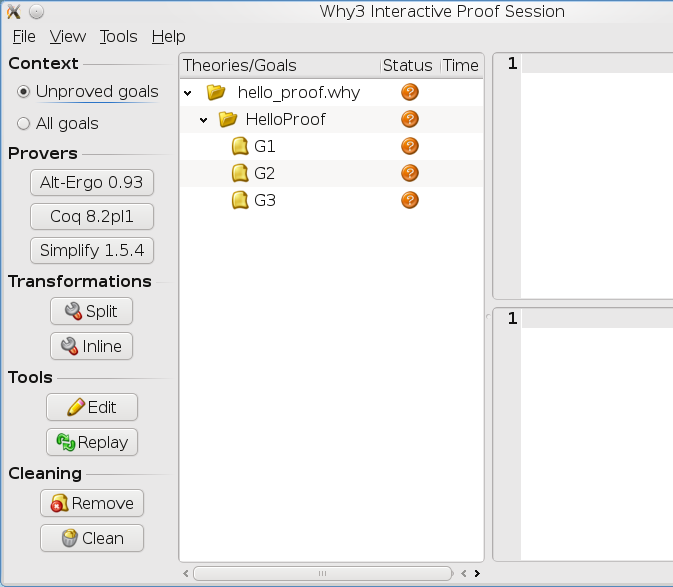
\includegraphics[width=\textwidth]{gui-0-70-1.png}
  \caption{The GUI when started the very first time}
  \label{fig:gui1}
\end{figure}

The GUI is launched on the file above as follows.
\begin{verbatim}
why3 ide hello_proof.why
\end{verbatim}
When the GUI is started for the first time, you should get a window
that looks like the screenshot of Figure~\ref{fig:gui1}.

The left column is a tool bar which provides different actions to
apply on goals. The section ``Provers'' displays the provers that were
detected as installed on your computer.%
%BEGIN LATEX
\footnote{If not done yet, you
  must perform prover autodetection using \texttt{why3 config
    -{}-detect-provers}}
%END LATEX
%HEVEA {} (If not done yet, you must perform prover autodetection using \texttt{why3 config -{}-detect-provers}.)
Three provers were detected, in this case,
these are Alt-Ergo~\cite{ergo}, Coq~\cite{CoqArt} and
Simplify~\cite{simplify05}.

The middle part is a tree view that
allows to browse inside the theories.
% Initially, the item of this tree
% are closed. We can expand this view using the menu \textsf{View/Expand
%   all} or its shortcut \textsf{Ctrl-E}. This will result is something
% like the screenshot of Figure~\ref{fig:gui2}.
In this tree view, we have a structured view of the file: this file
contains one theory, itself containing three goals.


\begin{figure}[tbp]
%HEVEA\centering
 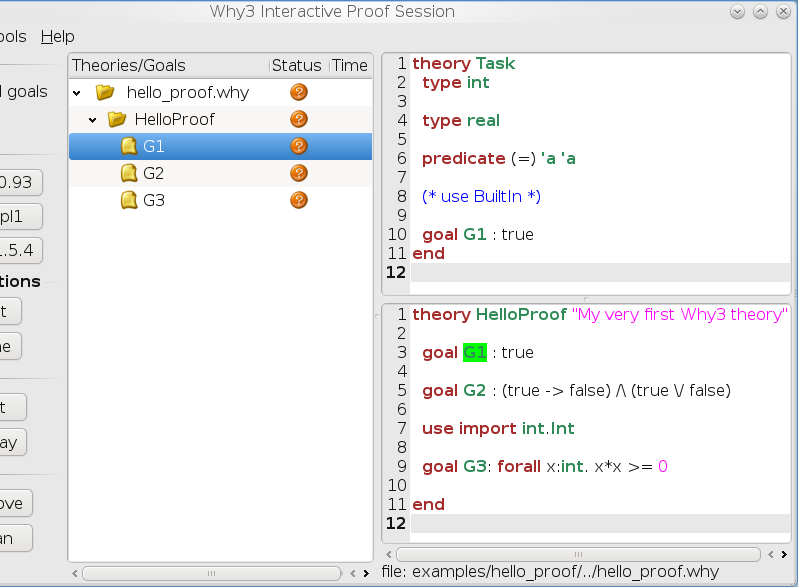
\includegraphics[width=\textwidth]{gui-0-70-2.png}
  \caption{The GUI with goal G1 selected}
  \label{fig:gui2}
\end{figure}
In Figure~\ref{fig:gui2}, we clicked on the row corresponding to
goal $G_1$. The \emph{task} associated with this goal is then
displayed on the top right, and the corresponding part of the input
file is shown on the bottom right part.


\subsection{Calling provers on goals}

You are now ready to call these provers on the goals. Whenever you
click on a prover button, this prover is called on the goal selected
in the tree view. You can select several goals at a time, either
by using multi-selection (typically by clicking while pressing the
\textsf{Shift} or \textsf{Ctrl} key) or by selecting the parent theory
or the parent file. Let us now select the theory ``HelloProof'' and
click on the \textsf{Simplify} button. After a short time, you should
get the display of Figure~\ref{fig:gui3}.

\begin{figure}[tbp]
%HEVEA\centering
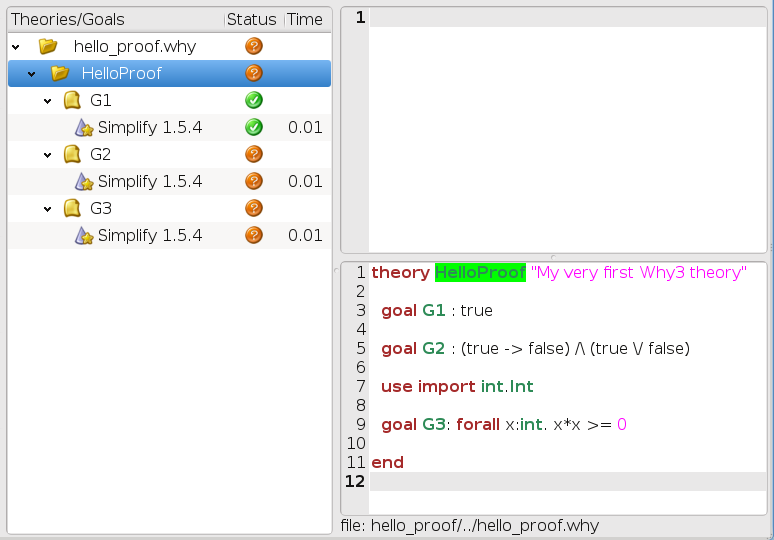
\includegraphics[width=\textwidth]{gui-0-70-3.png}
  \caption{The GUI after Simplify prover is run on each goal}
  \label{fig:gui3}
\end{figure}

Goal $G_1$ is now marked with a green ``checked'' icon in the
status column. This means that the goal is proved by the Simplify
prover. On the contrary, the two other goals are not proved, they remain
marked with an orange question mark.

You can immediately attempt to prove the remaining goals using another
prover, \eg Alt-Ergo, by clicking on the corresponding button.
Goal $G_3$ should be proved now, but not $G_2$.

\subsection{Applying transformations}

Instead of calling a prover on a goal, you can apply a transformation
to it.  Since $G_2$ is a conjunction, a possibility is to split it
into subgoals. You can do that by clicking on the \textsf{Split}
button of section ``Transformations'' of the left toolbar. Now you
have two subgoals, and you can try again a prover on them, for example
Simplify. We already have a lot of goals and proof attempts, so it is a good idea to close the sub-trees which are already proved: this can be done by the menu \textsf{View/Collapse proved goals}, or even better by its shortcut ``Ctrl-C''.
You should see now what is displayed on Figure~\ref{fig:gui4}.

\begin{figure}[tbp]
%HEVEA\centering
 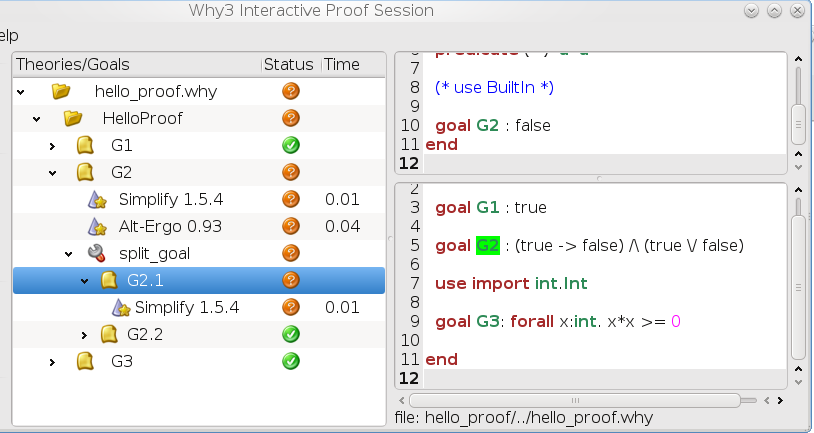
\includegraphics[width=\textwidth]{gui-0-70-4.png}
  \caption{The GUI after splitting goal $G_2$ and collapsing proved goals}
  \label{fig:gui4}
\end{figure}

The first part of goal $G_2$ is still unproved. As a last resort, we
can try to call the Coq proof assistant. The first step is to click on
the \textsf{Coq} button. A new sub-row appear for Coq, and
unsurprisingly the goal is not proved by Coq either. What can be done
now is editing the proof: select that row and then click on the
\textsf{Edit} button in section ``Tools'' of the toolbar. This should
launch the Coq proof editor, which is \texttt{coqide} by default (see
Section~\ref{sec:ideref} for details on how to configure this). You get
now a regular Coq file to fill in, as shown on Figure~\ref{fig:coqide}.
Please be mindful of the comments of this file. They indicate where \why
expects you to fill the blanks. Note that the comments themselves should
not be removed, as they are needed to properly regenerate the file when the
goal is changed. See Section~\ref{sec:coq} for more details.

\begin{figure}[tbp]
%HEVEA\centering
  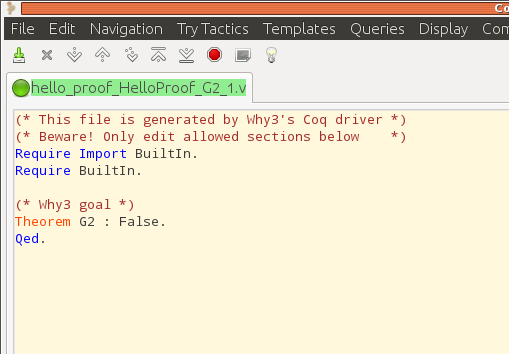
\includegraphics[width=\textwidth]{coqide-0-81.png}
  \caption{CoqIDE on subgoal 1 of $G_2$}
  \label{fig:coqide}
\end{figure}

Of course, in that particular case, the goal cannot be proved since it
is not valid. The only thing to do is to fix the input file, as
explained below.

\subsection{Modifying the input}

Currently, the GUI does not allow to modify the input file. You must
edit the file external by some editor of your choice. Let us assume we
change the goal $G_2$ by replacing the first occurrence of true by
false, \eg
\begin{whycode}
  goal G2 : (false -> false) /\ (true \/ false)
\end{whycode}
We can reload the modified file in the IDE using menu \textsf{File/Reload}, or the shortcut ``Ctrl-R''. We get the tree view shown on Figure~\ref{fig:gui5}.

\begin{figure}[tbp]
%HEVEA\centering
  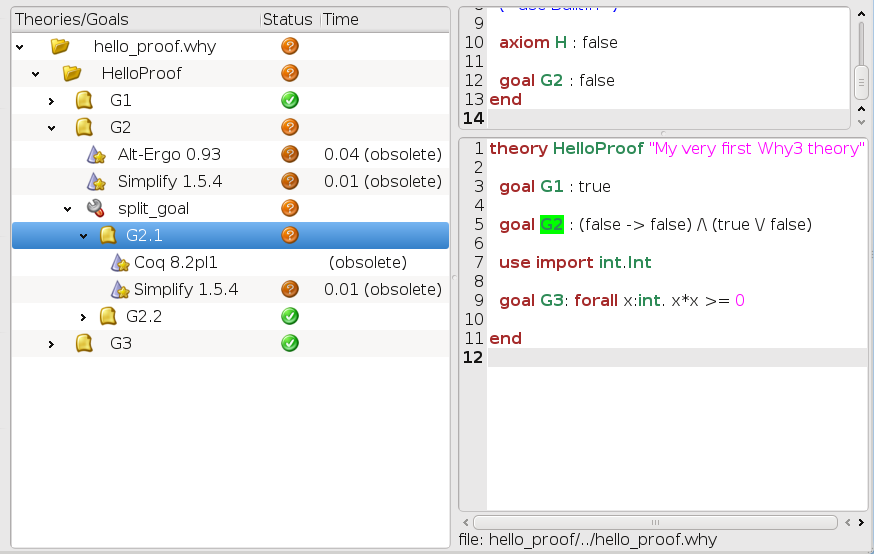
\includegraphics[width=\textwidth]{gui-0-70-5.png}
  \caption{File reloaded after modifying goal $G_2$}
  \label{fig:gui5}
\end{figure}

The important feature to notice first is that all the previous proof
attempts and transformations were saved in a database --- an XML file
created when the \why file was opened in the GUI for the first
time. Then, for all the goals that remain unchanged, the previous
proofs are shown again. For the parts that changed, the previous
proofs attempts are shown but marked with ``(obsolete)''\index{obsolete!proof attempt}
so that you
know the results are not accurate. You can now retry to prove all what
remains unproved using any of the provers.

\subsection{Replaying obsolete proofs}

Instead of pushing a prover's button to rerun its proofs, you can
\emph{replay} the existing but obsolete
proof attempts, by clicking on
the \textsf{Replay} button. By default, \textsf{Replay} only replays
proofs that were successful before. If you want to replay all of them,
you must select the context \textsf{all goals} at the top of the left
tool bar.

Notice that replaying can be done in batch mode, using the
\texttt{replay} command (see Section~\ref{sec:why3replayer}) For
example, running the replayer on the \texttt{hello\_proof} example is
as follows (assuming $G_2$ still is
\lstinline|(true -> false) /\ (true \/ false)|).
\begin{verbatim}
$ why3 replay hello_proof
Info: found directory 'hello_proof' for the project
Opening session...[Xml warning] prolog ignored
[Reload] file '../hello_proof.why'
[Reload] theory 'HelloProof'
[Reload] transformation split_goal for goal G2
 done
Progress: 9/9
 2/3
   +--file ../hello_proof.why: 2/3
      +--theory HelloProof: 2/3
         +--goal G2 not proved
Everything OK.
\end{verbatim}
The last line tells us that no differences were detected between the
current run and the run stored in the XML file. The tree above
reminds us that $G_2$ is not proved.

\subsection{Cleaning}

You may want to clean some the proof attempts, \eg removing the
unsuccessful ones when a project is finally fully proved.

A proof or a transformation can be removed by selecting it and
clicking on button \textsf{Remove}. You must confirm the
removal. Beware that there is no way to undo such a removal.

The \textsf{Clean} button performs an automatic removal of all proofs
attempts that are unsuccessful, while there exists a successful proof
attempt for the same goal.

\section{Getting Started with the \why Command}
\label{sec:batch}

The \texttt{prove} command makes it possible to check the validity of goals with external
provers, in batch mode. This section presents the basic use of this
tool. Refer to Section~\ref{sec:why3ref} for a more complete
description of this tool and all its command-line options.

The very first time you want to use \why, you should proceed with
autodetection of external provers. We have already seen how to do
it in the \why GUI. On the command line, this is done as follows
(here ``\texttt{>}'' is the prompt):
\begin{verbatim}
> why3 config --detect
\end{verbatim}
This prints some information messages on what detections are attempted. To know which
provers have been successfully detected, you can do as follows.
\begin{verbatim}
> why3 --list-provers
Known provers:
  alt-ergo (Alt-Ergo)
  coq (Coq)
  simplify (Simplify)
\end{verbatim}
The first word of each line is a unique identifier for the associated prover. We thus
have now the three provers Alt-Ergo~\cite{ergo}, Coq~\cite{CoqArt} and
Simplify~\cite{simplify05}.

Let us assume that we want to run Simplify on the HelloProof
example. The command to type and its output are as follows, where the
\verb|-P| option is followed by the unique prover identifier (as shown
by \verb|--list-provers| option).
\begin{verbatim}
> why3 prove -P simplify hello_proof.why
hello_proof.why HelloProof G1 : Valid (0.10s)
hello_proof.why HelloProof G2 : Unknown: Unknown (0.01s)
hello_proof.why HelloProof G3 : Unknown: Unknown (0.00s)
\end{verbatim}
Unlike the \why GUI, the command-line tool does not save the proof attempts
or applied transformations in a database.

We can also specify which goal or goals to prove. This is done by giving
first a theory identifier, then goal identifier(s). Here is the way to
call Alt-Ergo on goals $G_2$ and $G_3$.
\begin{verbatim}
> why3 prove -P alt-ergo hello_proof.why -T HelloProof -G G2 -G G3
hello_proof.why HelloProof G2 : Unknown: Unknown (0.01s)
hello_proof.why HelloProof G3 : Valid (0.01s)
\end{verbatim}

Finally, a transformation to apply to goals before proving them can be
specified. To know the unique identifier associated to
a transformation, do as follows.
\begin{verbatim}
> why3 --list-transforms
Known non-splitting transformations:
  [...]

Known splitting transformations:
  [...]
  split_goal
  split_intro
\end{verbatim}
Here is how you can split the goal $G_2$ before calling
Simplify on the resulting subgoals.
\begin{verbatim}
> why3 prove -P simplify hello_proof.why -a split_goal -T HelloProof -G G2
hello_proof.why HelloProof G2 : Unknown: Unknown (0.00s)
hello_proof.why HelloProof G2 : Valid (0.00s)
\end{verbatim}
Section~\ref{sec:transformations} gives the description of the various
transformations available.

%%% Local Variables:
%%% mode: latex
%%% TeX-PDF-mode: t
%%% TeX-master: "manual"
%%% End:


\chapter{Syntax}

This chapter describes the input syntax, and informally gives its semantics,
illustrated by examples.

\section{Terms and Formulas}

\section{Declarations, Theories}


%%% Local Variables:
%%% mode: latex
%%% TeX-PDF-mode: t
%%% TeX-master: "manual"
%%% End:


% \chapter{Tools}
\label{chap:tools}

\section{\why\ command line tool}

\section{IDE}

The graphical interface allows to browse into a file or a set of
files, and check the validity of goals with external provers, in a
friendly way. This section presents the basic use of this GUI. Please refer to Section~\ref{sec:ideref} for a more complete description.

\section{Other tools}

\begin{itemize}
\item why-config
\item why-bench
\end{itemize}



%%% Local Variables:
%%% mode: latex
%%% TeX-PDF-mode: t
%%% TeX-master: "manual"
%%% End:


\chapter{The WhyML Programming Language}
\label{chap:whyml}

This chapter describes the \whyml programming language.
A \whyml input text contains a list of theories (see
chapter~\ref{chap:syntax}) and/or modules.
Modules extend theories with \emph{programs}.
Programs can use all types, symbols, and constructs from the logic.
They also provide extra features:
\begin{itemize}
\item
  In a record type declaration, some fields can be declared
  \texttt{mutable}.
\item
  There are programming constructs with no counterpart in the logic:
  \begin{itemize}
  \item mutable field assignment;
  \item sequence;
  \item loops;
  \item exceptions;
  \item local and anonymous functions;
  \item annotations: pre- and postconditions, assertions, loop invariants.
  \end{itemize}
\item
  A program function can be non-terminating or can be proved
  to be terminating using a variant (a term together with a well-founded
  order relation).
\item
  An abstract program type $t$ can be introduced with a logical
  \emph{model} $\tau$: inside programs, $t$ is abstract, and inside
  annotations, $t$ is an alias for $\tau$.
\end{itemize}
%
Programs are contained in files with suffix \verb|.mlw|.
They are handled by \texttt{why3}. For instance
\begin{verbatim}
  % why3 myfile.mlw
\end{verbatim}
will display the verification conditions extracted from modules in
file \texttt{myfile.mlw}, as a set of corresponding theories, and
\begin{verbatim}
  % why3 -P alt-ergo myfile.mlw
\end{verbatim}
will run the SMT solver Alt-Ergo on these verification conditions.
Program files are also handled by the GUI tool \texttt{why3ide}.
See Chapter~\ref{chap:manpages} for more details regarding command lines.

\medskip
As an introduction to \whyml, we use the five problems from the VSTTE
2010 verification competition~\cite{vstte10comp}.
The source code for all these examples is contained in \why's
distribution, in sub-directory \texttt{examples/programs/}.

\section{Problem 1: Sum and Maximum}

The first problem is stated as follows:
\begin{quote}
  Given an $N$-element array of natural numbers,
  write a program to compute the sum and the maximum of the
  elements in the array.
\end{quote}
We  assume $N \ge 0$ and $a[i] \ge 0$ for $0 \le i < N$, as precondition,
and we have to prove the following postcondition:
\begin{displaymath}
  sum \le N \times max.
\end{displaymath}
In a file \verb|max_sum.mlw|, we start a new module:
\begin{verbatim}
  module MaxAndSum
\end{verbatim}
We are obviously needing arithmetic, so we import the corresponding
theory, exactly as we would do within a theory definition:
\begin{verbatim}
    use import int.Int
\end{verbatim}
We are also going to use references and arrays from \whyml's standard
library, so we import the corresponding modules, with a similar
declaration:
\begin{verbatim}
    use import module ref.Ref
    use import module array.Array
\end{verbatim}
The additional keyword \texttt{module} means that we are looking for
\texttt{.mlw} files from the standard library (namely \texttt{ref.mlw}
and \texttt{array.mlw} here), instead of \texttt{.why} files.
Modules \texttt{Ref} and \texttt{Array} respectively provide a type
\texttt{ref 'a} for references and a type \texttt{array 'a} for
arrays (see Section~\ref{sec:mllibrary}), together with useful
operations and traditional syntax.

We are now in position to define a program function
\verb|max_sum|. A function definition is introduced with the keyword
\texttt{let}. In our case, it introduces a function with two arguments,
an array \texttt{a} and its size \texttt{n}:
\begin{verbatim}
    let max_sum (a: array int) (n: int) = ...
\end{verbatim}
(There is a function \texttt{length} to get the size of an array but
we add this extra parameter \texttt{n} to stay close to the original
problem statement.) The function body is a Hoare triple, that is a
precondition, a program expression, and a postcondition.
\begin{verbatim}
    let max_sum (a: array int) (n: int) =
      { 0 <= n = length a /\ forall i:int. 0 <= i < n -> a[i] >= 0 }
       ... expression ...
      { let (sum, max) = result in sum <= n * max }
\end{verbatim}
The precondition expresses that \texttt{n} is non-negative and is
equal to the length of \texttt{a} (this will be needed for
verification conditions related to array bound checking), and that all
elements of \texttt{a} are non-negative.
The postcondition assumes that the value returned by the function,
denoted \texttt{result}, is a pair of integers, and decomposes it as
the pair \texttt{(sum, max)} to express the required property.

We are now left with the function body itself, that is a code
computing the sum and the maximum of all elements in \texttt{a}. With
no surpise, it is as simple as introducing two local references
\begin{verbatim}
    let sum = ref 0 in
    let max = ref 0 in
\end{verbatim}
scanning the array with a \texttt{for} loop, updating \texttt{max}
and \texttt{sum}
\begin{verbatim}
    for i = 0 to n - 1 do
      if !max < a[i] then max := a[i];
      sum := !sum + a[i]
    done;
\end{verbatim}
and finally returning the pair of the values contained in \texttt{sum}
and \texttt{max}:
\begin{verbatim}
    (!sum, !max)
\end{verbatim}
This completes the code for function \texttt{max\_sum}.
As such, it cannot be proved correct, since the loop is still lacking
a loop invariant. In this case, the loop invariant is as simple as
\verb|!sum <= i * !max|, since the postcondition only requires to prove
\verb|sum <= n * max|. The loop invariant is introduced with the
keyword \texttt{invariant}, immediately after the keyword \texttt{do}.
\begin{verbatim}
      for i = 0 to n - 1 do
        invariant { !sum <= i * !max }
        ...
      done
\end{verbatim}
There is no need to introduce a variant, as the termination of a
\texttt{for} loop is automatically guaranteed.
This completes module \texttt{MaxAndSum}.
Figure~\ref{fig:MaxAndSum} shows the whole code.
\begin{figure}
  \centering
\begin{verbatim}
module MaxAndSum

  use import int.Int
  use import module ref.Ref
  use import module array.Array

  let max_sum (a: array int) (n: int) =
    { 0 <= n = length a /\ forall i:int. 0 <= i < n -> a[i] >= 0 }
    let sum = ref 0 in
    let max = ref 0 in
    for i = 0 to n - 1 do
      invariant { !sum <= i * !max }
      if !max < a[i] then max := a[i];
      sum := !sum + a[i]
    done;
    (!sum, !max)
    { let (sum, max) = result in sum <= n * max }

end
\end{verbatim}
\vspace*{-2em}\hrulefill
  \caption{Solution for VSTTE'10 competition problem 1.}
  \label{fig:MaxAndSum}
\end{figure}
We can now proceed to its verification.
Running \texttt{why3}, or better \texttt{why3ide}, on file
\verb|max_sum.mlw| will show a single verification condition with name
\verb|WP_parameter_max_sum|.
Discharging this verification condition with an automated theorem
prover will not succeed, most likely, as it involves non-linear
arithmetic. Repeated applications of goal splitting and calls to
SMT solvers (within \texttt{why3ide}) will typically leave a single,
unsolved goal, which reduces to proving the following sequent:
\begin{displaymath}
  s \le i \times max, ~ max < a[i] \vdash s + a[i] \le (i+1) \times a[i].
\end{displaymath}
This is easily discharged using an interactive proof assistant such as
Coq, and thus completes the verification.

\section{Problem 2: Inverting an Injection}

The second problem is stated as follows:
\begin{quote}
  Invert an injective array $A$ on $N$ elements in the
  subrange from $0$ to $N - 1$, i.e., the output array $B$ must be
  such that $B[A[i]] = i$ for $0 \le i < N$.
\end{quote}
We may assume that $A$ is surjective and we have to prove
that the resulting array is also injective.
The code is immediate, since it is as simple as
\begin{verbatim}
    for i = 0 to n - 1 do b[a[i]] <- i done
\end{verbatim}
so it is more a matter of specification and of getting the proof done
with as much automation as possible. In a new file, we start a new
module and we import arithmetic and arrays:
\begin{verbatim}
  module InvertingAnInjection
    use import int.Int
    use import module array.Array
\end{verbatim}
It is convenient to introduce predicate definitions for the properties
of being injective and surjective. These are purely logical
declarations:
\begin{verbatim}
    predicate injective (a: array int) (n: int) =
      forall i j: int. 0 <= i < n -> 0 <= j < n -> i <> j -> a[i] <> a[j]

    predicate surjective (a: array int) (n: int) =
      forall i: int. 0 <= i < n -> exists j: int. (0 <= j < n /\ a[j] = i)
\end{verbatim}
It is also convenient to introduce the predicate ``being in the
subrange from 0 to $n-1$'':
\begin{verbatim}
    predicate range (a: array int) (n: int) =
      forall i: int. 0 <= i < n -> 0 <= a[i] < n
\end{verbatim}
Using these predicates, we can formulate the assumption that any
injective array of size $n$ within the range $0..n-1$ is also surjective:
\begin{verbatim}
    lemma injective_surjective:
      forall a: array int, n: int.
      injective a n -> range a n -> surjective a n
\end{verbatim}
We declare it as a lemma rather than as an axiom, since it is actually
provable. It requires induction and can be proved using the Coq proof
assistant for instance.
Finally we can give the code a specification, with a loop invariant
which simply expresses the values assigned to array \texttt{b} so far:
\begin{verbatim}
    let inverting (a: array int) (b: array int) (n: int) =
      { 0 <= n = length a = length b /\ injective a n /\ range a n }
      for i = 0 to n - 1 do
        invariant { forall j: int. 0 <= j < i -> b[a[j]] = j }
        b[a[i]] <- i
      done
      { injective b n }
\end{verbatim}
Here we chose to have array \texttt{b} as argument; returning a
freshly allocated array would be equally simple.
The whole module is given Figure~\ref{fig:Inverting}.
The verification conditions for function \texttt{inverting} are easily
discharged automatically, thanks to the lemma.
\begin{figure}
  \centering
\begin{verbatim}
module InvertingAnInjection

  use import int.Int
  use import module array.Array

  predicate injective (a: array int) (n: int) =
    forall i j: int. 0 <= i < n -> 0 <= j < n -> i <> j -> a[i] <> a[j]

  predicate surjective (a: array int) (n: int) =
    forall i: int. 0 <= i < n -> exists j: int. (0 <= j < n /\ a[j] = i)

  predicate range (a: array int) (n: int) =
    forall i: int. 0 <= i < n -> 0 <= a[i] < n

  lemma injective_surjective:
    forall a: array int, n: int.
    injective a n -> range a n -> surjective a n

  let inverting (a: array int) (b: array int) (n: int) =
    { 0 <= n = length a = length b /\ injective a n /\ range a n }
    for i = 0 to n - 1 do
      invariant { forall j: int. 0 <= j < i -> b[a[j]] = j }
      b[a[i]] <- i
    done
    { injective b n }

end
\end{verbatim}
\vspace*{-2em}\hrulefill
  \caption{Solution for VSTTE'10 competition problem 2.}
  \label{fig:Inverting}
\end{figure}

\section{Problem 3: Searching a Linked List}

The third problem is stated as follows:
\begin{quote}
  Given a linked list representation of a list of integers,
  find the index of the first element that is equal to 0.
\end{quote}
More precisely, the specification says
\begin{quote}
  You have to show that the program returns an index $i$ equal to the
  length of the list if there is no such element. Otherwise, the $i$-th
  element of the list must be equal to 0, and all the preceding
  elements must be non-zero.
\end{quote}
Since the list is not mutated, we can use the algebraic data type of
polymorphic lists from \why's standard library, defined in theory
\texttt{list.List}. It comes with other handy theories:
\texttt{list.Length}, which provides a function \texttt{length}, and
\texttt{list.Nth}, which provides a function \texttt{nth}
for the $n$-th element of a list. The latter returns an option type,
depending on whether the index is meaningful or not.
\begin{verbatim}
  module SearchingALinkedList
    use import int.Int
    use export list.List
    use export list.Length
    use export list.Nth
\end{verbatim}
It is helpful to introduce two predicates: a first one
for a successful search,
\begin{verbatim}
    predicate zero_at (l: list int) (i: int) =
      nth i l = Some 0 /\ forall j:int. 0 <= j < i -> nth j l <> Some 0
\end{verbatim}
and another for a non-successful search,
\begin{verbatim}
    predicate no_zero (l: list int) =
      forall j:int. 0 <= j < length l -> nth j l <> Some 0
\end{verbatim}
We are now in position to give the code for the search function.
We write it as a recursive function \texttt{search} that scans a list
for the first zero value:
\begin{verbatim}
    let rec search (i: int) (l: list int) = match l with
      | Nil      -> i
      | Cons x r -> if x = 0 then i else search (i+1) r
      end
\end{verbatim}
Passing an index \texttt{i} as first argument allows to perform a tail
call. A simpler code (yet less efficient) would return 0 in the first
branch and \texttt{1 + search ...} in the second one, avoiding the
extra argument \texttt{i}.

We first prove the termination of this recursive function. It amounts
to give it a \emph{variant}, that is an term integer term which stays
non-negative and strictly decreases at each recursive call. Here it is
as simple as the length of \texttt{l}:
\begin{verbatim}
    let rec search (i: int) (l: list int) variant { length l } = ...
\end{verbatim}
(It is worth pointing out that variants are not limited to natural
numbers. Any other type equipped with a well-founded order relation
can be used instead.)
There is no precondition for function \texttt{search}.
The postcondition expresses that either a zero value is found, and
consequently the value returned is bounded accordingly,
\begin{verbatim}
  i <= result < i + length l /\ zero_at l (result - i)
\end{verbatim}
or no zero value was found, and thus the returned value is exactly
\texttt{i} plus the length of \texttt{l}:
\begin{verbatim}
  result = i + length l /\ no_zero l
\end{verbatim}
Solving the problem is simply a matter of calling \texttt{search} with
0 as first argument.
The code is given Figure~\ref{fig:LinkedList}. The verification
conditions are all discharged automatically.
\begin{figure}
  \centering
\begin{verbatim}
module SearchingALinkedList

  use import int.Int
  use export list.List
  use export list.Length
  use export list.Nth

  predicate zero_at (l: list int) (i: int) =
    nth i l = Some 0 /\ forall j:int. 0 <= j < i -> nth j l <> Some 0

  predicate no_zero (l: list int) =
    forall j:int. 0 <= j < length l -> nth j l <> Some 0

  let rec search (i: int) (l: list int) variant { length l } =
    {}
    match l with
    | Nil -> i
    | Cons x r -> if x = 0 then i else search (i+1) r
    end
    { (i <= result < i + length l /\ zero_at l (result - i))
      \/
      (result = i + length l /\ no_zero l) }

  let search_list (l: list int) =
    { }
    search 0 l
    { (0 <= result < length l /\ zero_at l result)
      \/
      (result = length l /\ no_zero l) }

end
\end{verbatim}
\vspace*{-2em}\hrulefill
  \caption{Solution for VSTTE'10 competition problem 3.}
  \label{fig:LinkedList}
\end{figure}

Alternatively, we can implement the search with a \texttt{while} loop.
To do this, we need to import references from the standard library,
together with theory \texttt{list.HdTl} which defines function
\texttt{hd} and \texttt{tl} over lists.
\begin{verbatim}
    use import module ref.Ref
    use import list.HdTl
\end{verbatim}
Being partial functions, \texttt{hd} and \texttt{tl} return options.
For the purpose of our code, though, it is simpler to have functions
which do not return options, but have preconditions instead. Such a
function \texttt{head} is defined as follows:
\begin{verbatim}
    let head (l: list 'a) =
      { l <> Nil }
      match l with Nil -> absurd | Cons h _ -> h end
      { hd l = Some result }
\end{verbatim}
The program construct \texttt{absurd} denotes an unreachable piece of
code. It generates the verification condition \texttt{false}, which is
here provable using the precondition (the list cannot be \texttt{Nil}).
Function \texttt{tail} is defined similarly:
\begin{verbatim}
    let tail (l : list 'a) =
      { l <> Nil }
      match l with Nil -> absurd | Cons _ t -> t end
      { tl l = Some result }
\end{verbatim}
Using \texttt{head} and \texttt{tail}, it is straightforward to
implement the search as a \texttt{while} loop.
It uses a local reference \texttt{i} to store the index and another
local reference \texttt{s} to store the list being scanned.
As long as \texttt{s} is not empty and its head is not zero, it
increments \texttt{i} and advances in \texttt{s} using function \texttt{tail}.
\begin{verbatim}
    let search_loop l =
      { }
      let i = ref 0 in
      let s = ref l in
      while !s <> Nil && head !s <> 0 do
        invariant { ... }
        variant   { length !s }
        i := !i + 1;
        s := tail !s
      done;
      !i
      { ... same postcondition as search_list ... }
\end{verbatim}
The postcondition is exactly the same as for function \verb|search_list|.
The termination of the \texttt{while} loop is ensured using a variant,
exactly as for a recursive function. Such a variant must strictly decrease at
each execution of the loop body. The reader is invited to figure out
the loop invariant.

\section{Problem 4: N-Queens}

The fourth problem is probably the most challenging one.
We have to verify the implementation of a program which solves the
$N$-queens puzzle: place $N$ queens on an $N \times N$
chess board so that no queen can capture another one with a
legal move.
The program should return a placement if there is a solution and
indicates that there is no solution otherwise. A placement is a
$N$-element array which assigns the queen on row $i$ to its column.
Thus we start our module by importing arithmetic and arrays:
\begin{verbatim}
  module NQueens
    use import int.Int
    use import module array.Array
\end{verbatim}
The code is a simple backtracking algorithm, which tries to put a queen
on each row of the chess board, one by one (there is basically no
better way to solve the $N$-queens puzzle).
A building block is a function which checks whether the queen on a
given row may attack another queen on a previous row. To verify this
function, we first define a more elementary predicate, which expresses
that queens on row \texttt{pos} and \texttt{q} do no attack each other:
\begin{verbatim}
    predicate consistent_row (board: array int) (pos: int) (q: int) =
      board[q] <> board[pos] /\
      board[q] - board[pos] <> pos - q /\
      board[pos] - board[q] <> pos - q
\end{verbatim}
Then it is possible to define the consistency of row \texttt{pos}
with respect to all previous rows:
\begin{verbatim}
    predicate is_consistent (board: array int) (pos: int) =
      forall q:int. 0 <= q < pos -> consistent_row board pos q
\end{verbatim}
Implementing a function which decides this predicate is another
matter. In order for it to be efficient, we want to return
\texttt{False} as soon as a queen attacks the queen on row
\texttt{pos}. We use an exception for this purpose and it carries the
row of the attacking queen:
\begin{verbatim}
    exception Inconsistent int
\end{verbatim}
The check is implemented by a function \verb|check_is_consistent|,
which takes the board and the row \texttt{pos} as arguments, and scans
rows from 0 to \texttt{pos-1} looking for an attacking queen. As soon
as one is found, the exception is raised. It is caught immediately
outside the loop and \texttt{False} is returned. Whenever the end of
the loop is reached, \texttt{True} is returned.
\begin{verbatim}
    let check_is_consistent (board: array int) (pos: int) =
      { 0 <= pos < length board }
      try
        for q = 0 to pos - 1 do
          invariant {
            forall j:int. 0 <= j < q -> consistent_row board pos j
          }
          let bq   = board[q]   in
          let bpos = board[pos] in
          if bq        = bpos    then raise (Inconsistent q);
          if bq - bpos = pos - q then raise (Inconsistent q);
          if bpos - bq = pos - q then raise (Inconsistent q)
        done;
        True
      with Inconsistent q ->
        assert { not (consistent_row board pos q) };
        False
      end
      { result=True <-> is_consistent board pos }
\end{verbatim}
The assertion in the exception handler is a cut for SMT solvers.
This first part of the solution is given Figure~\ref{fig:NQueens1}.
\begin{figure}
  \centering
\begin{verbatim}
module NQueens
  use import int.Int
  use import module array.Array

  predicate consistent_row (board: array int) (pos: int) (q: int) =
    board[q] <> board[pos] /\
    board[q] - board[pos] <> pos - q /\
    board[pos] - board[q] <> pos - q

  predicate is_consistent (board: array int) (pos: int) =
    forall q:int. 0 <= q < pos -> consistent_row board pos q

  exception Inconsistent int

  let check_is_consistent (board: array int) (pos: int) =
    { 0 <= pos < length board }
    try
      for q = 0 to pos - 1 do
        invariant {
          forall j:int. 0 <= j < q -> consistent_row board pos j
        }
        let bq   = board[q]   in
        let bpos = board[pos] in
        if bq        = bpos    then raise (Inconsistent q);
        if bq - bpos = pos - q then raise (Inconsistent q);
        if bpos - bq = pos - q then raise (Inconsistent q)
      done;
      True
    with Inconsistent q ->
      assert { not (consistent_row board pos q) };
      False
    end
    { result=True <-> is_consistent board pos }
\end{verbatim}
\vspace*{-2em}\hrulefill
  \caption{Solution for VSTTE'10 competition problem 4 (1/2).}
  \label{fig:NQueens1}
\end{figure}

We now proceed with the verification of the backtracking algorithm.
The specification requires us to define the notion of solution, which
is straightforward using the predicate \verb|is_consistent| above.
However, since the algorithm will try to complete a given partial
solution, it is more convenient to define the notion of partial
solution, up to a given row. It is even more convenient to split it in
two predicates, one related to legal column values and another to
consistency of rows:
\begin{verbatim}
    predicate is_board (board: array int) (pos: int) =
      forall q:int. 0 <= q < pos -> 0 <= board[q] < length board

    predicate solution (board: array int) (pos: int) =
      is_board board pos /\
      forall q:int. 0 <= q < pos -> is_consistent board q
\end{verbatim}
The algorithm will not mutate the partial solution it is given and,
in case of a search failure, will claim that there is no solution
extending this prefix. For this reason, we introduce a predicate
comparing two chess boards for equality up to a given row:
\begin{verbatim}
    predicate eq_board (b1 b2: array int) (pos: int) =
      forall q:int. 0 <= q < pos -> b1[q] = b2[q]
\end{verbatim}
The search itself makes use of an exception to signal a successful search:
\begin{verbatim}
    exception Solution
\end{verbatim}
The backtracking code is a recursive function \verb|bt_queens| which
takes the chess board, its size, and the starting row for the search.
The termination is ensured by the obvious variant \texttt{n-pos}.
\begin{verbatim}
    let rec bt_queens (board: array int) (n: int) (pos: int) 
                      variant {n-pos} =
\end{verbatim}
The precondition relates \texttt{board}, \texttt{pos}, and \texttt{n}
and requires \texttt{board} to be a solution up to \texttt{pos}:
\begin{verbatim}
      { length board = n /\ 0 <= pos <= n /\ solution board pos }
      'Init:
\end{verbatim}
We place a code mark \texttt{'Init} immediately after the precondition to
be able to refer to the value of \texttt{board} in the pre-state.
Whenever we reach the end of the chess board, we have found a solution
and we signal it using exception \texttt{Solution}:
\begin{verbatim}
      if pos = n then raise Solution;
\end{verbatim}
Otherwise we scan all possible positions for the queen on row
\texttt{pos} with a \texttt{for} loop:
\begin{verbatim}
      for i = 0 to n - 1 do
\end{verbatim}
The loop invariant states that we have not modified the solution
prefix so far, and that we have not found any solution that would
extend this prefix with a queen on row \texttt{pos} at a column below
\texttt{i}:
\begin{verbatim}
        invariant {
          eq_board board (at board 'Init) pos /\
          forall b:array int. length b = n -> is_board b n ->
            eq_board board b pos -> 0 <= b[pos] < i ->
              not (solution b n) }
\end{verbatim}
Then we assign column \texttt{i} to the queen on row \texttt{pos} and
we check for a possible attack with \verb|check_is_consistent|. If
not, we call \verb|bt_queens| recursively on the next row.
\begin{verbatim}
        board[pos] <- i;
        if check_is_consistent board pos then bt_queens board n (pos + 1)
      done
\end{verbatim}
This completes the loop and function \verb|bt_queens| as well.
The postcondition is twofold: either the function exits normally and
then there is no solution extending the prefix in \texttt{board},
which has not been modified;
or the function raises \texttt{Solution} and we have a solution in
\texttt{board}.
\begin{verbatim}
      { eq_board board (old board) pos /\
        forall b:array int. length b = n -> is_board b n ->
          eq_board board b pos -> not (solution b n) }
      | Solution ->
      { solution board n }
\end{verbatim}
Solving the puzzle is a simple call to \verb|bt_queens|, starting the
search on row 0. The postcondition is also twofold, as for
\verb|bt_queens|, yet slightly simpler.
\begin{verbatim}
    let queens (board: array int) (n: int) =
      { 0 <= length board = n }
      bt_queens board n 0
      { forall b:array int. length b = n -> is_board b n ->
                              not (solution b n) }
      | Solution -> { solution board n }
\end{verbatim}
This second part of the solution is given Figure~\ref{fig:NQueens2}.
With the help of a few auxiliary lemmas --- not given here but available
from \why's sources --- the verification conditions are all discharged
automatically, including the verification of the lemmas themselves.
\begin{figure}
  \centering
\begin{verbatim}
  predicate is_board (board: array int) (pos: int) =
    forall q:int. 0 <= q < pos -> 0 <= board[q] < length board

  predicate solution (board: array int) (pos: int) =
    is_board board pos /\
    forall q:int. 0 <= q < pos -> is_consistent board q

  predicate eq_board (b1 b2: array int) (pos: int) =
    forall q:int. 0 <= q < pos -> b1[q] = b2[q]

  exception Solution

  let rec bt_queens (board: array int) (n: int) (pos: int)
                    variant { n - pos } =
    { length board = n /\ 0 <= pos <= n /\ solution board pos }
    'Init:
    if pos = n then raise Solution;
    for i = 0 to n - 1 do
      invariant {
        eq_board board (at board 'Init) pos /\
        forall b:array int. length b = n -> is_board b n ->
          eq_board board b pos -> 0 <= b[pos] < i -> not (solution b n) }
      board[pos] <- i;
      if check_is_consistent board pos then bt_queens board n (pos + 1)
    done
    { (* no solution *)
      eq_board board (old board) pos /\
      forall b:array int. length b = n -> is_board b n ->
        eq_board board b pos -> not (solution b n) }
    | Solution ->
    { (* a solution *)
      solution board n }

  let queens (board: array int) (n: int) =
    { 0 <= length board = n }
    bt_queens board n 0
    { forall b:array int. length b = n -> is_board b n ->
                            not (solution b n) }
    | Solution -> { solution board n }
end
\end{verbatim}
\vspace*{-2em}\hrulefill
  \caption{Solution for VSTTE'10 competition problem 4 (2/2).}
  \label{fig:NQueens2}
\end{figure}


\section{Problem 5: Amortized Queue}

The last problem consists in verifying the implementation of a
well-known purely applicative data structure for queues.
A queue is composed of two lists, \textit{front} and \textit{rear}.
We push elements at the head of list \textit{rear} and pop them off
the head of list \textit{front}. We maintain that the length of
\textit{front} is always greater or equal to the length of \textit{rear}.
(See for instance Okasaki's \emph{Purely Functional Data
  Structures}~\cite{okasaki98} for more details.)

We have to implement operations \texttt{empty}, \texttt{head},
\texttt{tail}, and \texttt{enqueue} over this data type,
to show that the invariant over lengths is maintained, and finally
\begin{quote}
  to show that a client invoking these operations
  observes an abstract queue given by a sequence.
\end{quote}
In a new module, we import arithmetic and theory
\texttt{list.ListRich}, a combo theory which imports all list
operations we will require: length, reversal, and concatenation.
\begin{verbatim}
  module AmortizedQueue
    use import int.Int
    use export list.ListRich
\end{verbatim}
The queue data type is naturally introduced as a polymorphic record type.
The two list lengths are explicitly stored, for better efficiency.
\begin{verbatim}
    type queue 'a = {| front: list 'a; lenf: int;
                       rear : list 'a; lenr: int; |}
\end{verbatim}
We start with the definition of the data type invariant, as a
predicate \texttt{inv}. It makes use of the ability to chain
several equalities and inequalities.
\begin{verbatim}
    predicate inv (q: queue 'a) =
      length q.front = q.lenf >= length q.rear = q.lenr
\end{verbatim}
For the purpose of the specification, it is convenient to introduce a function
\texttt{sequence} which builds the sequence of elements of a queue, that
is the front list concatenated to reversed rear list.
\begin{verbatim}
    function sequence (q: queue 'a) : list 'a =
      q.front ++ reverse q.rear
\end{verbatim}
It is worth pointing out that this function will only be used in
specifications.
We start with the easiest operation: building the empty queue.
\begin{verbatim}
  let empty () =
    {}
    {| front = Nil; lenf = 0; rear = Nil; lenr = 0 |} : queue 'a
    { inv result /\ sequence result = Nil }
\end{verbatim}
The postcondition is twofold: the returned queue satisfies its
invariant and represents the empty sequence.
Note the cast to type \texttt{queue 'a}. It is required, for the
type checker not to complain about an undefined type variable.

The next operation is \texttt{head}, which returns the first element from
a given queue \texttt{q}. It naturally requires the queue to be non
empty, which is conveniently expressed as \texttt{sequence q} not
being \texttt{Nil}.
\begin{verbatim}
  let head (q: queue 'a) =
    { inv q /\ sequence q <> Nil }
    match q.front with
      | Nil      -> absurd
      | Cons x _ -> x
    end
    { hd (sequence q) = Some result }
\end{verbatim}
Note the presence of the invariant in the precondition, which is
required to prove the absurdity of the first branch (if
\texttt{q.front} is \texttt{Nil}, then so should be \texttt{sequence q}).

The next operation is \texttt{tail}, which removes the first element
from a given queue. This is more subtle than \texttt{head}, since we
may have to re-structure the queue to maintain the invariant.
Since we will have to perform a similar operation when implementation
operation \texttt{enqueue}, it is a good idea to introduce a smart
constructor \texttt{create} which builds a queue from two lists, while
ensuring the invariant. The list lengths are also passed as arguments,
to avoid unnecessary computations.
\begin{verbatim}
    let create (f: list 'a) (lf: int) (r: list 'a) (lr: int) =
      { lf = length f /\ lr = length r }
      if lf >= lr then
        {| front = f; lenf = lf; rear = r; lenr = lr |}
      else
        let f = f ++ reverse r in
        {| front = f; lenf = lf + lr; rear = Nil; lenr = 0 |}
      { inv result /\ sequence result = f ++ reverse r }
\end{verbatim}
If the invariant already holds, it is simply a matter of building the
record. Otherwise, we empty the rear list and build a new front list
as the concatenation of list \texttt{f} and the reversal of list \texttt{r}.
The principle of this implementation is that the cost of this reversal
will be amortized over all queue operations. Implementing function
\texttt{tail} is now straightforward and follows the structure of
function \texttt{head}.
\begin{verbatim}
    let tail (q: queue 'a) =
      { inv q /\ sequence q <> Nil }
      match q.front with
        | Nil      -> absurd
        | Cons _ r -> create r (q.lenf - 1) q.rear q.lenr
      end
      { inv result /\ tl (sequence q) = Some (sequence result) }
\end{verbatim}
The last operation is \texttt{enqueue}, which pushes a new element in
a given queue. Reusing the smart constructor \texttt{create} makes it
a one line code.
\begin{verbatim}
    let enqueue (x: 'a) (q: queue 'a) =
      { inv q }
      create q.front q.lenf (Cons x q.rear) (q.lenr + 1)
      { inv result /\ sequence result = sequence q ++ Cons x Nil }
\end{verbatim}
The code is given Figure~\ref{fig:AQueue}. The verification conditions
are all discharged automatically.
\begin{figure}
  \centering
\begin{verbatim}
module AmortizedQueue
  use import int.Int
  use export list.ListRich

  type queue 'a = {| front: list 'a; lenf: int;
                     rear : list 'a; lenr: int; |}

  predicate inv (q: queue 'a) =
    length q.front = q.lenf >= length q.rear = q.lenr

  function sequence (q: queue 'a) : list 'a = q.front ++ reverse q.rear

  let empty () =
    {}
    {| front = Nil; lenf = 0; rear = Nil; lenr = 0 |} : queue 'a
    { inv result /\ sequence result = Nil }

  let head (q: queue 'a) =
    { inv q /\ sequence q <> Nil }
    match q.front with
      | Nil      -> absurd
      | Cons x _ -> x
    end
    { hd (sequence q) = Some result }

  let create (f: list 'a) (lf: int) (r: list 'a) (lr: int) =
    { lf = length f /\ lr = length r }
    if lf >= lr then
      {| front = f; lenf = lf; rear = r; lenr = lr |}
    else
      let f = f ++ reverse r in
      {| front = f; lenf = lf + lr; rear = Nil; lenr = 0 |}
    { inv result /\ sequence result = f ++ reverse r }

  let tail (q: queue 'a) =
    { inv q /\ sequence q <> Nil }
    match q.front with
      | Nil      -> absurd
      | Cons _ r -> create r (q.lenf - 1) q.rear q.lenr
    end
    { inv result /\ tl (sequence q) = Some (sequence result) }

  let enqueue (x: 'a) (q: queue 'a) =
    { inv q }
    create q.front q.lenf (Cons x q.rear) (q.lenr + 1)
    { inv result /\ sequence result = sequence q ++ Cons x Nil }
end
\end{verbatim}
\vspace*{-2em}\hrulefill
  \caption{Solution for VSTTE'10 competition problem 5.}
  \label{fig:AQueue}
\end{figure}

% other examples: same fringe ?

%%% Local Variables:
%%% compile-command: "make -C .. doc"
%%% mode: latex
%%% TeX-PDF-mode: t
%%% TeX-master: "manual"
%%% End:

% LocalWords:  surjective


\chapter{The \why API}
\label{chap:api}\index{API}
%HEVEA\cutname{api.html}

This chapter is a tutorial for the users who want to link their own
OCaml code with the \why library. We progressively introduce the way
one can use the library to build terms, formulas, theories, proof
tasks, call external provers on tasks, and apply transformations on
tasks. The complete documentation for API calls is given\begin{latexonly}
at URL~\urlapi{}.\end{latexonly}
%HEVEA at this \ahref{\urlapi}{URL}.

We assume the reader has a fair knowledge of the OCaml
language. Notice that the \why library must be installed, see
Section~\ref{sec:installlib}. The OCaml code given below is available in
the source distribution in directory \verb|examples/use_api/| together
with a few other examples.

\lstset{language={[Objective]Caml}}

\section{Building Propositional Formulas}
\label{sec:prop_form}

The first step is to know how to build propositional formulas. The
module \texttt{Term} gives a few functions for building these. Here is
a piece of OCaml code for building the formula $\mathit{true} \lor
\mathit{false}$.
\lstinputlisting{generated/logic__opening.ml}
The library uses the common type \texttt{term} both for terms
(\ie expressions that produce a value of some particular type)
and formulas (\ie boolean-valued expressions).
% To distinguish terms from formulas, one can look at the
% \texttt{t_ty} field of the \texttt{term} record: in formulas,
% this field has the value \texttt{None}, and in terms,
% \texttt{Some t}, where \texttt{t} is of type \texttt{Ty.ty}.

Such a formula can be printed using the module \texttt{Pretty}
providing pretty-printers.
\lstinputlisting{generated/logic__printformula.ml}

Assuming the lines above are written in a file \texttt{f.ml}, it can
be compiled using
\begin{verbatim}
ocamlfind ocamlc -package why3 -linkpkg f.ml -o f
\end{verbatim}
Running the generated executable \texttt{f} results in the following output.
\begin{verbatim}
formula 1 is: true \/ false
\end{verbatim}

Let us now build a formula with propositional variables: $A \land B
\rightarrow A$. Propositional variables must be declared first before
using them in formulas. This is done as follows.
\lstinputlisting{generated/logic__declarepropvars.ml}
The type \texttt{lsymbol} is the type of function and predicate symbols (which
we call logic symbols for brevity). Then the atoms $A$ and $B$ must be built
by the general function for applying a predicate symbol to a list of terms.
Here we just need the empty list of arguments.
\lstinputlisting{generated/logic__declarepropatoms.ml}

As expected, the output is as follows.
\begin{verbatim}
formula 2 is: A /\ B -> A
\end{verbatim}
Notice that the concrete syntax of \why forbids function and predicate
names to start with a capital letter (except for the algebraic type
constructors which must start with one). This constraint is not enforced
when building those directly using library calls.

\section{Building Tasks}

Let us see how we can call a prover to prove a formula. As said in
previous chapters, a prover must be given a task, so we need to build
tasks from our formulas. Task can be build incrementally from an empty
task by adding declaration to it, using the functions
\texttt{add\_*\_decl} of module \texttt{Task}. For the formula $\mathit{true} \lor
\mathit{false}$ above, this is done as follows.
\lstinputlisting{generated/logic__buildtask.ml}
To make the formula a goal, we must give a name to it, here ``goal1''. A
goal name has type \texttt{prsymbol}, for identifiers denoting
propositions in a theory or a task. Notice again that the concrete
syntax of \why requires these symbols to be capitalized, but it is not
mandatory when using the library. The second argument of
\texttt{add\_prop\_decl} is the kind of the proposition:
\texttt{Paxiom}, \texttt{Plemma} or \texttt{Pgoal}.
Notice that lemmas are not allowed in tasks
and can only be used in theories.

Once a task is built, it can be printed.
\lstinputlisting{generated/logic__printtask.ml}

The task for our second formula is a bit more complex to build, because
the variables A and B must be added as abstract (\ie not defined)
propositional symbols in the task.
\lstinputlisting{generated/logic__buildtask2.ml}

Execution of our OCaml program now outputs:
\begin{verbatim}
task 1 is:
theory Task
  goal Goal1 : true \/ false
end

task 2 is:
theory Task
  predicate A

  predicate B

  goal Goal2 : A /\ B -> A
end
\end{verbatim}

\section{Calling External Provers}
\label{sec:api:callingprovers}

To call an external prover, we need to access the \why configuration
file \texttt{why3.conf}, as it was built using the \texttt{why3config}
command line tool or the \textsf{Detect Provers} menu of the graphical
IDE. The following API calls allow to access the content of this
configuration file.
\lstinputlisting{generated/logic__getconf.ml}
The type \texttt{'a Whyconf.Mprover.t} is a map indexed by provers. A
prover is a record with a name, a version, and an alternative description
(to differentiate between various configurations of a given prover). Its
definition is in the module \texttt{Whyconf}:
\lstinputlisting{generated/whyconf__provertype.ml}
The map \texttt{provers} provides the set of existing provers.
In the following, we directly
attempt to access a prover named ``Alt-Ergo'', any version.
\lstinputlisting{generated/logic__getanyaltergo.ml}
We could also get a specific version with :
\lstinputlisting{generated/logic__getaltergo200.ml}

The next step is to obtain the driver associated to this prover. A
driver typically depends on the standard theories so these should be
loaded first.
\lstinputlisting{generated/logic__getdriver.ml}

We are now ready to call the prover on the tasks. This is done by a
function call that launches the external executable and waits for its
termination. Here is a simple way to proceed:
\lstinputlisting{generated/logic__callprover.ml}
This way to call a prover is in general too naive, since it may never
return if the prover runs without time limit. The function
\texttt{prove\_task} has an optional parameter \texttt{limit}, a record defined
in module \texttt{Call\_provers}:
\lstinputlisting{generated/call_provers__resourcelimit.ml}
where the field \texttt{limit\_time} is the maximum allowed running time in seconds,
and \texttt{limit\_mem} is the maximum allowed memory in megabytes.  The type
\texttt{prover\_result} is a record defined in module \texttt{Call\_provers}:
\lstinputlisting{generated/call_provers__proverresult.ml}
with in particular the fields:
\begin{itemize}
\item \texttt{pr\_answer}: the prover answer, explained below;
\item \texttt{pr\_time} : the time taken by the prover, in seconds.
\end{itemize}
A \texttt{pr\_answer} is the sum type defined in module \texttt{Call\_provers}:
\lstinputlisting{generated/call_provers__proveranswer.ml}
corresponding to these kinds of answers:
\begin{itemize}
\item \texttt{Valid}: the task is valid according to the prover.
\item \texttt{Invalid}: the task is invalid.
\item \texttt{Timeout}: the prover exceeds the time limit.
\item \texttt{OutOfMemory}: the prover exceeds the memory limit.
\item \texttt{Unknown} $msg$: the prover can't determine if the task
  is valid; the string parameter $msg$ indicates some extra
  information.
\item \texttt{Failure} $msg$: the prover reports a failure, \eg it
  was unable to read correctly its input task.
\item \texttt{HighFailure}: an error occurred while trying to call the
  prover, or the prover answer was not understood (\eg none of the
  given regular expressions in the driver file matches the output
  of the prover).
\end{itemize}
Here is thus another way of calling the Alt-Ergo prover, on our second
task.
\lstinputlisting{generated/logic__calltimelimit.ml}
The output of our program is now as follows.
\begin{verbatim}
On task 1, alt-ergo answers Valid (0.01s)
On task 2, alt-ergo answers Valid in  0.01 seconds
\end{verbatim}

\section{Building Terms}

An important feature of the functions for building terms and formulas
is that they statically guarantee that only well-typed terms can be
constructed.

Here is the way we build the formula $2+2=4$. The main difficulty is to
access the internal identifier for addition: it must be retrieved from
the standard theory \texttt{Int} of the file \texttt{int.why}.
% (see Chap~\ref{sec:library}).
\lstinputlisting{generated/logic__buildfmla.ml}
An important point to notice as that when building the application of
$+$ to the arguments, it is checked that the types are correct. Indeed
the constructor \texttt{t\_app\_infer} infers the type of the resulting
term. One could also provide the expected type as follows.
\lstinputlisting{generated/logic__buildtermalt.ml}

When building a task with this formula, we need to declare that we use
theory \texttt{Int}:
\lstinputlisting{generated/logic__buildtaskimport.ml}

\section{Building Quantified Formulas}

To illustrate how to build quantified formulas, let us consider
the formula $\forall x:int. x*x \geq 0$. The first step is to
obtain the symbols from \texttt{Int}.
\lstinputlisting{generated/logic__quantfmla1.ml}
The next step is to introduce the variable $x$ with the type int.
\lstinputlisting{generated/logic__quantfmla2.ml}
The formula $x*x \geq 0$ is obtained as in the previous example.
\lstinputlisting{generated/logic__quantfmla3.ml}
To quantify on $x$, we use the appropriate smart constructor as follows.
\lstinputlisting{generated/logic__quantfmla4.ml}

\section{Building Theories}

We illustrate now how one can build theories. Building a theory must
be done by a sequence of calls:
\begin{itemize}
\item creating a theory ``under construction'', of type \verb|Theory.theory_uc|;
\item adding declarations, one at a time;
\item closing the theory under construction, obtaining something of type \verb|Theory.theory|.
\end{itemize}

Creation of a theory named \verb|My_theory| is done by
\lstinputlisting{generated/logic__buildth1.ml}
First let us add formula 1 above as a goal:
\lstinputlisting{generated/logic__buildth2.ml}
Note that we reused the goal identifier \verb|goal_id1| that we
already defined to create task 1 above.

Adding formula 2 needs to add the declarations of predicate variables A
and B first:
\lstinputlisting{generated/logic__buildth3.ml}

Adding formula 3 is a bit more complex since it uses integers, thus it
requires to ``use'' the theory \verb|int.Int|. Using a theory is
indeed not a primitive operation in the API: it must be done by a
combination of an ``export'' and the creation of a namespace. We
provide a helper function for that:
\lstinputlisting{generated/logic__buildth4.ml}
Addition of formula 3 is then
\lstinputlisting{generated/logic__buildth5.ml}

Addition of goal 4 is nothing more complex:
\lstinputlisting{generated/logic__buildth6.ml}

Finally, we close our theory under construction as follows.
\lstinputlisting{generated/logic__buildth7.ml}

We can inspect what we did by printing that theory:
\lstinputlisting{generated/logic__printtheory.ml}
which outputs
\begin{verbatim}
my new theory is as follows:

theory My_theory
  (* use BuiltIn *)

  goal goal1 : true \/ false

  predicate A

  predicate B

  goal goal2 : A /\ B -> A

  (* use int.Int *)

  goal goal3 : (2 + 2) = 4

  goal goal4 : forall x:int. (x * x) >= 0
end
\end{verbatim}

From a theory, one can compute at once all the proof tasks it contains
as follows:
\lstinputlisting{generated/logic__splittheory.ml}
Note that the tasks are returned in reverse order, so we reverse the
list above.

We can check our generated tasks by printing them:
\lstinputlisting{generated/logic__printalltasks.ml}

One can run provers on those tasks exactly as we did above.

\section{Operations on Terms and Formulas, Transformations}

The following code illustrates a simple recursive functions of
formulas. It explores the formula and when a negation is found, it
tries to push it down below a conjunction, a disjunction or a
quantifier.
\lstinputlisting{generated/transform__negate.ml}

The following illustrates how to turn such an OCaml function into a
transformation in the sense of the Why3 API. Moreover, it registers that
transformation to make it available for example in Why3 IDE.
\lstinputlisting{generated/transform__register.ml}

The directory \verb|src/transform| contains the code for the many
transformations that are already available in Why3.

\section{Proof Sessions}

See the example \verb|examples/use_api/create_session.ml| of the
distribution for an illustration on how to manipulate proof sessions
from an OCaml program.

\section{ML Programs}

One can build \whyml programs starting at different steps of the \whyml pipeline
(parsing, typing, VC generation). We present here two choices. The first is to build
an untyped syntax trees, and then
call the \why typing procedure to build typed declarations. The second choice is
to directly build the typed declaration. The first choice use concepts similar
to the \whyml language but errors in the generation are harder to debug since
they are lost inside the typing phase, the second choice use more internal
notions but it is easier to pinpoint the functions wrongly used.

\subsection{Untyped syntax tree}

The examples of this section are available in the file
\verb|examples/use_api/mlw_tree.ml| of the distribution.

The first step is to build an environment as already illustrated in
Section~\ref{sec:api:callingprovers}, and open the OCaml module
\verb|Ptree| (``parse tree'') which contains most of the OCaml functions we need in
this section.
\lstinputlisting{generated/mlw_tree__buildenv.ml}

Each of our example programs will build a module.
Let's consider the Why3 code.
\lstinputlisting[language=why3]{generated/mlw_tree__source1.ml}
The Ocaml code that programmatically builds it is as follows.
\lstinputlisting{generated/mlw_tree__code1.ml}

Most of the code is not using directly the \verb|Ptree| constructors
but instead makes uses of the helper
functions that are given in Figure~\ref{fig:helpers}.
Notice \verb|mk_ident| which builds an identifier (\verb|Ptree.ident|) without
any attributes nor any location and \verb|use_import| which lets us to import
some other modules and in particular the ones from the standard library. At the end,
our module is no more than the identifier and a list of two declarations (\verb|Ptree.decl list|)
\begin{figure}[t]
  \lstinputlisting{generated/mlw_tree__helper1.ml}
  \caption{Helper functions for building WhyML programs}
  \label{fig:helpers}
\end{figure}


We want now to build a program equivalent to the following code in concrete Why3 syntax.
\lstinputlisting[language=why3]{generated/mlw_tree__source2.ml}

The OCaml code that programmatically build this Why3 function is as follows.
\lstinputlisting{generated/mlw_tree__code2.ml}

We want now to build a program equivalent to the following code in concrete Why3 syntax.
\lstinputlisting[language=why3]{generated/mlw_tree__source3.ml}
We need to import the \verb|ref.Ref| module first. The rest is similar to the first example, the code is as follows
\lstinputlisting{generated/mlw_tree__code3.ml}

The next example makes use of arrays.
\lstinputlisting[language=why3]{generated/mlw_tree__source4.ml}
The corresponding OCaml code is as follows
\lstinputlisting{generated/mlw_tree__code4.ml}

Having declared all the modules we wanted to write, we can now call the \why typing procedure
and get as a result the set of modules of our
file, under the form of a map of module names to modules.
\lstinputlisting{generated/mlw_tree__getmodules.ml}

We can then construct the proofs tasks for our module, and then try to
call the Alt-Ergo prover. The rest of that code is using OCaml
functions that were already introduced before.
\lstinputlisting{generated/mlw_tree__checkingvcs.ml}

\subsection{Typed declaration}

The examples of this section are available in the file
\verb|examples/use_api/mlw_expr.ml| of the distribution.

The first step to build an environment as already illustrated in
Section~\ref{sec:api:callingprovers}.
\lstinputlisting{generated/mlw_expr__buildenv.ml}

To write our programs, we need to import some other modules from the
standard library integers and references. The only subtleties is to get logic
functions from the logical part of the modules
\verb|mod_theory.Theory.th_export| and the program functions from \verb|mod_export|.
\lstinputlisting{generated/mlw_expr__code2_import.ml}

We want now to build a program equivalent to the following code in concrete Why3 syntax.
\lstinputlisting[language=why3]{generated/mlw_expr__source2.ml}

The OCaml code that programmatically build this Why3 function is as follows.
\lstinputlisting{generated/mlw_expr__code2.ml}

Having declared all the programs we wanted to write, we can now create the
module and generate the VCs.
\lstinputlisting{generated/mlw_expr__createmodule.ml}

We can then construct the proofs tasks for our module, and then try to
call the Alt-Ergo prover. The rest of that code is using OCaml
functions that were already introduced before.
\lstinputlisting{generated/mlw_expr__checkingvcs.ml}

\section{Generating counterexamples}
\label{sec:ce_api}

That feature is presented in details in Section~\ref{sec:idece}, that
should be read first.  The counterexamples can also be generated using
the API. The following explains how to change the source code (mainly
adding attributes) in order to display counterexamples and how to
parse the result given by Why3.  To illustrate this, we will adapt the
examples from Section~\ref{sec:prop_form} to display counterexamples.

\subsection{Attributes and locations on identifiers}

For variables to be used for counterexamples they need to contain an attribute
called \verb|model_trace| and a location. The \verb|model_trace| states the
name the user wants the variable to be named in the output of the
counterexamples pass. Usually, people put a reference to their program AST node
in this attribute: this helps them to parse and display the results given by
Why3.
The locations are also necessary as every counterexamples values with no
location won't be displayed. For example, an assignment of the source language
such as the following will probably trigger the creation of an ident (for the
left value) in a user subsequent tasks:
\begin{lstlisting}
x := !y + 1
\end{lstlisting}
This means that the ident generated for $x$ will hold both a \verb|model_trace|
and a location.

The example becomes the following:
\lstinputlisting{generated/counterexample__ce_declarepropvars.ml}
In the above, we defined a proposition ident with a location and a
\verb|model_trace|.

\subsection{Attributes in formulas}

Now that variables are tagged, we can define formulas. To define a goal formula
for counterexamples, we need to tag it with the \verb|vc:annotation|
attribute. This attribute is automatically added when using the VC generation
of Why3, but on a user-built task, this needs to be added. We also need to add
a location for this goal.
The following is obtained for the simple formula linking $A$ and $B$:
\lstinputlisting{generated/counterexample__ce_adaptgoals.ml}

Note: the transformations used for counterexamples will create new variables
for each variable occuring inside the formula tagged by
\verb|vc:annotation|. These variables are duplicates located at the VC
line. They allow giving all counterexample values located at that VC line.


% \paragraph{Tasks without the builtin modules}
% TODO Solve the problem and remove this section

% In the context of this example, we made an example that does not even load the
% builtin theory. Counterexamples drivers are made to add a meta inside the
% builtin theory of the task so that the printer knows that the task is for
% counterexamples. So, we need to add the meta ourselves in this examples but in
% practice users should never need to do this in any real applications:
% \lstinputlisting{generated/counterexample__ce_nobuiltin.ml}


\subsection{Counterexamples output formats}

Several output formats are available for counterexamples. For users who want to
pretty-print their counterexamples values, we recommend to use the JSON output
as follows:
\lstinputlisting{generated/counterexample__ce_callprover.ml}

% TODO Details on the way the JSON is printed can be found in the code.

\section{Infering loop invariants}
\label{sec:infer-loop-api}

For information about the inference of loop invariants in \why refer
to Chapter~\ref{chp:infer-loop}. This section describes how to use the
API to infer loop invariants. The complete example used in this
section is in \verb|examples/use_api/infer.ml|. For the matter of
simplification, in this section we omit some details, such as the
parsing of command line arguments.

Let us start by defining a \why environment required to parse and type
check a \whyml program. This was already discussed in the previous
sections.

\lstinputlisting{generated/infer__buildenv.ml}

Now, we define a function that given a path for a file and an \why
environment, returns a collection of typed modules corresponding to
the top level modules declared in the file.

\lstinputlisting{generated/infer__parsefile.ml}

Up to this point we just defined what is required for our tool to
parse and type check a \whyml file. It is now possible to infer loop
invariants. For that we can use the Ocaml module \verb|Infer_ai| that
provides the following interface.

\begin{verbatim}
module type Inv_gen = sig
  val infer_loop_invariants:
    ?widening:int -> Env.env -> Pmodule.pmodule -> Pmodule.pmodule
end

module Make (D: Domain.DOMAIN) : Inv_gen

module InvGenPolyhedra : Inv_gen
module InvGenBox       : Inv_gen
module InvGenOct       : Inv_gen
\end{verbatim}

The interface provides a module type \verb|Inv_gen| containing only a
function that receives a \emph{widening} value (the default value is
3), a \why environment, and a typed \why module. It returns the same
module with the inferred invariants. Three modules of these type are
also provided: \verb|InvGenPolyhedra|, \verb|InvGenBox|, and
\verb|InvGenOct|. Each one of these modules imposes the obvious
abstract interpretation domain, respectively \emph{Polyhedra},
\emph{Box}, and \emph{Oct}. Other modules, using other domains can be
created using the \verb|Make| functor.

Putting these pieces together, it is now possible to create a function
that parses, type checks and infers invariants for some \whyml file.
The function below receives a widening value, some flag indicating the
desired domain to be used, and a path for a \whyml file, and outputs
the result to the standard output.

\lstinputlisting{generated/infer__main.ml}

The complete example is in \verb|examples/use_api/infer.ml|. In
particular it allows the domain and the widening value to be selected
from the command line arguments.

%%% Local Variables:
%%% mode: latex
%%% TeX-PDF-mode: t
%%% TeX-master: "manual"
%%% End:


\part{Reference Manual}

% \newcommand{\why}{\textsc{Why}}

\newglossaryentry{ident}{
  name={identifier},
  description={
    (type \texttt{Ident.ident}) --- a common type to represent
    a name of an object. Every \gls{tysymbol}, \gls{lsymbol},
    \gls{prsymbol}, \gls{tvsymbol}, \gls{vsymbol}, and
    \gls{theory} has a unique identifier that can be used
    to distinguish it from any other object of the same type.
\glspar
    Every identifier has an associated, possibly non-unique,
    string. To avoid collisions in \gls{prettyprinting} and
    to make the output conform to a given format, various
    \glspl{printer} may \glslink{sanitization}{sanitize}
    identifiers. Identifiers may also bear a \gls{location}
    of their origin and a list of \glspl{label}.
\glspar
    An identifier is \gls{unigen} from a \gls{preid} and
    is suitable for \gls{weakmemo}.
\nopostdesc}
}

\newglossaryentry{label}{
  name={label},
  description={
\nopostdesc}
}

\newglossaryentry{location}{
  name={location},
  description={
\nopostdesc}
}

\newglossaryentry{decl}{
  name={declaration},
  description={(type \texttt{Decl.decl})
\nopostdesc}
}

\newglossaryentry{algtype}{
  name={algebraic type},
  description={
\nopostdesc}
}

\newglossaryentry{constructor}{
  name={constructor},
  description={--- a \gls{lsymbol} introduced in
  an \gls{algtype} \gls{decl}. Can be used in \glspl{pattern}
  and as a usual function symbol.
\nopostdesc}
}

\newglossaryentry{lsymbol}{
  name={logical symbol},
  description={(type \texttt{Term.lsymbol}) --- a type representing
  function and predicate symbols. A logical symbol bears a unique
  \gls{ident} and a type signature, describing what types a symbol
  admits in its arguments.
\glspar
  A logical symbol is \gls{unigen} from a \gls{preid} and
  is suitable for \gls{weakmemo}.
\nopostdesc}
}

\newglossaryentry{preid}{
  name={pre-identifier},
  description={(type \texttt{Ident.preid}) --- a preliminary
  non-unique object used to produce unique \glspl{ident}.
\nopostdesc}
}

\newglossaryentry{prettyprinting}{
  name={pretty-printing},
  description={
\nopostdesc}
}

\newglossaryentry{printer}{
  name={printer},
  description={
\nopostdesc}
}

\newglossaryentry{proposition}{
  name={printer},
  description={
\nopostdesc}
}

\newglossaryentry{prsymbol}{
  name={proposition symbol},
  description={(type \texttt{Decl.prsymbol}) --- a type representing
  \gls{proposition} names. A proposition symbol bears a unique \gls{ident},
  is \gls{unigen} from a \gls{preid}, and is suitable for \gls{weakmemo}.
\nopostdesc}
}

\newglossaryentry{sanitization}{
  name={sanitization},
  description={
\nopostdesc}
}

\newglossaryentry{theory}{
  name={theory},
  description={
\nopostdesc}
}

\newglossaryentry{tvsymbol}{
  name={type variable},
  description={
    (type \texttt{Ty.tvsymbol}) --- a type representing symbols of
    type variables. A type variable bears a unique \gls{ident}
    and is \gls{unigen} from a \gls{preid}.
\nopostdesc}
}

\newglossaryentry{hashcons}{
  name={hash-consed},
  description={
    Objects of a given type are hash-consed whenever (a) every
    two semantically equal objects are also physically equal;
    and (b) contrary to \gls{unigen} objects, one can construct
    an hash-consed object equal to an existing one.
\glspar
    Hash-consed objects provide efficient comparison and hash
    operations and are suitable for \gls{weakmemo}.
\nopostdesc}
}

\newglossaryentry{pattern}{
  name={pattern},
  description={(type \texttt{Term.pattern}) --- objects used
  in pattern-matching expressions. A pattern is built of
  \glspl{constructor} and \glspl{vsymbol} with the help of
  smart constructors guaranteeing that every pattern is well-typed.
\glspar
  Patterns are \gls{hashcons}.
\nopostdesc}
}

\newglossaryentry{type}{
  name={type},
  description={(type \texttt{Ty.ty}) --- a type representing, well,
  types in {\why}. Types are built with the help of smart constructors
  guaranteeing that every type is well-formed.
\glspar
  Types are \gls{hashcons} and suitable for \gls{weakmemo}.
\nopostdesc}
}

\newglossaryentry{term}{
  name={term},
  description={(type \texttt{Term.term}) --- a type of logical terms.
  Every term has a \gls{type}. Terms are built with the help of
  smart constructors guaranteeing that every term is well-typed.
  A term can bear a list of \glspl{label}.
\glspar
  In addition to usual first-order terms, {\why} terms can contain
  if-then-else expressions, let-expressions, and \gls{pattern} matching.
\glspar
  Terms are \gls{hashcons}.
\nopostdesc}
}

\newglossaryentry{formula}{
  name={formula},
  description={(type \texttt{Term.fmla}) --- a type of logical formulas.
  Formulas are built with the help of smart constructors guaranteeing
  that every formula is well-typed. A formula can bear a list of
  \glspl{label}.
\glspar
  In addition to usual first-order formulas, {\why} formulas can contain
  if-then-else expressions, let-expressions, and \gls{pattern} matching.
\glspar
  Formulas are \gls{hashcons}.
\nopostdesc}
}

\newglossaryentry{tysymbol}{
  name={type symbol},
  description={(type \texttt{Ty.tysymbol}) --- a type representing
  \gls{type} constructors. A type symbol bears a unique \gls{ident}
  and an arity, is \gls{unigen} from a \gls{preid}, and
  is suitable for \gls{weakmemo}.
\nopostdesc}
}

\newglossaryentry{unigen}{
  name={uniquely generated},
  description={
    Objects of a given type are uniquely generated whenever every
    newly constructed object is physically and semantically distinct
    from any other value of the same type. For example, \glspl{ident}
    are uniquely generated, while \glspl{preid} or \glspl{term} are not.
\glspar
    Uniquely generated objects usually provide efficient comparison
    and hash operations. Thus, they can be used in \gls{hashcons}
    objects and are suitable for \gls{weakmemo}.
\nopostdesc}
}

\newglossaryentry{vsymbol}{
  name={variable},
  description={(type \texttt{Ty.vsymbol}) --- a type representing
  variable symbols. A variable symbol bears a unique \gls{ident}
  and has an associated \gls{type}.
\glspar
  A variable is \gls{unigen} from a \gls{preid}.
\nopostdesc}
}

\newglossaryentry{weakmemo}{
  name={forgetful memoization},
  description={(module \texttt{Hashweak}) --- memoization technique
  that does not create an additional reference to a key, allowing it
  (and its associated value) to be garbage-collected even while
  the memoization table is still accessible. Forgetful memoization
  is used, in particular, to implement \gls{task} \glspl{trans}:
  the transformation results are memoized, but as soon as the
  original task is garbage-collected, these results can be
  dropped, too.
\glspar
  \Glspl{tysymbol}, \glspl{lsymbol}, \glspl{prsymbol},
  \glspl{type}, \glspl{decl}, \glspl{task}, and \glspl{env}
  can be used as keys in forgetful memoization.
\nopostdesc}
}

\newglossaryentry{trans}{
  name={transformation},
  description={(type \texttt{Trans.trans})
\nopostdesc}
}

\newglossaryentry{task}{
  name={task},
  description={(type \texttt{Task.task})
\nopostdesc}
}

\newglossaryentry{env}{
  name={environment},
  description={(type \texttt{Env.env})
\nopostdesc}
}


\printglossary

\gls{type} \gls{term} \gls{formula} \gls{ident} \gls{weakmemo}
\gls{vsymbol} \gls{unigen} \gls{tysymbol} \gls{pattern}



\chapter{Compilation, Installation}
\label{sec:install}
%HEVEA\cutname{install.html}

\section{Installing Why3}

\subsection{Installation via \opam}

The simplest way to install Why3 is via \opam, the OCaml
package manager. It is as simple as
\begin{verbatim}
> opam install why3
\end{verbatim}
Then jump to Sec.~\ref{provers} to install external provers.

\subsection{Installation Instructions from Source Distribution}

In short, installation from sources proceeds as follows.
\begin{flushleft}\ttfamily
  > ./configure\\
  > make\\
  > make install \mbox{\rmfamily (as super-user)}
\end{flushleft}

After unpacking the distribution, go to the newly created directory
\texttt{why3-\whyversion}. Compilation must start with a
configuration phase which is run as
\begin{verbatim}
> ./configure
\end{verbatim}
This analyzes your current configuration and checks if requirements hold.
Compilation requires:
\begin{itemize}
\item The Objective Caml compiler. It is
  available as a binary package for most Unix distributions. For
  Debian-based Linux distributions, you can install the packages
\begin{verbatim}
ocaml ocaml-native-compilers
\end{verbatim}
It is also installable from sources, downloadable from the site
\url{http://caml.inria.fr/ocaml/}
\end{itemize}

\noindent
For some of the \why tools, additional OCaml libraries are needed:
\begin{itemize}
\item For the graphical interface, the Lablgtk2 library is needed.
  It provides OCaml
  bindings of the gtk2 graphical library. For Debian-based Linux
  distributions, you can install the packages
\begin{verbatim}
liblablgtk2-ocaml-dev liblablgtksourceview2-ocaml-dev
\end{verbatim}
It is also installable from sources, available from the site
\url{http://wwwfun.kurims.kyoto-u.ac.jp/soft/olabl/lablgtk.html}

% \item For \texttt{why3 bench}, the OCaml bindings of the sqlite3 library
% are needed.
% For Debian-based Linux distributions, you can install the package
% \begin{verbatim}
% libsqlite3-ocaml-dev
% \end{verbatim}
% It is also installable from sources, available from the site
% \url{http://ocaml.info/home/ocaml_sources.html#ocaml-sqlite3}
\end{itemize}


If you want to use the Coq realizations
(Section~\ref{sec:realizations}), then Coq has to be installed before
\why. Look at the summary printed at the end of the configuration
script to check if Coq has been detected properly. Similarly, in order to
use PVS (Section~\ref{sec:pvs}) or Isabelle (Section~\ref{sec:isabelle})
to discharge proofs, PVS and Isabelle must be
installed before \why. You should check that those proof assistants
are correctly detected by the configure script.

When configuration is finished, you can compile \why.
\begin{verbatim}
make
\end{verbatim}
Installation is performed (as super-user if needed) using
\begin{verbatim}
make install
\end{verbatim}
Installation can be tested as follows:
\begin{enumerate}
\item install some external provers (see~Sec.~\ref{provers} below)
\item run \verb|why3 config --detect|
\item run some examples from the distribution, \eg you should
obtain the following (provided the required provers are installed on
your machine):
\begin{verbatim}
$ cd examples
$ why3 replay logic/scottish-private-club
 1/1 (replay OK)
$ why3 replay same_fringe
 18/18 (replay OK)
\end{verbatim}
\end{enumerate}

\subsubsection{Local Use, Without Installation}

It is not mandatory to install \why into system directories.
\why can be configured and compiled for local use as follows:
\begin{verbatim}
./configure --enable-local
make
\end{verbatim}
The \why executables are then available in the subdirectory
\texttt{bin/}. This directory can be added in your \texttt{PATH}.

\subsubsection{Installation of the \why API}
\label{sec:installlib}\index{API}

By default, the \why API is not installed. It can be installed using
\begin{flushleft}\ttfamily
make byte opt \\
make install-lib \mbox{\rmfamily (as super-user)}
\end{flushleft}

\section{Installing External Provers}
\label{provers}

\why can use a wide range of external theorem provers. These need to
be installed separately, and then \why needs to be configured to use
them. There is no need to install automatic provers, \eg SMT solvers,
before compiling and installing \why.
For installation of external provers, please refer to the specific
section about provers from \url{http://why3.lri.fr/}.
(If you have installed \why via \opam, note that you can install the
SMT solver Alt-Ergo via \opam as well.)

Once you have installed a prover, or a new version of a prover, you
have to run the following command:
\begin{verbatim}
> why3 config --detect
\end{verbatim}
It scans your \texttt{PATH} for provers and updates your configuration
file (see Sec.~\ref{sec:why3config}) accordingly.

\subsection{Multiple Versions of the Same Prover}

\why is able to use several versions of the same
prover, \eg it can use both CVC4 1.4 and CVC4 1.5 at the same time.
The automatic detection of provers looks for typical names for their
executable command, \eg \texttt{cvc4} for CVC3. However, if you
install several versions of the same prover it is likely that you would
use specialized executable names, such as \texttt{cvc4-1.4} or
\texttt{cvc4-1.5}. If needed, option \verb|--add-prover| can be
added to the \texttt{config} command to specify names of prover executables, \eg
\index{add-prover@\verb+--add-prover+}
\begin{verbatim}
why3 config --add-prover cvc4 /usr/local/bin/cvc4-dev
\end{verbatim}
the first argument (here \verb|cvc4|) must be one of the class of
provers known in the file \verb|provers-detection-data.conf| typically
located in \verb|/usr/local/share/why3| after installation. See
Appendix~\ref{sec:proverdetecttiondata} for details.


\subsection{Session Update after Prover Upgrade}
\label{sec:uninstalledprovers}

If you happen to upgrade a prover, \eg installing CVC4 1.5 in place
of CVC4 1.4, then the proof sessions formerly recorded will still
refer to the old version of the prover. If you open one such a session
with the GUI, and replay the proofs, a popup window will show up for asking you to choose
between three options:
\begin{itemize}
\item Keep the former proof attempts as they are, with the old prover version. They will not be replayed.
\item Upgrade the former proof attempts to an installed prover (typically a
  upgraded version). The corresponding proof attempts will become
  attached to this new prover, and marked as obsolete,
  to make their replay mandatory. Note that you need to invoke again the replay command to replay those proof attempts.
\item Copy the former proofs to an installed prover. This is a
  combination of the actions above: each proof attempt is duplicated,
  one with the former prover version, and one for the new
  version marked as obsolete.
\end{itemize}

Notice that if the prover under consideration is an interactive one, then
the copy option will duplicate also the edited proof scripts, whereas
the upgrade-without-copy option will just reuse the former proof scripts.

Your choice between the three options above will be recorded, one for
each prover, in the \why configuration file. Within the GUI, you can
discard these choices via the \textsf{Preferences} dialog: just click on one choice to remove it.

Outside the GUI, the prover upgrades are handled as follows. The
\texttt{replay} command will take into account any prover upgrade policy stored in the configuration.
The \texttt{session} command performs move or copy operations on
proof attempts in a fine-grained way, using filters, as detailed in
Section~\ref{sec:why3session}.


% pour l'instant on ne documente pas
% {que devient l'option -to-known-prover de why3session ?
%   (d'ailleurs documenté en tant que --convert-unknown ??) Pourrait-on
%   permettre à why3session d'appliquer les choix d'association
%   vieux-prover/nouveau-prouveur stockés par l'IDE ?}


%%% Local Variables:
%%% mode: latex
%%% TeX-PDF-mode: t
%%% TeX-master: "manual"
%%% End:


\chapter{Reference Manuals for the \why Tools}
\label{chap:manpages}

This chapter details the usage of each of the command-line tools
provided by the \why environment. These are as follows:
\begin{description}
\item[\texttt{why3config}] tool for managing the user's configuration,
  including the detection of installed provers.
\item[\texttt{why3}] reads \why\ and \whyml input files and calls
  provers, on the command-line.
\item[\texttt{why3ide}] graphical interface to display goals, run
  provers and transformations on them.
\item[\texttt{why3replayer}] replay the proofs stored in a session,
  for regression test purposes
\item[\texttt{why3bench}] produces benchmarks.
\item[\texttt{why3session}] dumps various informations from a proof
  session, and possibly modifies the session.
\item[\texttt{why3doc}] produces HTML versions of \why source codes.
\end{description}

All these tools accept a common subset of command-line options. In
particular the option \verb|-help| which displays the usage and options.
\begin{description}
\item[\texttt{-L} $d$]
  adds $d$ in the load path, to search for theories.
  \index{L@\verb+-L+|see{\texttt{-{}-library}}}
\item[\texttt{-{}-library} $d$]
  same as \verb|-L|
  \index{library@\verb+--library+}
\item[\texttt{-I} $d$]
  same as \verb|-L| (deprecated)
  \index{I@\verb+-I+|see{\texttt{-{}-library}}}
\item[\texttt{-C} $file$]
  reads configuration from $file$
  \index{C@\verb+-C+|see{\texttt{-{}-config}}}
\item[\texttt{-{}-config} $file$]
  same as \verb|-C|
  \index{config@\verb+--config+}
\item[\texttt{-{}-extra-config} $file$]
  reads additional configuration from $file$
  \index{extra-config@\verb+--extra-config+}
\item[\texttt{-{}-list-debug-flags}]
  lists known debug flags
  \index{list-debug-flags@\verb+--list-debug-flags+}
\item[\texttt{-{}-debug-all}]
  sets all debug flags (except flags which change the behavior)
  \index{debug-all@\verb+--debug-all+}
\item[\texttt{-{}-debug} $flag$]
  set a debug flag
  \index{debug@\verb+--debug+}
\item[\texttt{-v}]
  print version information
\item[\texttt{-help}]
  displays the usage and the exact list of options for the given tool
\end{description}

\section{The \texttt{why3config} command-line tool}
\label{sec:why3config}

\why must be configured to access external provers. Typically, this is done
by running
%%either
the command line tool \texttt{why3config}.
%%or using the menu
%%\begin{verbatim}
%%File/Detect provers
%%\end{verbatim}
%%of the IDE.
This must be redone each time a new prover is installed.
\index{why3config@\texttt{why3config}}
\index{configuration file}

The provers which \why attempts to detect are described in
the readable configuration file \texttt{provers-detection-data.conf}
of the \why data directory (\eg{}
\texttt{/usr/local/share/why3}). Advanced users may try to modify this
file to add support for detection of other provers. (In that case,
please consider submitting a new prover configuration on the bug
tracking system).

The result of provers detection is stored in the user's
configuration file (\verb+~/.why3.conf+ or, in the case of local
installation, \verb+why3.conf+ in Why3 sources top directory). This file
is also human-readable, and advanced users may modify it in order to
experiment with different ways of calling provers, \eg{} different
versions of the same prover, or with different options.

\texttt{why3config} also detects the plugins installed in the \why
plugins directory (\eg{} \texttt{/usr/local/lib/why3/plugins}). A
plugin must register itself as a parser, a transformation or a
printer, as explained in the corresponding section.
\index{plugin}

If the user's configuration file is already present,
\texttt{why3config} will only reset unset variables to default value,
but will not try to detect provers.
The option \verb|--detect-provers| should be used to force
\why to detect again the available
provers and to replace them in the configuration file. The option
\verb|--detect-plugins| will do the same for plugins.
\index{detect-provers@\verb+--detect-provers+}
\index{detect-plugins@\verb+--detect-plugins+}

If a supported prover is installed under a name
that is not automatically recognized by \texttt{why3config},
the option \verb|--add-prover| will add a specified binary
to the configuration. For example, an Alt-Ergo executable
\verb|/home/me/bin/alt-ergo-trunc| can be added as follows:
\begin{verbatim}
why3config --add-prover alt-ergo /home/me/bin/alt-ergo-trunc
\end{verbatim}
As the first argument, one should put a prover
identification string. The list of known prover identifiers
can be obtained by the option \verb|--list-prover-ids|.
\index{add-prover@\verb+--add-prover+}
\index{list-prover-ids@\verb+--list-prover-ids+}

\section{The \texttt{why3} command-line tool}
\label{sec:why3ref}

\why is primarily used to call provers on goals contained in an
input file. By default, such a file must be written either in \why language
(extension \texttt{.why}) or in \whyml language (extension \texttt{.mlw}).
However, a dynamically loaded
plugin can register a parser for some other format of logical problems,
\eg{} TPTP or SMTlib.
\index{why3@\texttt{why3}}

The \texttt{why3} tool executes the following steps:
\begin{enumerate}
\item Parse the command line and report errors if needed.
\item Read the configuration file using the priority defined in
  Section~\ref{sec:whyconffile}.
\item Load the plugins mentioned in the configuration. It will not
  stop if some plugin fails to load.
\item Parse and typecheck the given files using the correct parser in order
  to obtain a set of \why theories for each file. It uses
  the filename extension or the \verb|--format| option to choose
  among the available parsers. The \verb|--list-format| option gives
  the list of registered parsers.
  \whyml modules are turned into
  theories containing verification conditions as goals.
\item Extract the selected goals inside each of the selected theories
  into tasks. The goals and theories are selected using the options
  \verb|-G/--goal| and \verb|-T/--theory|. The option
  \verb|-T/--theory| applies to the last file appearing on the
  command line, the option \verb|-G/--goal| applies to the last theory
  appearing on the command line. If no theories are selected in a file,
  then every theory is considered as selected. If no goals are selected
  in a theory, then every goal is considered as selected.
  \index{G@\verb+-G+|see{\texttt{-{}-goal}}}
  \index{goal@\verb+--goal+}
  \index{T@\verb+-T+|see{\texttt{-{}-theory}}}
  \index{theory@\verb+--theory+}
\item Apply the transformation requested
  with \verb|-a/--apply-transform| in their order of appearance on the
  command line. \verb|--list-transforms| list the known
  transformations, plugins can add more of them.
  \index{a@\verb+-a+|see{\texttt{-{}-apply-transform}}}
  \index{apply-transform@\verb+--apply-transform+}
  \index{list-transforms@\verb+--list-transforms+}
\item Apply the driver selected with the \verb|-D/--driver| option,
  or the driver of the prover selected with \verb|-P/--prover|
  option. \verb|--list-provers| lists the known provers, \ie the ones
  that appear in the configuration file.
  \index{D@\verb+-D+|see{\texttt{-{}-driver}}}
  \index{driver@\verb+--driver+}
  \index{P@\verb+-P+|see{\texttt{-{}-prover}}}
  \index{prover@\verb+--prover+}
\item If the option \verb|-P/--prover| is given, call the selected prover
  on each generated task and print the results. If the option
  \verb|-D/--driver| is given, print each generated task using
  the format specified in the selected driver.
\end{enumerate}

%\texttt{why3} calls the provers sequentially, use \texttt{why3bench} if *)
%you want to call the provers concurrently.  *)

\noindent
The provers can give the following output:
\begin{description}
\item[Valid] the goal is proved in the given context,
\item[Unknown] the prover has stopped its search,
\item[Timeout] the prover has reached the time limit,
\item[Failure] an error has occurred,
\item[Invalid] the prover knows the goal cannot be proved.
\end{description}
% \why can also be *)
% used to provide other informations : *)
% \begin{itemize} *)
% \item \texttt{print-namespace} print the namespace of the selected *)
%   theories *)
% \item TO BE COMPLETED *)
% \end{itemize} *)

The option \verb|--bisect| changes the behavior of why3. With this
option, \verb|-P/--prover| and \verb|-o/--output| must be given
and a valid goal must be selected. The last step executed by why3 is
replaced by computing a minimal set (in the great majority of the
case) of declarations that still prove the goal. Currently it does not
use any information provided by the prover, it call the prover
multiple times with reduced context. The minimal set of declarations is
then written in the prover syntax into a file located in the directory
given to the \verb|-o/--output| option.

\section{The \texttt{why3ide} GUI}
\label{sec:ideref}

The basic usage of the GUI is described by the tutorial of
Section~\ref{sec:gui}. There are no specific command-line options,
apart from the common options detailed in introduction to this chapter.
We describe the actions of the various menus and buttons of the
interface.
\index{why3ide@\texttt{why3ide}}

\subsection{Session}
\label{sec:idref:session}
Why3 stores in a session the way you achieve to prove goals that come
from a file (.why), from weakest-precondition (.mlw) or by other
means. A session stores which file you prove, by applying which
transformations, by using which prover. A proof attempt records the
complete name of a prover (name, version, optional attribute), the
time limit and memory limit given, and the result of the prover. The
result of the prover is the same as when you run the why3 tool. It
contains the time taken and the state of the proof:

\begin{itemize}
\item \texttt{Valid}: the task is valid according to the prover. The
  goal is considered proved.
\item \texttt{Invalid}: the task is invalid.
\item \texttt{Timeout}: the prover exceeds the time or memory limit.
\item \texttt{Unknown}: the prover can't determine if the task
  is valid; Some additional information can be provided.
\item \texttt{Failure}: the prover reports a failure.
\item \texttt{HighFailure}: an error occurred while trying to call the
  prover, or the prover answer was not understood.
\end{itemize}

Additionally a proof attempt can have the following attribute:

\begin{itemize}
\item obsolete:\index{obsolete!proof attempt} the proof attempt has not been run in
  its current state. You'll need to replay the proof attempt, ie run
  the prover with the current state of the proof attempt, in order to
  update the answer of the prover and remove this attribute.
\item archived:\index{archived!proof attempt} the proof attempt is not useful
  anymore it is kept for history, no why3 tools will select it by
  default. The section \ref{sec:uninstalledprovers} shows an example
  of its utilization.
\end{itemize}

Generally proof attempt are marked obsolete just after
the start of why3ide. Indeed when you load a session in order to
modify it (not with \texttt{why3session info} for instance), why3
rebuilds the goals to prove by using the information provided in the
session. If you modify the original file (.why, .mlw) or if the
transformations have changed (new version of why3) why3 will detect
that. The provers will perhaps answer differently on this new
problems. So the proof attempts that corresponds to a goal that
changed are marked obsolete. 

% non 
% We say that a session is obsolete if new
% goals are made obsolete by this method during start-up. 

% Claude: Alors la je ne vois pas pourquoi
% A session can
% be not obsolete even if it contains obsolete goals.

\subsection{Left toolbar actions}

\begin{description}
\item[Context] The context in which the other tools below will
  apply. If ``only unproved goals'' is selected, no action will ever
  be applied to an already proved goal.  If ``all goals'', then
  actions are performed even if the goal is already proved. The second
  choice allows to compare provers on the same goal.

\item[Provers] To each detected prover corresponds to a button in this
  prover framed box. Clicking on this button starts the prover on the
  selected goal(s).

\item[Split] This splits the current goal into subgoals if it is a
  conjunction of two or more goals.

\item[Inline] If the goal is headed by a defined predicate symbol,
  expands it with this definition.

\item[Edit] Start an editor on the selected task.

  For automatic provers, this allows to see the file sent to the
  prover.

  For interactive provers, this also allows to add or modify the
  corresponding proof script. The modifications are saved, and can be
  retrieved later even if the goal was modified.

\item[Replay] Replay all obsolete proofs

  If ``only unproved goals'' is selected, only formerly successful
  proofs are rerun. If ``all goals'', then all obsolete proofs are
  rerun, successful or not.

\item[Remove] Removes a proof attempt or a transformation.

\item[Clean] Removes any unsuccessful proof attempt for which there is
  another successful proof attempt for the same goal

\item[Interrupt] Cancels all the proof attempts currently scheduled
  but not yet started.

\end{description}

\subsection{Menus}

\begin{description}
\item[Menu \textsf{File}]~
\begin{description}
\item[Add File] adds a file in the GUI.
%\item[Detect provers] runs provers auto-detection
\item[Preferences] opens a window for modifying preferred
  configuration parameters, see details below.
\item[Reload] reloads the input files from disk, and update the session state accordingly.
\item[Save session] saves current session state on disk. The policy to decide when to save the session is configurable, as described in the preferences below.
\item[Quit] exits the GUI.
\end{description}

\item[Menu \textsf{View}]~
\begin{description}
\item[Expand All] expands all the rows of the tree view.
\item[Collapse proved goals] closes all the rows of the tree view
  which are proved.
% \item[Hide proved goals] completely hides the proved rows of the tree
%   view [EXPERIMENTAL]
\end{description}

\item[Menu \textsf{Tools}]
A copy of the tools already available in the left toolbar, plus:
\begin{description}
\item[Mark as obsolete] marks all the proof as
  obsolete.
  This allows to replay every proofs.
\end{description}

\item[Menu \textsf{Help}]
A very short online help, and some information about this software.
\end{description}

\subsection{Preferences Dialog}

The preferences dialog allows you to customize various settings. These
are groups together under several tabs

\begin{description}
\item[\textsf{General Settings} tab] This tab allows one to set
  variours general settings.
\begin{itemize}
\item the time limit given to provers, in seconds
\item the maximal number of simultaneous provers allowed to run in
  parallel.
\item A few display settings:
  \begin{itemize}
  \item introduce premises: if selected, the goal of the task shownin
    top-right window is displayed after introduction of universally
    quantified variables and implications, \eg a goal of the form
    $\forall x: t. P \rightarrow Q$ is displayed as
    \[
    \begin{array}{l}
      x : t \\
      H : P \\
      \hline
      Q
    \end{array}
    \]
  \item show labels in formulas
  \item show source locations in formulas
  \item show time limit for each proof
  \end{itemize}
\item the policy for saving session:
  \begin{itemize}
  \item always save on exit (default): the current state of the proof session is saving on exit
  \item never save on exit: the current state of the session is never save automatically, you must use menu \textsf{File/Save session} to save when wanted
  \item ask whether to save: on exit, a popup window ask whether you
    want to save or not.
  \end{itemize}
\end{itemize}
\item[\textsf{Editors} tab] This tab allows one to customize the use
  of external editors for proof scripts.
\begin{itemize}
\item The default editor to use when the \textsf{Edit} button is
  pressed.
\item For each installed prover, a specific editor can be selected to
  override the default. Typically if you install the Coq prover, then
  the editor to use will be set to ``CoqIDE'' by default, and this
  dialog allows you the select the Emacs editor, and its Proof General
  mode (\url{http://proofgeneral.inf.ed.ac.uk/}).
\end{itemize}
\item[\textsf{Provers} tab]
  Here you can select or deselect which of the installed provers you want to see
  as buttons in the left toolbar
\item[\textsf{Uninstalled Provers} tab] Here are shown all the
  decision previously taken for uninstalled provers, as described in
  Section~\ref{sec:uninstalledprovers}. You can remove any recorded
  decision by clicking on it.
\end{description}


\section{The \texttt{why3bench} tool}

The \texttt{why3bench} tool adds a scheduler on top of the \why
library. \texttt{why3bench} is designed to compare various components
of automatic proofs: automatic provers, transformations, definitions
of a theory. For that goal it tries to prove predefined goals using
each component to compare. \texttt{why3bench} allows to output the
comparison in various formats:
\begin{itemize}
\item csv: the simpler and more informative format, the results are
  represented in an array, the rows corresponds to the
  compared components, the columns correspond to the result
  (Valid, Unknown, Timeout, Failure, Invalid) and the CPU time taken in seconds.
\item average: summarizes the number of the five different answers
  for each component. It also gives the average time taken.
\item timeline: for each component it gives the number of valid goals
  along the time (10 slices between 0 and the longest time a component
  takes to prove a goal)
\end{itemize}

The compared components can be defined in an \emph{rc-file},
\texttt{examples/programs/\ prgbench.rc} is such an example. More
generally a bench configuration file:
\begin{verbatim}
[probs "myprobs"]
   file = "examples/monbut.why" #relatives to the rc file
   file = "examples/monprogram.mlw"
   theory = "monprogram.T"
   goal = "monbut.T.G"

   transform = "split_goal" #applied in this order
   transform = "..."
   transform = "..."

[tools "mytools"]
   prover = cvc3
   prover = altergo
   #or only one
   driver = "..."
   command = "..."

   loadpath = "..." #added to the one in why3.conf
   loadpath = "..."

   timelimit = 30
   memlimit = 300

   use = "toto.T" #use the theory toto (allow to add metas)

   transform = "simplify_array" #only 1 to 1 transformation

[bench "mybench"]
   tools = "mytools"
   tools = ...
   probs = "myprobs"
   probs = ...
   timeline = "prgbench.time"
   average = "prgbench.avg"
   csv = "prgbench.csv"
\end{verbatim}

Such a file can define three families \texttt{tools}, \texttt{probs},
\texttt{bench}. A \texttt{tools} section defines a set of components to
compare. A \texttt{probs} section defines a set of goals on which to compare some
components. A \texttt{bench} section defines which components to
compare using which goals. It refers by name to some sections
\texttt{tools} and \texttt{probs} defined in the same file. The order
of the definitions is irrelevant. Notice that one can use
\texttt{loadpath} in a \texttt{tools} section to compare different
axiomatizations.

One can run all the bench given in one bench configuration file with
\texttt{why3bench}:
\begin{verbatim}
why3bench -B path_to_my_bench.rc
\end{verbatim}

\section{The \texttt{why3replayer} tool}
\label{sec:why3replayer}

The purpose of the \texttt{why3replayer} tool is to execute the proofs
stored in a \why session file, as the one produced by the IDE. Its
main goal is to play non-regression tests, \eg you can find in
\texttt{examples/regtests.sh} a script that runs regression tests on
all the examples.
\index{why3replayer@\texttt{why3replayer}}

The tool is invoked in a terminal or a script using
\begin{flushleft}\ttfamily
  why3replayer \textsl{[options] <project directory>}
\end{flushleft}
The session file \texttt{why3session.xml} stored in the given
directory is loaded and all the proofs it contains are rerun. Then,
all the differences between the information stored in the session file and
the new run are shown.

Nothing is shown when there is no change in the results, whether the
considered goal is proved or not. When all the proof
are done, a summary of what is proved or not is displayed using a
tree-shape pretty print, similar to the IDE tree view after doing
``Collapse proved goals''. In other words, when a goal, a theory, or a
file is fully proved, the subtree is not shown.

\paragraph{Obsolete proofs}

When some proof attempts stored in the session file are
obsolete\index{obsolete!proof attempt},
the replay is run anyway, as with the replay button in the IDE. Then, the session
file will be updated if both 
\begin{itemize}
\item all the replayed proof attempts give the same result as what
  is stored in the session
\item every goals are proved.
\end{itemize}
In other cases, you can use the IDE to update the session, or use the
option \verb|-force| described below.

\paragraph{Exit code and options}

\begin{itemize}
\item The exit code is 0 if no difference was detected, 1 if there
  was. Other exit codes mean some failure in running the replay.
\item Option \verb|-s| suppresses the output of the final tree view.
\item Option \texttt{-I \textsl{<path>}} adds \texttt{\textsl{<path>}} to the loadpath.
\item Option \verb|-force| enforces saving the session, if all proof
  attempts replayed correctly, even if some goals are not proved.
\item Option \verb|-obsolete-only| replays the proofs only if the session
  contains obsolete proof attempts.
\item Option \texttt{-smoke-detector \{none|top|deep\}} tries to detect
  if the context is self-contradicting.
\end{itemize}

\paragraph{Smoke Detector}

The smoke detector tries to detect if the context is
self-contradicting and, thus, that anything can be proved in this
context. The smoke detector can't be run on an outdated session and does
not modify the session.  It has three possible configurations:
\begin{itemize}
\item \texttt{none}: Do not run the smoke detector.

\item \texttt{top}: The negation of each proved goal is sent with the
  same timeout to the prover that proved the original goal.
\begin{verbatim}
  Goal G : forall x:int. q x -> (p1 x \/ p2 x)
\end{verbatim}
  becomes
\begin{verbatim}
  Goal G : ~ (forall x:int. q x -> (p1 x \/ p2 x))
\end{verbatim}
  In other words, if the smoke detector is triggered, it means that the context
  of the goal \texttt{G} is self-contradicting.

\item \texttt{deep}: This is the same technique as \texttt{top} but
  the negation is pushed under the universal quantification (without
  changing them) and under the implication. The previous example
  becomes
\begin{verbatim}
  Goal G : forall x:int. q x /\ ~ (p1 x \/ p2 x)
\end{verbatim}
  In other words, the premises of goal \texttt{G} are pushed in the
  context, so that if the smoke detector is triggered, it means that
  the context of the goal \texttt{G} and its premises are
  self-contradicting. It should be clear that detecting smoke in that
  case does not necessarily means that there is a mistake: for
  example, this could occur in the WP of a program with an infeasible
  path.
\end{itemize}

At the end of the replay, the name of the goals that triggered the
smoke detector are printed:
\begin{verbatim}
  goal 'G', prover 'Alt-Ergo 0.93.1': Smoke detected!!!
\end{verbatim}
Moreover \texttt{Smoke detected} (exit code 1) is printed at the end
if the smoke detector has been triggered, or \texttt{No smoke
  detected} (exit code 0) otherwise.



\section{The \texttt{why3session} tool}
\label{sec:why3session}

The program \texttt{why3session} allows to extract informations from
proof sessions on the command line, or even modify them to some
extent. The invocation of this program is done under the form
\begin{verbatim}
why3session <command> [options] <session directories>
\end{verbatim}
The available commands are the following:
\begin{description}
\item[\texttt{info}] prints informations and statistics about sessions.
\item[\texttt{latex}] outputs session contents in LaTeX format.
\item[\texttt{html}] outputs session contents in HTML format.
\item[\texttt{mod}] modifies some of the proofs, selected by a filter.
\item[\texttt{copy}] duplicates some of the proofs, selected by a filter.
\item[\texttt{copy-archive}] same as copy but also archives the
  original proofs\index{archived!proof attempt}.
\item[\texttt{rm}] remove some of the proofs, selected by a filter.
\end{description}

The first three commands do not modify the sessions, whereas the four
last modify them. Only the proof attempts recorded are modified. No
prover is called on the modified or created proof attempts, and
consequently the proof status is always marked as obsolete.

All the commands above share the following common set of options:
common options:
\begin{description}
\item[\texttt{-C <file>}] reads configuration from \texttt{file}
\item[\texttt{-{}-config}]  same as \texttt{-C}
\item[\texttt{-{}-extra-config <file>}] reads additional configuration from \texttt{<file>}
\item[\texttt{-L <dir>}]              adds \texttt{<dir>} to the library search path
\item[\texttt{-{}-library}]             same as \texttt{-L}
\item[\texttt{-v}]                    prints version information
\item[\texttt{-{}-list-debug-flags}]    lists known debug flags
\item[\texttt{-{}-debug-all}]           sets all debug flags (except flags which change the behavior)
\item[\texttt{-{}-debug <flag>}]        sets a debug flag
\end{description}

\subsection{Command \texttt{info}}

The command \texttt{why3session info} reports various informations
about the session, depending on the following specific options.
\begin{description}
\item[\texttt{-{}-provers}] prints the provers that appear inside
  the session, one by line.
\item[\texttt{-{}-edited-files}] prints all the files that appear in
  the session as edited proofs.
\item[\texttt{-{}-stats}] prints various proofs statistics, as
  detailed below.
\item[\texttt{-{}-tree}] prints the structure of the session as a
  tree in ASCII, as detailed below.
\item[\texttt{-{}-print0}] separates the results of the options
  \verb|provers| and \verb|--edited-files| by the character number 0
  instead of end of line \verb|\n|. That allows you to safely use
  (even if the filename contains space or carriage return) the result
  with other commands. For example you can count the number of proof
  line in all the coq edited files in a session with:
\begin{verbatim}
why3session info --edited-files vstte12_bfs --print0 | xargs -0 coqwc
\end{verbatim}
  or you can add all the edited files in your favorite repository
  with:
\begin{verbatim}
why3session info --edited-files --print0 vstte12_bfs.mlw | \
    xargs -0 git add
\end{verbatim}

\end{description}

\paragraph{Session Tree}

The hierarchical structure of the session is printed as a tree in
ASCII. The files, theories, goals are marked with a question mark
\verb|?|, if they are not verified. A proof is usually said to be
verified if the proof result is \verb|valid| and the proof is not
obsolete.
However here specially we separate these two properties. On
the one hand if the proof suffers from an internal failure we mark it
with an exclamation mark \verb|!|, otherwise if it is not valid we
mark it with a question mark \verb|?|, finally if it is valid we add
nothing. On the other hand if the proof is obsolete we mark it with an
\verb|O| and if it is archived we mark it with an \verb|A|.

For example, here are the session tree produced on the ``hello
proof'' example of Section~\ref{chap:starting}.
{\scriptsize
\begin{verbatim}
hello_proof---../hello_proof.why?---HelloProof?-+-G3-+-Alt-Ergo (0.93)
                                                |    `-Simplify (1.5.4)?
                                                |-G2?-+-split_goal?-+-G2.1-+-Alt-Ergo (0.93)
                                                |     |             |      `-Simplify (1.5.4)
                                                |     |             `-G2.0?-+-Alt-Ergo (0.93)?
                                                |     |                     |-Simplify (1.5.4)?
                                                |     |                     `-Coq (8.3pl3)?
                                                |     |-Alt-Ergo (0.93)?
                                                |     `-Simplify (1.5.4)?
                                                `-G1---Simplify (1.5.4)
\end{verbatim}
}

\paragraph{Session Statistics}

The proof statistics given by option \verb|--stats| are as follows:
\begin{itemize}
\item Number of goals: give both the total number of goals, and the
  number of those that are proved (possibly after a transformation).
\item Goals not proved: list of goals of the session which are not
  proved by any prover, even after a transformation.
\item Goals proved by only one prover: the goals for which there is only
  one successful proof. For each of these, the prover which was
  successful is printed. This also includes the sub-goals generated by
  transformations.
\item Statistics per prover: for each of the prover used in the
  session, the number of proved goals is given. This also includes the
  sub-goals generated by transformations. The respective minimum,
  maximum and average time and on average running time is
  shown. Beware that these time data are computed on the
  goals \emph{where the prover was successfull}.
\end{itemize}

For example, here are the session statistics produced on the ``hello
proof'' example of Section~\ref{chap:starting}.
{\footnotesize
\begin{verbatim}
== Number of goals ==
  total: 5  proved: 3

== Goals not proved ==
  +-- file ../hello_proof.why
    +-- theory HelloProof
      +-- goal G2
        +-- transformation split_goal
          +-- goal G2.0

== Goals proved by only one prover ==
  +-- file ../hello_proof.why
    +-- theory HelloProof
      +-- goal G1: Simplify (1.5.4) (0.01)
      +-- goal G3: Alt-Ergo (0.93) (0.02)

== Statistics per prover: number of proofs, time (minimum/maximum/average) in seconds ==
  Alt-Ergo (0.93)      :   2   0.02   0.02   0.02
  Simplify (1.5.4)     :   2   0.01   0.01   0.01
\end{verbatim}
}

\subsection{Command \texttt{latex}}

Command \texttt{latex} produces a summary of the replay under the form
of a tabular environment in LaTeX, one tabular for each theory, one
per file.

The specific options are
\begin{description}
\item[\texttt{-style <n>}] sets output style (1 or 2, default 1)
  Option \texttt{-style 2} produces an alternate version of LaTeX
  output, with a different layout of the tables.
\item[\texttt{-o <path>}] where
  to produce LaTeX files (default: session dir)
\item[\texttt{-longtable}] use 'longtable' environment instead of
  'tabular'
\item[\texttt{-e <elem>}] produces a table for element <elem>, which is
  either a file, a theory or a root goal. The <elem> must be specified
  using its path in dot notation, e.g. \verb|file.theory.goal|. The
  file produced is named accordingly,
  e.g. \verb|file.theory.goal.tex|.  This option can be given several
  times to produce several tables in one run. When this option is
  given at least once, the default behavior that is to produce one
  table per theory is disabled.
\end{description}


\paragraph{Customizing LaTeX output}

The generated LaTeX files contain some macros that must be defined
externally.  Various definitions can be given to them to customize the
output.
\begin{description}
\item[\texttt{\bs{}provername}]: macro with one parameter, a prover name
\item[\texttt{\bs{}valid}]: macro with one parameter, used where the corresponding prover answers that the goal is valid. The parameter is the time in seconds.
\item[\texttt{\bs{}noresult}]: macro without parameter, used where no result
  exists for the corresponding prover
\item[\texttt{\bs{}timeout}]: macro without parameter, used where the corresponding prover reached the time limit
\item[\texttt{\bs{}explanation}]: macro with one parameter, the goal name or its explanation
\end{description}

\begin{figure}[t]
  \begin{center}
    \begin{tabular}{| l |c |c |c |c |c |}
\hline \multicolumn{2}{|c|}{Proof obligations } & \provername{Alt-Ergo 0.93} & \provername{Coq 8.2pl1} & \provername{Simplify 1.5.4} \\ 
\hline 
\explanation{G1} & \explanation{ }& \noresult& \noresult& \valid{0.01} \\ 
\hline 
\explanation{G2} & \explanation{ }& \noresult& \noresult& \unknown \\ 
\cline{2-5} 
\explanation{ }& \explanation{ }\explanation{G2.1} & \unknown & \unknown & \unknown \\ 
\cline{2-5} 
\explanation{ }& \explanation{ }\explanation{G2.2} & \valid{0.02} & \noresult& \valid{0.01} \\ 
\hline 
\explanation{G3} & \explanation{ }& \valid{0.02} & \noresult& \unknown \\ 
\hline \end{tabular}

  \end{center}
  \lstinputlisting{./replayer_macros.tex}
  \caption{Sample macros for the LaTeX command}
\label{fig:latex}
\end{figure}

Figure~\ref{fig:latex} proposes some suggestions for these macros,
together with the table obtained from the HelloProof example of
Section~\ref{chap:starting}.

\subsection{Command \texttt{html}}

This command produces a summary of the proof session in HTML syntax.
There are three styles of output: 'table', 'simpletree' and
'jstree'. The default is 'table'.

\begin{figure}[t]
  \begin{center}
    \fbox{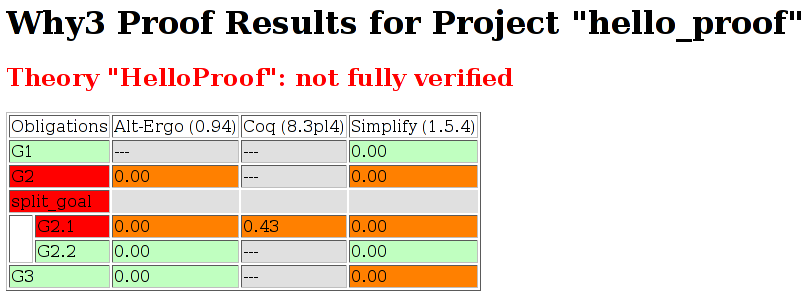
\includegraphics[width=0.9\textwidth]{hello_proof.png}}
  \end{center}
  \caption{HTML table produced for the HelloProof example}
\label{fig:html}
\end{figure}

The style 'table' outputs the contents of the session as a table,
similar to the LaTeX output above. Figure~\ref{fig:html} is the HTML
table produced for the 'HelloProof' example, as typically shown in a
Web browser. The gray cells filled with \texttt{---} just mean that
the prover was not run on the corresponding goal. Green background
means the result was ``Valid'', other cases are in orange
background. The red background for a goal means that the goal was not
proved.

The style ''simpletree' displays the contents of the session under the form of tree, similar to the tree view in the IDE. It uses only basic HTMl tags such as \verb|<ul>| and \verb|<li>|.

The style 'jstree' displays a dynamic tree view of the session, where
you can click on various parts to expand or shrink some part of the
tree. Clicking on a edited proof script also shows the contents of
this script. Technically, it use the 'jstree' plugin of the javascript
library 'jquery'.

Specific options for this command are as follows.
\begin{description}
\item[\texttt{-{}-style <s>}] sets the style to use, among
  \texttt{simpletree}, \texttt{jstree} and \texttt{table}, defaults to
  \texttt{table}.

\item[\texttt{-o}] the directory to output the produces files ('-' for
  stdout). The default is to output in the same directory as the session
  itself.

\item[\texttt{-{}-context}] adds context around the generated code in
  order to allow direct visualisation (header, css, ...). It also adds
  in the output directory all the needed external files. It can't be set with
  stdout output.

\item[\texttt{-{}-add\_pp <suffix> <cmd> <out\_suffix>}] adds for the
  given prefix the given pretty-printer, the new file as the given
  out\_suffix. cmd must contain '\%i' which will be replaced by the
  input file and '\%o' which will be replaced by the output file.

\item[\texttt{-{}-coqdoc}] use the \verb|coqdoc| command to display Coq proof
  scripts. This is equivalent to \texttt{-{}-add\_pp .v "coqdoc
    -{}-no-index -{}-html -o \%o \%i" .html}

\end{description}

\subsection{Commands modifying the proof attempts}

The subcommands \texttt{mod}, \texttt{copy}, \texttt{copy-archive},
and \texttt{rm} share the same set of options for selecting the proof
attempts to work on:
\begin{itemize}
\item Option \verb|--filter-prover| selects only the proof attempt with
  the given prover. This option can be specified multiple times to
  allow to select all the proofs that corresponds to one of the given
  provers. If this option is not specified, the proof are simply not
  filtered by there corresponding prover.
\item Option \verb|--filter-verified yes| restricts the selection to
  the proofs that are valid and not obsolete. On contrary the option
  \verb|--filter-verified no| select the ones that are not verified.
  \verb|--filter-verified all|, the default, does not select on this property.
\item Option \verb|--filter-verified-goal yes| restricts the selection
  to the proofs of verified goals (that does not mean that the proof is
  verified). Same for the other cases \verb|no| and \verb|all|.
\item Option \verb|--filter-archived yes| restricts the selection
  to the proofs that are archived.
  Same for the other cases \verb|no|
  and \verb|all| except the default is \verb|no|.
\end{itemize}

\noindent
The subcommand \texttt{mod}, \texttt{copy} and \texttt{copy-archive}
share the same set of option to specify the modification. The
subcommand \texttt{mod} modify directly the proof attempt,
\texttt{copy} copy the proof attempt before doing the modification,
\texttt{copy-archive} mark the original proof attempt as
archived.
The options are:
\begin{itemize}
\item Option \verb|--set-obsolete| marks the selected proofs as
  obsolete.
\item Option \verb|--set-archived| marks the selected proofs as archived.
\item Option \verb|--unset-archived| removes the archived attribute
  from the selected proofs.
\item Option \verb|--to-prover| modify the prover, for example
  \texttt{-{}-to-prover Alt-Ergo,0.94}. A conflict arises if a proof
  with this prover already exists. In this case you can choose between four
  behaviors:
\begin{itemize}
\item replace the proof (\verb|-f|, \verb|--force|);
\item do not replace the proof (\verb|-n|, \verb|--never|);
\item replace the proof unless it is verified (valid and not
  obsolete) (\verb|-c|, \verb|--conservative|); this is the default;
\item ask the user each time the case arises (\verb|-i|, \verb|--interactive|).
\end{itemize}
\end{itemize}


The subcommand \texttt{rm} removes the selected proof
attempts. The options \verb|-i, --interactive|, \verb|-f, --force| and
\verb|-c, --conservative| can also be used to respectively ask before
each suppression, suppress all the selected proof (default) and remove
only the proof that are not verified. The macro option \verb|--clean|
corresponds to \verb|--filter-verified-goal --conservative| and
removes the proof attempts that are not verified but which correspond
to verified goals.

The subcommands of this section don't accept by default to modify an
obsolete session (as defined in \ref{sec:idref:session}). You need to
add the option \verb|-F| to force this behavior.


% pour l'instant on ne documente pas parce que commenté dans le code
% \todo{A adapter en fonction de la decision sur l'upgrade de prover}

% If you just want to update one session with updated provers you can
% use \verb|--convert-unknown| instead of the option \verb|--to-prover|.
% \begin{verbatim}
% why3session copy  --convert-unknown
% \end{verbatim}
% For each proof attempt associated to an unknown prover (a prover not in
% \verb|.why3.conf|) and not archived, it will try to find a known prover
% with the same name. If it finds one, the proof attempt is copied to this
% prover and the old proof is set to archived. The corresponding edited
% files, if any, are copied and regenerated for the new prover An archived
% proof is not replayed by why3replayer.



\section{The \texttt{why3doc} tool}
\label{sec:why3doc}

This tool can produce HTML pages from \why source code. A source file
is scanned, \why code for theories or modules is output in
preformatted HTML code. Comments are interpreted in three different ways.
\begin{itemize}
\item Comments starting with at least three stars are completed
  ignored.
\item Comments starting with two stars are interpreted as textual
  documentation. Special constructs are interpreted as described
  below.
\item Comments starting with one star only are interpreted as code
  comments, and are typeset as the code
\end{itemize}

Additionally, all the \why identifiers are typeset with links so that
one can navigate through the HTML documentation, going from some
identifier use to its definition.

\paragraph{Options}

\begin{itemize}
\item Option \texttt{-o \textsl{<dir>}} defines the directory where to
  output the HTML files.
\item Option \verb|--output| is the same as \verb|-o|.
\item Option \verb|--index| (resp. \verb|--no-index|) to include
  (resp. exclude) the generation of an index file \texttt{index.html}.
  The default behavior is to generate an index if more than one file
  is passed on the command line.
\item Option \verb|--title|~\textsl{s} sets title \textsl{s} for the
  index page.
\item Option \verb|--stdlib-url|~\textsl{url} sets a URL for files
  found in load path, so that links to definitions can be added.
\end{itemize}

\paragraph{Typesetting textual comments}

Some constructs are interpreted:
\begin{itemize}
\item \texttt{\{\textsl{c text}\}} interprets character \textsl{c} as
  some typesetting command, detailed below
\item \texttt{[\textsl{code}]} is a code escape: the text
  \textsl{code} is typeset as \why code.
\end{itemize}

The typesetting commands are
\begin{description}
\item[1-6] a heading of level 1 to 6 respectively
\item[h] raw HTML
\end{description}

The HTML rendering is controlled via a CSS file \verb|style.css|
generated in the same directory as output files. This CSS style can be
modified manually: regenerating the doc will not overwrite an existing
\verb|style.css| file.



%%% Local Variables:
%%% mode: latex
%%% TeX-PDF-mode: t
%%% TeX-master: "manual"
%%% End:


\chapter{Language Reference}
\label{chap:syntaxref}

This chapter gives the grammar and semantics for \why and \whyml input files.

\section{Lexical conventions}

Lexical conventions are common to \why and \whyml.

% TODO: blanks

\paragraph{Comments.}
Comments are enclosed by \texttt{(*} and \texttt{*)} and can be nested.

\paragraph{Strings.}
Strings are enclosed in double quotes (\verb!"!). Double quotes can be
inserted in strings using the backslash character (\verb!\!).
In the following, strings are referred to with the non-terminal
\nonterm{string}{}.

% TODO: escape sequences for strings

\paragraph{Identifiers.} The syntax distinguishes lowercase and
uppercase identifiers and, similarly, lowercase and uppercase
qualified identifiers.

\begin{center}\framebox{\input{./qualid_bnf.tex}}\end{center}

\paragraph{Constants.}
The syntax for constants is given in Figure~\ref{fig:bnf:constant}.
Integer and real constants have arbitrary precision.
Integer constants may be given in base 16, 10, 8 or 2.
Real constants may be given in base 16 or 10.

\begin{figure}
\begin{center}\framebox{\input{./constant_bnf.tex}}\end{center}
  \caption{Syntax for constants.}
\label{fig:bnf:constant}
\end{figure}

\paragraph{Operators.}
Prefix and infix operators are built from characters organized in four
categories (\textsl{op-char-1} to \textsl{op-char-4}).
\begin{center}\framebox{\input{./operator_bnf.tex}}\end{center}
Infix operators are classified into 4 categories, according to the
characters they are built from:
\begin{itemize}
\item level 4: operators containing only characters from
\textit{op-char-4};
\item level 3: those containing
 characters from \textit{op-char-3} or \textit{op-char-4};
\item level 2: those containing
 characters from \textit{op-char-2}, \textit{op-char-3} or
 \textit{op-char-4};
\item level 1: all other operators (non-terminal \textit{infix-op-1}).
\end{itemize}

\paragraph{Labels.} Identifiers, terms, formulas, program expressions
can all be labeled, either with a string, or with a location tag.
\begin{center}\framebox{\input{./label_bnf.tex}}\end{center}
A location tag consists of a file name, a line number, and starting
and ending characters.

%%%%%%%%%%%%%%%%%%%%%%%%%%%%%%%%%%%%%%%%%%%%%%%%%%%%%%%%%%%%%%%%%%%%%%%%%%%%%%

\section{Why3 Language}

\paragraph{Terms.}
The syntax for terms is given in Figure~\ref{fig:bnf:term}.
The various constructs have the following priorities and
associativities, from lowest to greatest priority:
\begin{center}
  \begin{tabular}{|l|l|}
    \hline
    construct & associativity \\
    \hline\hline
    \texttt{if then else} / \texttt{let in} & -- \\
    label & -- \\
    cast  & -- \\
    infix-op level 1 & left \\
    infix-op level 2 & left \\
    infix-op level 3 & left \\
    infix-op level 4 & left \\
    prefix-op     & --   \\
    function application & left \\
    brackets / ternary brackets & -- \\
    bang-op       & --   \\
    \hline
  \end{tabular}
\end{center}

Note the curryfied syntax for function application, though partial
application is not allowed (rejected at typing).

\begin{figure}
  \begin{center}\framebox{\input{./term_bnf.tex}}\end{center}
  \caption{Syntax for terms.}
\label{fig:bnf:term}
\end{figure}

\paragraph{Type Expressions.} The syntax for type expressions is the following:
\begin{center}\framebox{\input{./type_bnf.tex}}\end{center}
Built-in types are \texttt{int}, \texttt{real}, and tuple types.
Note that the syntax for type
expressions notably differs from the usual ML syntax (\eg the
type of polymorphic lists is written \texttt{list 'a}, not \texttt{'a list}).

\paragraph{Formulas.}
The syntax for formulas is given Figure~\ref{fig:bnf:formula}.
The various constructs have the following priorities and
associativities, from lowest to greatest priority:
\begin{center}
  \begin{tabular}{|l|l|}
    \hline
    construct & associativity \\
    \hline\hline
    \texttt{if then else} / \texttt{let in} & -- \\
    label & -- \\
    \texttt{->} / \texttt{<->} & right \\
    \verb!\/! / \verb!||! & right \\
    \verb|/\| / \verb!&&! & right \\
    \texttt{not}  & -- \\
    infix level 1 & left \\
    infix level 2 & left \\
    infix level 3 & left \\
    infix level 4 & left \\
    prefix        & --   \\
    \hline
  \end{tabular}
\end{center}
Note that infix symbols of level 1 include equality (\texttt{=}) and
disequality (\texttt{<>}).

\begin{figure}
  \begin{center}\framebox{\input{./formula_bnf.tex}}\end{center}
  \caption{Syntax for formulas.}
\label{fig:bnf:formula}
\end{figure}

Notice that there are two symbols for the conjunction: \verb|/\|
and \verb|&&|, and similarly for disjunction. They are logically
equivalent, but may be treated slightly differently by some
transformations. For instance, \texttt{split} transforms the goal
\verb|A /\ B| into subgoals \verb|A| and \verb|B|, whereas it transforms
\verb|A && B| into subgoals \verb|A| and \verb|A -> B|. Similarly, it
transforms \verb!not (A || B)! into subgoals \verb|not A| and
\verb|not ((not A) /\ B)|.

\paragraph{Theories.}
The syntax for theories is given on Figure~\ref{fig:bnf:theorya} and~\ref{fig:bnf:theoryb}.

\begin{figure}
  \begin{center}\framebox{\input{./theory_bnf.tex}}\end{center}
  \caption{Syntax for theories (part 1).}
\label{fig:bnf:theorya}
\end{figure}

\begin{figure}
  \begin{center}\framebox{\input{./theory2_bnf.tex}}\end{center}
  \caption{Syntax for theories (part 2).}
\label{fig:bnf:theoryb}
\end{figure}

\paragraph{Files.}
A \why input file is a (possibly empty) list of theories.
\begin{center}\framebox{\input{./why_file_bnf.tex}}\end{center}


%%%%%%%%%%%%%%%%%%%%%%%%%%%%%%%%%%%%%%%%%%%%%%%%%%%%%%%%%%%%%%%%%%%%%%%%%%%%%%
\clearpage
\section{WhyML Language}\label{sec:syntax:whyml}

\subsection{Specification}

The syntax for specification clauses in programs 
is given in Figure~\ref{fig:bnf:spec}.
\begin{figure}
  \begin{center}\framebox{\input{./spec_bnf.tex}}\end{center}
  \caption{Specification clauses in programs.}
\label{fig:bnf:spec}
\end{figure}
Within specifications, terms are extended with new constructs
\verb|old| and \verb|at|:
\begin{center}\framebox{\input{./term_old_at_bnf.tex}}\end{center}
Within a postcondition, $\verb|old|~t$ refers to the value of term $t$
in the prestate. Within the scope of a code mark $L$,
the term $\verb|at|~t~\verb|'|L$ refers to the value of term $t$ at the program
point corresponding to $L$.

\subsection{Expressions}

The syntax for program expressions is given in
Figure~\ref{fig:bnf:expra} and~Figure~\ref{fig:bnf:exprb}.
\begin{figure}
  \begin{center}\framebox{\input{./expr_bnf.tex}}\end{center}
  \caption{Syntax for program expressions (part 1).}
\label{fig:bnf:expra}
\end{figure}

\begin{figure}
  \begin{center}\framebox{\input{./expr2_bnf.tex}}\end{center}
  \caption{Syntax for program expressions (part 2).}
\label{fig:bnf:exprb}
\end{figure}

In applications, arguments are evaluated from right to left.
This includes applications of infix operators, with the only exception of
lazy operators \verb|&&| and \verb+||+ that evaluate from left to
right, lazily.


% In the following we describe the informal semantics of each
% constructs, and provide the corresponding rule for computing the
% weakest precondition.


% \subsubsection{Constant Expressions, Unary and Binary Operators}


% Integer and real constants are as in the logic language, as weel as the unary and binary operators.


% \subsubsection{Array accesses and updates, fields access and updates}

% \todo{}

% \subsubsection{Let binding, sequences}

% \todo{}

% \subsubsection{Function definition}

% \todo{fun, let rec}

% \subsubsection{Function call}

% \todo{}

% \subsubsection{Exception throwing and catching}

% \todo{raise, try with end}

% \subsubsection{Conditional expression, pattern matching}

% \todo{if then else. Discuss standard WP versus fast WP}

% \subsubsection{Iteration Expressions}

% There are three kind of expressions for iterating: bounded, unbounded and infinite.

% \begin{itemize}
% \item A bounded iteration has the form
% \begin{flushleft}\ttfamily
%   for $i$=$a$ to $b$ do invariant \{ $I$ \} $e$ done
% \end{flushleft}
% Expressions $a$ and $b$ are evaluated first and only once, then expression $e$ si evaluated successively for $i$ from $a$ to $b$ included. Nothing is executed if $a > b$. The invariant $I$ must hold at each iteration including before entering the loop and when leaving it. The rule for computing WP is as follows:
% \begin{eqnarray*}
%   WP(\texttt{for} \ldots, Q) &=& I(a) \land \\
% && \forall \vec{w} (\forall i, a \leq i \leq b \land I(i) \rightarrow WP(e,I(i+1))) \land (I(b+1) \rightarrow Q)
% \end{eqnarray*}
% where $\vec{w}$ is the set of references modified by $e$.

% A downward bounded iteration is also available, under the form
% \begin{flushleft}\ttfamily
%   for $i$=$a$ downto $b$ do invariant \{ $I$ \} $e$ done
% \end{flushleft}

% \item An unbounded iteration has the form
% \begin{flushleft}\ttfamily
%   while $c$ do invariant \{ $I$ \} $e$ done
% \end{flushleft}
% it iterates the loop body $e$ until the condition $c$ becomes false. 
% \begin{eqnarray*}
%   WP(\texttt{while} \ldots, Q) &=& I \land \\
% && \forall \vec{w} (c \land I \rightarrow WP(e,I)) \land (\neg c \land I \rightarrow Q)
% \end{eqnarray*}
% where $\vec{w}$ is the set of references modified by $e$.

% Additionally, such a loop can be given a variant $v$, a quantity that must decreases ar each iteration, so as to prove its termination.


% \item An infinite iteration has the form
% \begin{flushleft}\ttfamily
%   loop invariant \{ $I$ \} $e$ end
% \end{flushleft}
% it iterates the loop forever, hence the only way to exit such a loop is to raise an exception.
% \begin{eqnarray*}
%   WP(\texttt{loop} \ldots, Q \mid Exc \Rightarrow R) &=& I \land \\
% && \forall \vec{w} (I \rightarrow WP(e,I)) \land (I \rightarrow WP(e,Exc \Rightarrow R))
% \end{eqnarray*}
% \end{itemize}

% \subsubsection{Assertions, Code Contracts}

% There are several form of expressions for inserting annotations in the code.
% The first form of those are the \emph{assertions} which have the form
% \begin{flushleft}\ttfamily
%   \textsl{keyword} \{ \textsl{proposition} \}
% \end{flushleft}
% where \textsl{keyword} is either \texttt{assert}, \texttt{assume} or
% \texttt{check}. They all state that the given proposition holds at the given program point. The differences are:
% \begin{itemize}
% \item \texttt{assert} requires to prove that the proposition holds, and then make it available in the context of the remaining of the code
% \item \texttt{check} requires to prove that the proposition holds, but
%   does not make it visible in the remaining
% \item \texttt{assume} assumes that the proposition holds and make it
%   visible in the context of the remaining code, without requiring to
%   prove it. It acts like an axiom, but within a program.
% \end{itemize}
% The corresponding rules for computing WP are as follows:
% \begin{eqnarray*}
%   WP(\texttt{assert} \{ P \}, Q) &=& P \mathop{\&\&} Q = P \land (P \rightarrow Q)\\
%   WP(\texttt{check} \{ P \}, Q) &=& P \land Q \\
%   WP(\texttt{assume} \{ P \}, Q) &=& P \rightarrow Q
% \end{eqnarray*}

% The other forms of code contracts allow to abstract a piece of code by specifications.
% \begin{itemize}
% \item $\texttt{any}~\{ P \}~\tau~\epsilon~\{ Q \}$ is a
%   non-deterministic expression that requires the precondition $P$ to
%   hold, then makes some side effects $\epsilon$, and returns any value
%   of type $\tau$ such that $Q$ holds. This construct acts as an axiom
%   in the sense that it does not check whether there exists any program
%   that can effectively establish the post-condition (similarly as the
%   introduction of a \texttt{val} at the global level).
% \item $\texttt{abstract}~e~\{ Q \}$ makes sure that the evaluation of
%   expression $e$ establishes the post-condition $Q$, and then abstract
%   away the program state by the post-condition $Q$ (similarly to the
%   \texttt{any} construct).
% \end{itemize}
% The corresponding rules for computing WP are as follows:
% \[
% \begin{array}{l}
%   WP(\texttt{any}~\{ P \}~\tau~\epsilon~\{ Q \mid exn_i \Rightarrow R_i \} ,
%   Q'  exn_i \Rightarrow R'_i) = \\
%   \qquad\qquad P \mathop{\&\&} \forall result, \epsilon.
%   (Q \rightarrow Q') \land (R_i \rightarrow R'_i) \\
%   WP(\texttt{abstract}~e~\{ Q \mid exn_i \Rightarrow R_i \} ,
%   Q' \mid exn_i \Rightarrow R'_i) = \\
%   \qquad\qquad WP(e,Q \mid exn_i \Rightarrow R_i) \land
%   \forall result, \epsilon, Q \rightarrow Q' \land R_i \rightarrow R'_i
% \end{array}
% \]

% \subsubsection{Labels, Operators \texttt{old} and \texttt{at}}

% \todo{Labels, old, at}

\subsection{Modules}

The syntax for modules is given in Figure~\ref{fig:bnf:module}.
\begin{figure}
  \begin{center}\framebox{\input{./module_bnf.tex}}\end{center}
  \caption{Syntax for modules.}
\label{fig:bnf:module}
\end{figure}
Any declaration which is accepted in a theory is also accepted in a
module. Additionally, modules can introduce record types with mutable
fields and declarations which are specific to programs (global
variables, functions, exceptions).

\subsection{Files}

A \whyml input file is a (possibly empty) list of theories and modules.
\begin{center}\framebox{\input{./whyml_file_bnf.tex}}\end{center}
A theory defined in a \whyml\ file can only be used within that
file. If a theory is supposed to be reused from other files, be they
\why\ or \whyml\ files, it should be defined in a \why\ file.


%%% Local Variables:
%%% mode: latex
%%% TeX-PDF-mode: t
%%% TeX-master: "manual"
%%% End:


\chapter{Standard Library}
\label{chap:library}

This chapter provides a short description of the contents of \why
standard library. It contains both standard logic theories, described
in Section~\ref{sec:stdlib}, and standard ML modules, described in
Section~\ref{sec:mllibrary}.

Only a rough introduction of the theories and modules is given
here. For detailed information, one should refer to the on-line
documentation automatically generated from the actual sources,
available at \url{http://why3.lri.fr/stdlib/}.


\section{Theories}
\label{sec:stdlib}

We present the most important theories here, see the URL above for the
others.

Notice there is an alternative way to explore the contents of a
library, using the \verb|why3| command with option 
\verb|-T| and a qualified theory name, for example:
\index{theory@\verb+--theory+}

\begin{verbatim}
> why3 -T bool.Ite
theory Ite
  (* use BuiltIn *)

  (* use Bool *)

  function ite (b:bool) (x:'a) (y:'a) : 'a =
    match b with
    | True -> x
    | False -> y
    end
end
\end{verbatim}

In the following, for each library, we describe the main theories
defined in it.

\subsection{Library \texttt{bool}}

\begin{description}

\item[Bool] provides the Boolean data type \verb|bool| with
  constructors \verb|True| and \verb|False|; and operations \verb|andb|, \verb|orb|, \verb|xorb|, \verb|notb|.
\indextt{bool}
\indextt{True}
\indextt{False}

\item[Ite] provides the polymorphic if-then-else operator written as \verb|ite|.

\end{description}

\subsection{Library \texttt{int}}

\begin{description}

\item[Int] provides the basic operations \verb|+|, \verb|-|, and
  \verb|*|, and the comparison operators \verb|<|, \verb|>|, \verb|>=|, and
  \verb|<=|.

\item[Abs] provides the absolute value written as \verb|abs|.

\item[EuclideanDivision] defines division and modulo, where division rounds
  down, written as \verb|div| and \verb|mod|.

\item[ComputerDivision] defines division and modulo, where division rounds to
  zero, also written as \verb|div| and \verb|mod|.

\item[MinMax] provides \verb|min| and \verb|max| operators.

\end{description}

See the on-line web documentation for the other theories defined in the
\texttt{int} library.

\subsection{Library \texttt{real}}

\begin{description}

\item[Real] provides basic operations \verb|+|, \verb|-|, \verb|*| and \verb|/|;
  comparison operators.

\item[RealInfix] provides basic operations with alternative syntax \verb|+.|,
  \verb|-.|, \verb|*.|, \verb|/.|, \verb|<.|, \verb|>.|, \verb|<=.|, and \verb|>=.|, to
  allow simultaneous use of integer and real operators.

\item[Abs] provides absolute value written as \verb|abs|.

\item[MinMax] provides \verb|min| and \verb|max| operators.

\item[FromInt] provides the operator \verb|from_int| to convert an integer to a real.

\item[Truncate] provides conversion operators from real to integers:
  \verb|truncate| rounds to 0, \verb|floor| rounds down, and
  \verb|ceil| rounds up.

\item[Square] provides operators \verb|sqr| and \verb|sqrt| for square and square root.

% \item[ExpLog] functions \verb|exp|, \verb|log|, \verb|log2|, and \verb|log10|.

% \item[PowerReal] function \verb|pow| with two real parameters.

% \item[PowerInt] function \verb|pow| with integer only exponents.

% \item[Trigonometry] functions \verb|cos|, \verb|sin|, \verb|tan|, and
%   \verb|atan|. Constant \verb|pi|.

% \item[Hyperbolic] functions \verb|cosh|, \verb|sinh|, \verb|tanh|,
%   \verb|acosh|, \verb|asinh|, \verb|atanh|.

% \item[Polar] functions \verb|hypot| and \verb|atan2|.

\end{description}

See the on-line web documentation for the other theories defined in the
\texttt{real} library, such exponential, logarithm, power,
trigonometric functions.

\subsection{Library \texttt{floating\_point}}

This library provides a theory of IEEE-754 floating-point numbers. It
is inspired by~\cite{ayad10ijcar}.

\subsection{Library \texttt{map}}

This library provides the data type of purely applicative maps. It is
polymorphic both in the index type and the contents. There are also a
few theories and operators specialized to maps indexed by integers,
such as the sorted predicate, permutation, etc.

\subsection{Library \texttt{option}}

This library provides the classical ML option type with constructors
\verb|None| and \verb|Some|.
\indextt{None}
\indextt{Some}

\subsection{Library \texttt{list}}

This library provides the classical ML type of polymorphic lists, with
constructors \verb|Nil| and \verb|Cons|. Most of the classical list
operators are provided in separate theories.

\section{Modules}
\label{sec:mllibrary}

The standard ML modules provided allow to write imperative
programs. The two main modules are the one providing ML references,
and the one providing arrays.

\subsection{Library \texttt{ref}}


\begin{description}
\item[Ref] provides references \emph{i.e.} mutable variables:
  type \verb|ref 'a| and functions \verb|ref| for creation,
  \verb|(!)| for access, and \verb|(:=)| for mutation.
\item[Refint] provides additional functions \texttt{incr},
  \texttt{decr} and a few others, over integer references.
\end{description}
\indextt{ref}
\index{"!@\texttt{"!}}
\indextt{:=}

\subsection{Library \texttt{array}}

\begin{description}
\item[Array]polymorphic arrays (type \texttt{array 'a}, infix
  syntax $a[i]$ for access and $a[i] \leftarrow e$ for update,
  functions \texttt{length}, \texttt{make}, \texttt{append},
  \texttt{sub}, \texttt{copy}, \texttt{fill}, and \texttt{blit})
\item[ArraySorted] an array of integers is sorted
  (\verb|array_sorted_sub| and \verb|array_sorted|)
\item[ArrayEq] two arrays are identical
  (\verb|array_eq_sub| and \verb|array_eq|)
\item[ArrayPermut] two arrays are permutation of each other
  (\verb|permut_sub| and \verb|permut|)
\end{description}

\subsection{Standard Data Types}

A few other classical data types are provided, such as queues (library
\texttt{queue}), stacks (library \texttt{stack}), hash tables (library
\texttt{hashtbl}), characters and strings (library \texttt{string}),
etc.


%%% Local Variables:
%%% mode: latex
%%% TeX-PDF-mode: t
%%% TeX-master: "manual"
%%% End:


\chapter{Theory realizations}
\label{chap:realizations}

\section{Generating a realization}

Generating the skeleton for a theory is done by passing to \why the
\verb+--realize+ option, a driver suitable for realizations, the names of
the theories to realize, and the target directory.

\begin{verbatim}
\why3 --realize -D path/to/drivers/coq-realize.drv
      -T env_path.theory_name -o path/to/target/dir/
\end{verbatim}

The name of the generated file is inferred from the theory name. If the
target directory already contains a file with the same name, \why
extracts all the parts that it assumes to be user-made and prints them in
the generated file.

\section{Using realizations inside proofs}

If a theory has been realized, a \why printer for an interactive prover
will no longer output assumptions from the theory but instead simply put
a directive to load the realization. In order to indicate to the printer
that a given theory is realized, one has to add a meta declaration to the
corresponding theory section.

\begin{verbatim}
theory env_path.theory_name
  meta "realized" "env_path.theory_name", "optional_naming"
end
\end{verbatim}

The first parameter is the theory name for \why, while the second
parameter, if not empty, provides a name to be used inside generated
scripts to point to the realization, in case the default name is not
suitable for the interactive prover.

\section{Coq scripts}

This section describes the content of the Coq files generated by \why for
both proof obligations and theory realizations. When reading a Coq
script, \why is guided by the presence of empty lines to split the
script, so the user should refrain from removing empty lines around
generated parts or adding empty lines inside them.

\begin{enumerate}
\item	The header of the file contains all the library inclusions
	required by the driver file. Any user-made changes to this part
	will be lost when the file is regenerated by \why. This part ends
	at the first empty line.
\item	Abstract logic symbols are assumed with the vernacular directive
	\verb+Paramater+. Axioms are assumed with the \verb+Axiom+
	directive. When regenerating a script, \why assumes that all such
	symbols have been generated by a previous run. As a consequence,
	the user should not introduce new symbols with these two
	directives, as they would be lost.
\item	Definitions of functions and inductive types in theories are
	printed in a block that starts with \verb+(* Why3 assumption *)+.
	This comment should not be removed; otherwise \why will assume
	that the definition is user-made.
\item	Finally, proof obligations and symbols to be realized are
	introduced by \verb+(* Why3 goal *)+. The user is supposed to
	fill the script after the statement. \why assumes that the
	user-made part extends up to \verb+Qed+, \verb+Admitted+,
	\verb+Save+, or \verb+Defined+, whichever comes first. In the
	case of definitions, the original statement can be replaced by
	a \verb+Notation+ directive, in order to ease the usage of
	already defined symbols.
\end{enumerate}

Currently, the parser for Coq scripts is rather naive and does not know
much about comments. For instance, \why can easily be confused by
some terminating directive like \verb+Qed+ that would be present in a
comment.

\section{Shipping libraries of realizations}

While modifying an existing driver file might be sufficient for local
use, it does not scale well when the realizations are to be shipped to
other users. Instead, an additional configuration file should be created.

\begin{verbatim}
[main]
loadpath="path/to/theories"

[prover coq]
option="-R path/to/vo/files Logical_directory"
driver="path/to/extra_coq.drv"
\end{verbatim}

This file can be passed to \why thanks to the \verb+--extra-config+
option.


\chapter{Coq Tactic}
\label{chap:tactic}
\index{Coq proof assistant}

\why\ provides a Coq tactic to call external theorem provers as oracles.

\section{Installation}

You need Coq version 8.3 or greater. If this is the case, \why's
configuration detects it, then compiles and installs the Coq tactic.
The Coq tactic is installed in
\begin{center}
  \textit{why3-lib-dir}\texttt{/coq-tactic/}
\end{center}
where \textit{why3-lib-dir} is \why's library directory, as reported
by \verb+why3 --print-libdir+. This directory
is automatically added to Coq's load path if you are
calling Coq via \why (from \texttt{why3ide}, \texttt{why3replayer},
etc.). If you are calling Coq by yourself, you need to add
this directory to Coq's load path, either using Coq's command line
option \texttt{-I} or by adding
\begin{center}
  \verb+Add LoadPath "+\textit{why3-lib-dir}\verb+/coq-tactic/".+
\end{center}
to your \texttt{\~{}/.coqrc} resource file.

\section{Usage}

The Coq tactic is called \texttt{why3} and is used as follows:
\begin{center}
  \texttt{why3} \verb+"+\textit{prover-name}\verb+"+
  $[$\texttt{timelimit} \textit{n}$]$.
\end{center}
The string \textit{prover-name} identifies one of the automated theorem provers
supported by \why, as reported by \verb+why3 --list-provers+
(interactive provers excluded).
The current goal is then translated to \why's logic and the prover is
called. If it reports the goal to be valid, then Coq's \texttt{admit}
tactic is used to assume the goal. The prover is called with a time
limit in seconds as given by \why's configuration file
(see page~\pageref{sec:whyconffile}). A different value may be given
using the \texttt{timelimit} keyword.

\paragraph{Error messages.} The following errors may be reported by
the Coq tactic.
\begin{description}
\item[\texttt{Not a first order goal}]\emptyitem
  The Coq goal could not be translated to \why's logic.
\item[\texttt{Timeout}]\emptyitem
  There was no answer from the prover within the given time limit.
\item[\texttt{Don't know}]\emptyitem
  The prover stopped without validating the goal.
\item[\texttt{Invalid}]\emptyitem
  The prover stopped, reporting the goal to be invalid.
\item[\texttt{Failure}]\emptyitem
  The prover failed. Depending on the message that follows, you may
  want to file a bug report, either to the \why\ developers or to the
  prover developers.
\end{description}

%%% Local Variables:
%%% mode: latex
%%% compile-command: "make -C .. doc"
%%% TeX-PDF-mode: t
%%% TeX-master: "manual"
%%% End:


% \chapter{Complete API documentation} *)
% \label{chap:apidoc} *)

% \input{./apidoc.tex} *)

% \appendix

\chapter{Technical Informations}
%HEVEA\cutname{technical.html}

\section{Structure of Session Files}

The proof session state is stored in an XML file named
\texttt{\textsl{<dir>}/why3session.xml}, where \texttt{\textsl{<dir>}}
is the directory of the project.
The XML file follows the DTD given in \texttt{share/why3session.dtd} and reproduced below.
\lstinputlisting{../share/why3session.dtd}


\section{Prover Detection}
\label{sec:proverdetecttiondata}

The data configuration for the automatic detection of
installed provers is stored in the file
\texttt{provers-detection-data.conf} typically located in directory
\verb|/usr/local/share/why3| after installation. The content of this
file is reproduced below.
%BEGIN LATEX
{\footnotesize
%END LATEX
\lstinputlisting[language={},morecomment={[l]\#},morestring={[b]"}]{../share/provers-detection-data.conf}
%BEGIN LATEX
}
%END LATEX

\section{The \texttt{why3.conf} Configuration File}
\label{sec:whyconffile}
\index{why3.conf@\texttt{why3.conf}}\index{configuration file}

One can use a custom configuration file. The \why
tools look for it in the following order:
\begin{enumerate}
\item the file specified by the \texttt{-C} or \texttt{-{}-config} options,
\item the file specified by the environment variable
  \texttt{WHY3CONFIG} if set,
\item the file \texttt{\$HOME/.why3.conf}
  (\texttt{\$USERPROFILE/.why3.conf} under Windows) or, in the case of
  local installation, \texttt{why3.conf} in the top directory of \why sources.
\end{enumerate}
If none of these files exist, a built-in default configuration is used.

A section begins with a header inside square brackets and ends at the
beginning of the next section. The header of a section can be a single
identifier, \eg \texttt{[main]}, or it can be composed by a family name
and a single family argument, \eg \texttt{[prover alt-ergo]}.

Sections contain associations \texttt{key=value}. A value is either
an integer (\eg \texttt{-555}), a boolean (\texttt{true}, \texttt{false}),
or a string (\eg \texttt{"emacs"}). Some specific keys can be attributed
multiple values and are
thus allowed to occur several times inside a given section. In that
case, the relative order of these associations matters.

\section{Drivers for External Provers}
\label{sec:drivers}

Drivers for external provers are readable files located in the
\texttt{drivers} directory. They describe how \why should interact
with external provers.

% Experienced users can modify them to
% change the way \why interacts with external provers.

%  namely the need
% for printer section, any other ?

% , in particular which transformations
% are applied to goals.


Files with \texttt{.drv} extension represent drivers that might be
associated to a specific solver in the \texttt{why3.conf}
configuration file (see \ref{sec:whyconffile} for more information);
files with \texttt{.gen} extension are intended to be imported by
other drivers; finally, files with \texttt{.aux} extension are
automatically generated from the main \texttt{Makefile}.
%
\input{./generated/drivers_dependency.tex}
%
The most important drivers dependencies are shown in
Figs.~\driversref. Fig.~\ref{fig:drv:smt} shows the drivers files
related to the \texttt{SMT} solvers, Fig.~\ref{fig:drv:coq} the files
for \texttt{Coq}, Fig.~\ref{fig:drv:tptp} the files for \texttt{TPTP},
Fig.~\ref{fig:drv:isabelle} the files for \texttt{Isabelle}, and
finally Fig.~\ref{fig:drv:pvs} shows the files for \texttt{PVS}.

\section{Transformations}
\label{sec:transformations}

This section documents the available transformations. We first
describe the most important ones, and then we provide a quick
documentation of the others, first the non-splitting ones, \eg those
which produce exactly one goal as result, and the others which produce any
number of goals.

Notice that the set of available transformations in your own
installation is given by
\begin{verbatim}
why3 --list-transforms
\end{verbatim}
\index{list-transforms@\verb+--list-transforms+}

\subsection{Inlining definitions}

Those transformations generally amount to replace some applications of
function or predicate symbols with its definition.

\begin{description}

\item[inline\_trivial]
  expands and removes definitions of the form
\begin{whycode}
function  f x_1 ... x_n = (g e_1 ... e_k)
predicate p x_1 ... x_n = (q e_1 ... e_k)
\end{whycode}
when each $e_i$ is either a ground term or one of the $x_j$, and
each $x_1 \dots x_n$ occurs at most once in all the $e_i$.

The attribute \texttt{[@inline:trivial]} is used to tag functions that
the transformation will force expand (not using the conditions above). This can
be used to ensure that some specific functions are inlined for automatic
provers (inline\_trivial is used in many drivers).

\index{inline-trivial@\verb+inline_trivial+}

\item[inline\_goal] expands all outermost symbols of the goal that
  have a non-recursive definition.
\index{inline-goal@\verb+inline_goal+}

\item[inline\_all]
  expands all non-recursive definitions.
\index{inline-all@\verb+inline_all+}

\end{description}


\subsection{Induction Transformations}

\begin{description}
\item[induction\_ty\_lex]
  \index{induction-ty-lex@\verb+induction_ty_lex+}
  performs structural, lexicographic induction on
  goals involving universally quantified variables of algebraic data
  types, such as lists, trees, etc. For instance, it transforms the
  following goal
\begin{whycode}
goal G: forall l: list 'a. length l >= 0
\end{whycode}
  into this one:
\begin{whycode}
goal G :
  forall l:list 'a.
     match l with
     | Nil -> length l >= 0
     | Cons a l1 -> length l1 >= 0 -> length l >= 0
     end
\end{whycode}
  When induction can be applied to several variables, the transformation
  picks one heuristically. The \verb|[@induction]| attribute can be used to
  force induction over one particular variable, \eg with
\begin{whycode}
goal G: forall l1 [@induction] l2 l3: list 'a.
        l1 ++ (l2 ++ l3) = (l1 ++ l2) ++ l3
\end{whycode}
induction will be applied on \verb|l1|. If this attribute is attached to
several variables, a lexicographic induction is performed on these
variables, from left to right.

%\item[] Induction on inductive predicates.

%[TO BE COMPLETED]

% TODO: implement also induction on int !

\end{description}

\subsection{Simplification by Computation}

These transformations simplify the goal by applying several kinds of
simplification, described below. The transformations differ only by
the kind of rules they apply:
\begin{description}
\item[compute\_in\_goal] aggressively applies all known
  computation/simplification rules.
  \index{compute-in-goal@\verb+compute_in_goal+}

\item[compute\_specified] performs rewriting using only built-in
  operators and user-provided rules.
  \index{compute-specified@\verb+compute_specified+}
\end{description}

The kinds of simplification are as follows.
\begin{itemize}
\item Computations with built-in symbols, \eg operations on integers,
  when applied to explicit constants, are evaluated. This includes
  evaluation of equality when a decision can be made (on integer
  constants, on constructors of algebraic data types), Boolean
  evaluation, simplification of pattern-matching/conditional expression,
  extraction of record fields, and beta-reduction.
  At best, these computations reduce the goal to
  \verb|true| and the transformations thus does not produce any sub-goal.
  For example, a goal
  like \verb|6*7=42| is solved by those transformations.
\item Unfolding of definitions, as done by \verb|inline_goal|. Transformation
  \verb|compute_in_goal| unfolds all definitions, including recursive ones.
  For \verb|compute_specified|, the user can enable unfolding of a specific
  logic symbol by attaching the meta \verb|rewrite_def| to the symbol.
\begin{whycode}
function sqr (x:int) : int = x * x
meta "rewrite_def" function sqr
\end{whycode}
\item Rewriting using axioms or lemmas declared as rewrite rules. When
  an axiom (or a lemma) has one of the forms
\begin{whycode}
axiom a: forall ... t1 = t2
\end{whycode}
  or
\begin{whycode}
axiom a: forall ... f1 <-> f2
\end{whycode}
  then the user can declare
\begin{whycode}
meta "rewrite" prop a
\end{whycode}
  to turn this axiom into a rewrite rule. Rewriting is always done
  from left to right. Beware that there is no check for termination
  nor for confluence of the set of rewrite rules declared.
\end{itemize}
Instead of using a meta, it is possible to declare an axiom as a
rewrite rule by adding the \verb|[@rewrite]| attribute on the axiom name or
on the axiom itself, e.g.:
\begin{whycode}
axiom a [@rewrite]: forall ... t1 = t2
lemma b: [@rewrite] forall ... f1 <-> f2
\end{whycode}
The second form allows some form of local rewriting, e.g.
\begin{whycode}
lemma l: forall x y. ([@rewrite] x = y) -> f x = f y
\end{whycode}
can be proved by \verb|introduce_premises| followed by \verb|compute_specified|.

\paragraph{Bound on the number of reductions}
The computations performed by these transformations can take an
arbitrarily large number of steps, or even not terminate. For this
reason, the number of steps is bounded by a maximal value, which is
set by default to 1000. This value can be increased by another meta,
\eg
\begin{whycode}
meta "compute_max_steps" 1_000_000
\end{whycode}
When this upper limit is reached, a warning is issued, and the
partly-reduced goal is returned as the result of the transformation.


\subsection{Other Non-Splitting Transformations}

\begin{description}

\item[eliminate\_algebraic] replaces algebraic data types by first-order
definitions~\cite{paskevich09rr}.
\index{eliminate-algebraic@\verb+eliminate_algebraic+}

\item[eliminate\_builtin] removes definitions of symbols that are
  declared as builtin in the driver, \ie with a ``syntax'' rule.
\index{eliminate-builtin@\verb+eliminate_builtin+}

\item[eliminate\_definition\_func]
  replaces all function definitions with axioms.
\index{eliminate-definition-func@\verb+eliminate_definition_func+}

\item[eliminate\_definition\_pred]
  replaces all predicate definitions with axioms.
\index{eliminate-definition-pred@\verb+eliminate_definition_pred+}

\item[eliminate\_definition]
  applies both transformations above.
\index{eliminate-definition@\verb+eliminate_definition+}

\item[eliminate\_mutual\_recursion]
  replaces mutually recursive definitions with axioms.
\index{eliminate-mutual-recursion@\verb+eliminate_mutual_recursion+}

\item[eliminate\_recursion]
  replaces all recursive definitions with axioms.
\index{eliminate-recursion@\verb+eliminate_recursion+}

\item[eliminate\_if\_term] replaces terms of the form \texttt{if
    formula then t2 else t3} by lifting them at the level of formulas.
  This may introduce \texttt{if then else} in formulas.
\index{eliminate-if-term@\verb+eliminate_if_term+}

\item[eliminate\_if\_fmla] replaces formulas of the form \texttt{if f1 then f2
  else f3} by an equivalent formula using implications and other
  connectives.
\index{eliminate-if-fmla@\verb+eliminate_if_fmla+}

\item[eliminate\_if]
  applies both transformations above.
\index{eliminate-if@\verb+eliminate_if+}

\item[eliminate\_inductive] replaces inductive predicates by
  (incomplete) axiomatic definitions, \ie construction axioms and
  an inversion axiom.
\index{eliminate-inductive@\verb+eliminate_inductive+}

\item[eliminate\_let\_fmla]
  eliminates \texttt{let} by substitution, at the predicate level.
\index{eliminate-let-fmla@\verb+eliminate_let_fmla+}

\item[eliminate\_let\_term]
  eliminates \texttt{let} by substitution, at the term level.
\index{eliminate-let-term@\verb+eliminate_let_term+}

\item[eliminate\_let]
  applies both transformations above.
\index{eliminate-let@\verb+eliminate_let+}

% \item[encoding\_decorate\_mono]

% \item[encoding\_enumeration]

\item[encoding\_smt]
  encodes polymorphic types into monomorphic types~\cite{conchon08smt}.
\index{encoding-smt@\verb+encoding_smt+}

\item[encoding\_tptp]
  encodes theories into unsorted logic. %~\cite{cruanes10}.
\index{encoding-tptp@\verb+encoding_tptp+}

% \item[filter\_trigger] *)

% \item[filter\_trigger\_builtin] *)

% \item[filter\_trigger\_no\_predicate] *)

% \item[hypothesis\_selection] *)
%   Filter hypothesis of goals~\cite{couchot07ftp,cruanes10}. *)

\item[introduce\_premises] moves antecedents of implications and
  universal quantifications of the goal into the premises of the task.
\index{introduce-premises@\verb+introduce_premises+}

% \item[remove\_triggers] *)
%   removes the triggers in all quantifications. *)

\item[simplify\_array] automatically rewrites the task using the lemma
  \verb|Select_eq| of theory \verb|map.Map|.
\index{simplify-array@\verb+simplify_array+}

\item[simplify\_formula] reduces trivial equalities $t=t$ to true and
  then simplifies propositional structure: removes true, false, simplifies
  $f \land f$ to $f$, etc.
\index{simplify-formula@\verb+simplify_formula+}

\item[simplify\_recursive\_definition] reduces mutually recursive
  definitions if they are not really mutually recursive, \eg
\begin{whycode}
function f : ... = ... g ...
with g : ... = e
\end{whycode}
becomes
\begin{whycode}
function g : ... = e
function f : ... = ... g ...
\end{whycode}
if $f$ does not occur in $e$.
\index{simplify-recursive-definition@\verb+simplify_recursive_definition+}

\item[simplify\_trivial\_quantification]
  simplifies quantifications of the form
\begin{whycode}
forall x, x = t -> P(x)
\end{whycode}
into
\begin{whycode}
P(t)
\end{whycode}
  when $x$ does not occur in $t$.
  More generally, this simplification is applied whenever $x=t$ or
  $t=x$ appears in negative position.
\index{simplify-trivial-quantification@\verb+simplify_trivial_quantification+}

\item[simplify\_trivial\_quantification\_in\_goal]
  is the same as above but it applies only in the goal.
\index{simplify-trivial-quantification-in-goal@\verb+simplify_trivial_quantification_in_goal+}

\item[split\_premise] replaces axioms in conjunctive form
  by an equivalent collection of axioms.
  In absence of case analysis attributes (see \texttt{split\_goal} for details),
  the number of axiom generated per initial axiom is
  linear in the size of that initial axiom.
\index{split-premise@\verb+split_premise+}

\item[split\_premise\_full] is similar to \texttt{split\_premise}, but it
  also converts the axioms to conjunctive normal form. The number of
  axioms generated per initial axiom may be exponential in the size of
  the initial axiom.
\index{split-premise-full@\verb+split_premise_full+}

\end{description}

\subsection{Other Splitting Transformations}
\label{tech:trans:split}

\begin{description}

\item[simplify\_formula\_and\_task] is the same as \texttt{simplify\_formula}
  but it also removes the goal if it is equivalent to true.
\index{simplify-formula-and-task@\verb+simplify_formula_and_task+}

\item[split\_goal] changes conjunctive goals into the
  corresponding set of subgoals. In absence of case analysis attributes,
  the number of subgoals generated is linear in the size of the initial goal.

  \paragraph{Behavior on asymmetric connectives and
    \texttt{by}/\texttt{so}}

  The transformation treats specially asymmetric and
  \texttt{by}/\texttt{so} connectives. Asymmetric conjunction
  \verb|A && B| in goal position is handled as syntactic sugar for
  \verb|A /\ (A -> B)|.  The conclusion of the first subgoal can then
  be used to prove the second one.

  Asymmetric disjunction \verb+A || B+ in hypothesis position is handled as
  syntactic sugar for \verb|A \/ ((not A) /\ B)|.
  In particular, a case analysis on such hypothesis would give the negation of
  the first hypothesis in the second case.

  The \texttt{by} connective is treated as a proof indication. In
  hypothesis position, \verb|A by B| is treated as if it were
  syntactic sugar for its regular interpretation \verb|A|. In goal
  position, it is treated as if \verb|B| was an intermediate step for
  proving \verb|A|. \verb|A by B| is then replaced by \verb|B| and the
  transformation also generates a side-condition subgoal \verb|B -> A|
  representing the logical cut.

  Although splitting stops at disjunctive points like symmetric
  disjunction and left-hand sides of implications, the occurrences of
  the \texttt{by} connective are not restricted. For instance:
  \begin{itemize}
  \item Splitting
\begin{whycode}
goal G : (A by B) && C
\end{whycode}
generates the subgoals
\begin{whycode}
goal G1 : B
goal G2 : A -> C
goal G3 : B -> A (* side-condition *)
\end{whycode}
\item Splitting
\begin{whycode}
goal G : (A by B) \/ (C by D)
\end{whycode}
generates
\begin{whycode}
goal G1 : B \/ D
goal G2 : B -> A (* side-condition *)
goal G3 : D -> C (* side-condition *)
\end{whycode}
\item Splitting
\begin{whycode}
goal G : (A by B) || (C by D)
\end{whycode}
generates
\begin{whycode}
goal G1 : B || D
goal G2 : B -> A        (* side-condition *)
goal G3 : B || (D -> C) (* side-condition *)
\end{whycode}
Note that due to the asymmetric disjunction, the disjunction is kept in the
second side-condition subgoal.
\item Splitting
\begin{whycode}
goal G : exists x. P x by x = 42
\end{whycode}
generates
\begin{whycode}
goal G1 : exists x. x = 42
goal G2 : forall x. x = 42 -> P x (* side-condition *)
\end{whycode}
Note that in the side-condition subgoal, the context is universally closed.
\end{itemize}

The \texttt{so} connective plays a similar role in hypothesis position, as it serves as a consequence indication. In goal position, \verb|A so B| is treated as if it were syntactic sugar for its regular interpretation \verb|A|. In hypothesis position, it is treated as if both \verb|A| and \verb|B| were true because \verb|B| is a consequence of \verb|A|. \verb|A so B| is replaced by \verb|A /\ B| and the transformation also generates a side-condition subgoal \verb|A -> B| corresponding to the consequence relation between formula.

As with the \texttt{by} connective, occurrences of \texttt{so} are
unrestricted. For instance:
\begin{itemize}
\item Splitting
\begin{whycode}
goal G : (((A so B) \/ C) -> D) && E
\end{whycode}
generates
\begin{whycode}
goal G1 : ((A /\ B) \/ C) -> D
goal G2 : (A \/ C -> D) -> E
goal G3 : A -> B               (* side-condition *)
\end{whycode}
\item Splitting
\begin{whycode}
goal G : A by exists x. P x so Q x so R x by T x
(* reads: A by (exists x. P x so (Q x so (R x by T x))) *)
\end{whycode}
generates
\begin{whycode}
goal G1 : exists x. P x
goal G2 : forall x. P x -> Q x               (* side-condition *)
goal G3 : forall x. P x -> Q x -> T x        (* side-condition *)
goal G4 : forall x. P x -> Q x -> T x -> R x (* side-condition *)
goal G5 : (exists x. P x /\ Q x /\ R x) -> A (* side-condition *)
\end{whycode}
In natural language, this corresponds to the following proof scheme
for \verb|A|: There exists a \verb|x| for which \verb|P| holds. Then,
for that witness \verb|Q| and \verb|R| also holds. The last one holds
because \verb|T| holds as well. And from those three conditions on
\verb|x|, we can deduce \verb|A|.
\end{itemize}

\paragraph{Attributes controlling the transformation}

The transformations in the split family can be controlled by using
attributes on formulas.

The \verb|[@stop_split]| attribute can be used to block the splitting of a
formula.  The attribute is removed after blocking, so applying the
transformation a second time will split the formula. This is can be
used to decompose the splitting process in several steps. Also, if a
formula with this attribute is found in non-goal position, its
\texttt{by}/\texttt{so} proof indication will be erased by the
transformation. In a sense, formulas tagged by \verb|[@stop_split]| are
handled as if they were local lemmas.

The \verb|[@case_split]| attribute can be used to force case analysis on hypotheses.
For instance, applying \texttt{split\_goal} on
\begin{whycode}
goal G : ([@case_split] A \/ B) -> C
\end{whycode}
generates the subgoals
\begin{whycode}
goal G1 : A -> C
goal G2 : B -> C
\end{whycode}
Without the attribute, the transformation does nothing because undesired case analysis
may easily lead to an exponential blow-up.

Note that the precise behavior of splitting transformations in presence of
the \verb|[@case_split]| attribute is not yet specified
and is likely to change in future versions.

\index{split-goal@\verb+split_goal+}

\item[split\_all]
  performs both \texttt{split\_premise} and \texttt{split\_goal}.
\index{split-all@\verb+split_all+}

\item[split\_intro]
  performs both \texttt{split\_goal} and \texttt{introduce\_premises}.
\index{split-intro@\verb+split_intro+}

\item[split\_goal\_full]
  has a behavior similar
  to \texttt{split\_goal}, but also converts the goal to conjunctive normal form.
  The number of subgoals generated may be exponential in the size of the initial goal.
\index{split-goal-full@\verb+split_goal_full+}

\item[split\_all\_full]
  performs both \texttt{split\_premise} and \texttt{split\_goal\_full}.
\index{split-all-full@\verb+split_all_full+}


\end{description}

\subsection{Transformations with arguments}

Transformations with arguments are transformations that can use symbols and
expressions found in the task as arguments. This section contains a description
and examples of usage for every transformations with arguments.

\begin{description}

\item[apply] applies an hypothesis to the goal of the task using a
  \textit{modus ponens} rule. The hypothesis should be an implication whose
  conclusion can be matched with the goal.
  The intuitive behavior of \texttt{apply} can be translated as follows:\\
  $\Gamma, h: f1 \rightarrow f2 \vdash G: f2$\\
  \texttt{apply h} generates a new task:\\
  $\Gamma, h: f1 \rightarrow f2 \vdash G: f1$\\

  In practice, the transformation also manages to instantiate some variables
  with the appropriate terms. In \why code, an example is:
\begin{whycode}
predicate is_even int
predicate is_zero int
axiom zero_is_even: forall x: int. is_zero x -> is_even x
goal G: is_even 0
\end{whycode}
Applying the transformation:
\begin{transwhy3}
apply zero_is_even
\end{transwhy3}

A new goal is created:
\begin{whycode}
predicate is_even int
predicate is_zero int
axiom zero_is_even: forall x:int. is_zero x -> is_even x
goal G: is_zero 0
\end{whycode}
The transformation first matched the goal against the hypothesis and
instantiated \texttt{x} with \texttt{0}. It then applied the
\textit{modus ponens} rule to generate the new goal.

This transformation helps automated provers when they don't know which
hypothesis to use in order to prove a goal.


\index{apply@\verb+apply+}

\item[apply ... with ...] is a variant of \texttt{apply} (described above). It
  is intended to be used in contexts where \texttt{apply} cannot infer what
  terms to use for variables given in the applied hypothesis.
  For example, on the following task:
\begin{whycode}
axiom ac: a = c
axiom cb: c = b
axiom transitivity : forall x y z:int. x = y -> y = z -> x = z
goal G1 : a = b
\end{whycode}

\begin{transwhy3}
apply transitivity
\end{transwhy3}

Applying transitivity raises the following error:

\begin{transwhy3}
apply: Unable to infer arguments (try using "with") for: y
\end{transwhy3}

It means that the tool is not able to infer the right term to
instantiate symbol \texttt{y}. In our case, the user knows that the term
\texttt{c} should work.
So, we can apply a new transformation using the \texttt{with} syntax:

\begin{transwhy3}
apply transitivity with c
\end{transwhy3}

This generates two goals which are easily provable with hypotheses \texttt{ac}
and \texttt{cb}.

When multiple variables are needed, they should be provided as a list in the
transformation. For the sake of the example, we overcomplexify the
\texttt{transitivity} hypothesis:
\begin{whycode}
axiom t : forall x y z k:int. k = k -> x = y -> y = z -> x = z
\end{whycode}
With this new example, we can provide a new value for \texttt{k} as follows:

\begin{transwhy3}
apply t with c,0
\end{transwhy3}

\item[assert] allows to make an intermediate proof. This is comparable
  \texttt{assert}s written in the \whyml code. Here, the intent is only to help
  provers by specifying one key argument of the reasoning they should use.
  For example:

\begin{transwhy3}
assert (n = 0)
\end{transwhy3}

From a goal of the form $\Gamma \vdash G$, and with $h$ the new name of
hypothesis $n = 0$. The transformation produces the following two tasks:\\
$\Gamma \vdash h$\\
$\Gamma, h \vdash G$

This effectively adds $h$ as an intermediate goal to prove.

  \index{assert@\verb+assert+}

\item[assert ... as ...] is derived from \texttt{assert}: it allows to give
  a name to the new hypothesis.
  For example:
\begin{transwhy3}
assert (x = 0) as x0
\end{transwhy3}

\item[case] is the destruction of the \textit{excluded middle} rule on a given
  formula \texttt{f}. It splits the task in two: the first assumes \texttt{f}
  and the other one assumes \texttt{not f}.
  On the task $\Gamma \vdash G$, with $f$ the term provided, \texttt{case}
  produces the two tasks:\\
$\Gamma, h : f \vdash G$\\
$\Gamma, h : \neg f \vdash G$

In \why code, an example is:
\begin{whycode}
constant x : int
constant y : int
goal G: if x = 0 then y = 2 else y = 3
\end{whycode}

\begin{transwhy3}
case (x = 0)
\end{transwhy3}

The transformation generates the two new following goals:

\begin{whycode}
constant x : int
constant y : int
axiom h : x = 0
goal G : if x = 0 then y = 2 else y = 3
\end{whycode}
and:
\begin{whycode}
constant x : int
constant y : int
axiom h : not x = 0
goal G : if x = 0 then y = 2 else y = 3
\end{whycode}

The intention is again to simplify the job of automated provers by giving them a
key argument of the reasoning behind the proof of a subgoal.

\index{case@\verb+case+}

\item[case ... as ...] is derived from \texttt{case}: it allows to name the
  introduced hypotheses.

\item[clear\_but] removes all hypotheses except those specified in
  the arguments. This is useful when a prover fails to use the relevant
  hypotheses in a very big context.
  For example:
\begin{transwhy3}
clear_but h23,h55
\end{transwhy3}

\index{clear_but@\verb+clear_but+}

\item[compute\_hyp] applies the transformation \texttt{compute} on the given
  hypothesis.

\index{compute_hyp@\verb+compute_hyp+}

\item[compute\_hyp\_specified] applies the transformation
  \texttt{compute\_specified} on the given hypothesis.

\index{compute_hyp_specified@\verb+compute_hyp_specified+}

\item[cut] is the same as \texttt{assert} with the order of generated subgoals
  reversed.

\index{cut@\verb+cut+}

\item[destruct] is used to eliminate the head logical symbol of an hypothesis
  such as $\wedge$, $\vee$, or $\rightarrow$.
  For example, on the following goal:
\begin{whycode}
constant p1 : bool
predicate p2 int
axiom h : p1 = True /\ (forall x:int. p2 x)
goal G : p2 0
\end{whycode}

\begin{transwhy3}
destruct h
\end{transwhy3}


The task is transformed into:
\begin{whycode}
constant p1 : bool
predicate p2 int
axiom h1 : p1 = True
axiom h : forall x:int. p2 x
goal G : p2 0
\end{whycode}

The logical operator $\wedge$ is effectively removed.
\texttt{destruct} can be applied to a lot of head logical constructions
producing the expected new tasks:
\begin{itemize}
\item \whyf{false}
\item \whyf{true}
\item \whyf{/\\}
\item \whyf{\\/}
\item \whyf{->}
\item \whyf{exists}
\item \whyf{not}
\item \whyf{if ... then ... else}
\item \whyf{match ... with ... end}
\item (in)equality on constructors of the same type
\end{itemize}

\index{destruct@\verb+destruct+}

\item[destruct\_rec] recursively calls \texttt{destruct} on new generated
  hypotheses. The recursivity on implication and \texttt{match} stops after the
  first occurence of a different symbol.
  For example, on the following goal:
\begin{whycode}
predicate a
predicate b
predicate c
axiom H : (a -> b) /\ (b /\ c)
goal G : false
\end{whycode}

\begin{transwhy3}
destruct_rec H
\end{transwhy3}

The transformation will not destruct the implication symbol because it occurs
as a subterms of an already destructed symbol. This stop applies only to
implication and \texttt{match}: the other symbols are destructed recursively.
In the generated task, we can see that the second \whyf{/\\} is simplified but
not the \whyf{->}:
\begin{whycode}
predicate a
predicate b
predicate c
axiom H2 : a -> b
axiom H1 : b
axiom H: c
goal G : false
\end{whycode}

\index{destruct-rec@\verb+destruct_rec+}

\item[destruct\_term] destructs an expression according to the type of the
  expression. The transformation produces all possible outcomes of a
  destruction of the algebraic type.
  For example,
\begin{whycode}
type t = | A | B int
constant a : t
goal G : a = A
\end{whycode}

\begin{transwhy3}
destruct_term a
\end{transwhy3}

returns the two following goals (for constructor \texttt{B}):

\begin{whycode}
type t = | A | B int
constant a : t
constant x : int
axiom h : a = B x
goal G : a = A
\end{whycode}

and (for constructor \texttt{A}):
\begin{whycode}
type t = | A | B int
constant a : t
axiom h : a = A
goal G : a = A
\end{whycode}

The term was destructed according to all the possible outcomes in the
type. Note that, during destruction, a new constant \texttt{x} has been
introduced for the argument of constructor \texttt{B}.

\index{destruct-term@\verb+destruct_term+}

\item[destruct\_term ... using ..] is a way to give names to constants that were
  generated by \texttt{destruct\_term}.

\item[destruct\_term\_subst] has the same behavior as \texttt{destruct\_term}
  except that it also substitutes the created term.

\index{destruct-term-subst@\verb+destruct_term_subst+}

\item[exists] is a way to give a witness term to a goal that starts with an
  existential quantification.
  For example, on the following goal:
\begin{whycode}
goal G : exists x:int. x = 0
\end{whycode}
We can apply the following transformation:

\begin{transwhy3}
exists 0
\end{transwhy3}

This instantiates the symbol \texttt{x} with \texttt{0}. The goal becomes:

\begin{whycode}
goal G : 0 = 0
\end{whycode}

\index{exists@\verb+exists+}

\item[hide] is used to hide a complex term: it creates a new constant equal to
  the term and then replaces all occurences of the term in the context by this
  constant.
  For example, on the task:
\begin{whycode}
constant y : int
axiom h : forall x:int. x = (1 + 1)
goal G : (y - (1 + 1)) = ((1 + 1) - (1 + 1))
\end{whycode}

\begin{transwhy3}
hide t (1 + 1)
\end{transwhy3}

The transformation generates the new following task:
\begin{whycode}
constant y : int
constant t : int
axiom H : t = (1 + 1)
axiom h : forall x:int. x = t
goal G : (y - t) = (t - t)
\end{whycode}

All occurences of \whyf{(1 + 1)} have been replaced by \whyf{t}.

\index{hide@\verb+hide+}

\item[hide\_and\_clear] first applies \texttt{hide} then removes the
  equality between the hidden term and the introduced constant. This means that
  the hidden term completely disappears and cannot be recovered.

\index{hide-and-clear@\verb+hide_and_clear+}

\item[induction] generates a reasoning by induction for the current goal.
  For example, on the following goal, trying to prove that \texttt{p1} implies
  \texttt{p} by induction on \texttt{n}:
\begin{whycode}
constant n : int
predicate p int
predicate p1 int
axiom h : p1 n
goal G : p n
\end{whycode}

\begin{transwhy3}
induction n
\end{transwhy3}

This does an induction starting at \texttt{0} generating the two following
goals. The base case:
\begin{whycode}
constant n : int
predicate p int
predicate p1 int
axiom h : p1 n
axiom Init : n <= 0
goal G : p n
\end{whycode}

And, the recursive case:

\begin{whycode}
constant n : int
predicate p int
predicate p1 int
axiom h : p1 n
axiom Init : 0 < n
axiom Hrec : forall n1:int. n1 < n -> p1 n1 -> p n1
goal G : p n
\end{whycode}

\index{induction@\verb+induction+}

\item[induction ... from ...] is the same as \texttt{induction} but it starts
  the induction from a given integer instead of \texttt{0}.

\item[induction\_arg\_pr] does \texttt{induction\_pr} on the given
  hypothesis/goal symbol.

\index{induction-arg-pr@\verb+induction_arg_pr+}

\item[induction\_arg\_ty\_lex] does \texttt{induction\_ty\_lex} on the given
  symbol.

\index{induction-arg-ty-lex@\verb+induction_arg_ty_lex+}

\item[instantiate] generates a new hypothesis with quantified variables
  replaced by the given terms. For example, on the following:

\begin{whycode}
predicate p int
axiom h : forall x:int, y:int. x <= y -> p x /\ p y
goal G : p 0
\end{whycode}

\begin{transwhy3}
instantiate h 0, 1
\end{transwhy3}

generates this new hypothesis:
\begin{whycode}
predicate p int
axiom h : forall x:int, y:int. x <= y -> p x /\ p y
axiom Hinst : 0 <= 1 -> p 0 /\ p 1
goal G : p 0
\end{whycode}

This is used to help automatic provers that are generally better at working on
instantiated hypothesis.

\index{instantiate@\verb+instantiate+}

\item[inst\_rem] first does \texttt{instantiate} then removes the original
  instantiated hypothesis.

\index{inst-rem@\verb+inst_rem+}

\item[intros] allows to name introduced elements.
  For example,
\begin{whycode}
predicate p int int int
goal G : forall x:int, y:int, z:int. p x y z
\end{whycode}

\begin{transwhy3}
intros n, m
\end{transwhy3}

returns:
\begin{whycode}
predicate p int int int
constant n : int
constant m : int
goal G : forall z:int. p n m z
\end{whycode}

\index{intros@\verb+intros+}

\item[intros\_n] introduces the \texttt{n} first quantified variables or
  premises.
  For example,
\begin{whycode}
predicate p int int int
goal G : forall x:int, y:int, z:int. p x y z
\end{whycode}

\begin{transwhy3}
intros_n 2
\end{transwhy3}

returns:

\begin{whycode}
predicate p int int int
constant x : int
constant y : int
goal G : forall z:int. p x y z
\end{whycode}

\index{intros-n@\verb+intros_n+}

\item[inversion\_arg\_pr] does \texttt{inversion\_pr} on the given
  hypothesis/goal symbol.

\index{inversion-arg-pr@\verb+inversion_arg_pr+}

\item[left] removes the right part of a goal head disjonction.
  For example,
\begin{whycode}
constant x : int
goal G : x = 0 \/ x = 1
\end{whycode}

\begin{transwhy3}
left
\end{transwhy3}

returns:

\begin{whycode}
constant x : int
goal G : x = 0
\end{whycode}

\index{left@\verb+left+}

\item[pose] adds a new constant equal to the given term.
  For example,
\begin{whycode}
constant x : int
goal G : true
\end{whycode}

\begin{transwhy3}
pose t (x + 2)
\end{transwhy3}

returns:
\begin{whycode}
constant x : int
constant t : int
axiom H : t = (x + 2)
goal G : true
\end{whycode}

\index{pose@\verb+pose+}

\item[remove] removes an hypothesis from the context.

\begin{whycode}
axiom h : true
goal G : true
\end{whycode}

\begin{transwhy3}
remove h
\end{transwhy3}


returns:
\begin{whycode}
goal G : true
\end{whycode}

\index{remove@\verb+remove+}

\item[replace] replaces a term with another one in an hypothesis or in the
  goal. This generates a new goal which asks for the proof of the equality.
  For example,
\begin{whycode}
constant x : int
constant y : int
axiom h : x >= (y + 1)
goal G : true
\end{whycode}

\begin{transwhy3}
replace (y + 1) (x + 2) in h
\end{transwhy3}

The transformation generates two subgoals:
\begin{whycode}
constant x : int
constant y : int
axiom h : x >= (x + 2)
goal G : true
\end{whycode}

and:
\begin{whycode}
constant x : int
constant y : int
axiom h : x >= (y + 1)
goal G : (y + 1) = (x + 2)
\end{whycode}

It can be seen as the combination of \texttt{assert} and \texttt{rewrite}.

\index{replace@\verb+replace+}

\item[revert] is the opposite of \texttt{intros}. It takes hypotheses/constants
  and quantifies them in the goal.
  For example,

\begin{whycode}
constant x : int
constant y : int
axiom h : x = y
goal G : true
\end{whycode}

\begin{transwhy3}
revert x
\end{transwhy3}

returns:

\begin{whycode}
constant y : int
goal G : forall x:int. x = y -> true
\end{whycode}

\index{revert@\verb+revert+}

\item[rewrite] rewrites using an equality hypothesis.
  For example,
\begin{whycode}
function a int : bool
function b int : bool
constant y : int
axiom eq : forall x:int. not x = 0 -> a x = b x
goal G : a y = True
\end{whycode}

\begin{transwhy3}
rewrite eq
\end{transwhy3}

The transformation modifies the goal:

\begin{whycode}
function a int : bool
function b int : bool
constant y : int
axiom eq : forall x:int. not x = 0 -> a x = b x
goal G : b y = True
\end{whycode}

and adds new generated premises (as for \texttt{apply}):
\begin{whycode}
function a int : bool
function b int : bool
constant y : int
axiom eq : forall x:int. not x = 0 -> a x = b x
goal G : not y = 0
\end{whycode}

\index{rewrite@\verb+rewrite+}

\item[rewrite ... with ...] is a variant of \texttt{rewrite}. As for
  \texttt{apply}, symbols that could not be instantiated can be provided by the
  user after the \texttt{with}.

  For example:
\begin{whycode}
function a int : bool
function b int : bool
constant y : int
axiom eq : forall x:int, z:int. z = 0 -> not x = 0 -> a x = b x
goal G : a y = True
\end{whycode}

The following transformation can be applied:

\begin{transwhy3}
rewrite eq with 0
\end{transwhy3}

In this case, a value was provided for the symbol \texttt{z} modifying the goal
and generating two new ones for the premises of the equality hypothesis:
\begin{whycode}
function a int : bool
function b int : bool
constant y : int
axiom eq : forall x:int, z:int. z = 0 -> not x = 0 -> a x = b x
goal G : b y = True
\end{whycode}

\begin{whycode}
function a int : bool
function b int : bool
constant y : int
axiom eq : forall x:int, z:int. z = 0 -> not x = 0 -> a x = b x
goal G : 0 = 0
\end{whycode}

\begin{whycode}
function a int : bool
function b int : bool
constant y : int
axiom eq : forall x:int, z:int. z = 0 -> not x = 0 -> a x = b x
goal G : not y = 0
\end{whycode}



\item[rewrite\_list] is a variant of \texttt{rewrite} which allows
  simultaneous rewriting in a list of hypothesis/goals.

\index{rewrite-list@\verb+rewrite_list+}

\item[right] removes the left part of a goal head disjonction.
  For example,
\begin{whycode}
constant x : int
goal G : x = 0 \/ x = 1
\end{whycode}

\begin{transwhy3}
right
\end{transwhy3}

The transformation returns:

\begin{whycode}
constant x : int
goal G : x = 1
\end{whycode}

\index{right@\verb+right+}

%TODO not documenting step and steps which are limited version of
%compute ?

\item[subst] substitutes a constant \whyf{c} with a term \whyf{t} using an
  equality of the form \whyf{c = t} in the context. The constant is removed.
  For example,
\begin{whycode}
constant x : int
constant y : int
constant z : int
axiom h : x = y + 1
axiom h1 : z = (x + y)
goal G : x = z
\end{whycode}

\begin{transwhy3}
subst x
\end{transwhy3}

The transformation first finds the hypothesis \texttt{h} that can be used to
rewrite \texttt{x}. Then, it replaces every occurences of \texttt{x} with
\texttt{y + 1} and finally, it removes \texttt{h} and \texttt{x}.
The result is as follows:

\begin{whycode}
constant y : int
constant z : int
axiom h1 : z = ((y + 1) + y)
goal G : (y + 1) = z
\end{whycode}

This transformation is used to make the task more easily readable by a human
during debugging. This transformation should not help automatic provers at all
as they generally implement substitution rules in their logic.

\index{subst@\verb+subst+}


\item[subst\_all] tries to substitute all variables that can be substituted.

  For example,
\begin{whycode}
constant x : int
constant x1 : int
constant y : int
constant z : int
axiom h : x = (y + 1)
axiom hx1 : x = x1
axiom h1 : z = (x + y)
goal G : x = z
\end{whycode}

\begin{transwhy3}
subst_all
\end{transwhy3}

The returned tasks with \texttt{x}, \texttt{x1}, and \texttt{z} removed is:
\begin{whycode}
constant y : int
goal G : (y + 1) = ((y + 1) + y)
\end{whycode}

Note that the order in which constants are substituted is not specified.

\index{subst-all@\verb+subst_all+}

\item[unfold ... in ...] unfolds the definition of a logical symbol in the
  given hypothesis.
  For example,
\begin{whycode}
predicate p (x:int) = x <= 22
axiom h : forall x:int. p x -> p (x - 1)
goal G : p 21
\end{whycode}

\begin{transwhy3}
unfold p
\end{transwhy3}

This unfolds \whyf{p} in the goal:

\begin{whycode}
predicate p (x:int) = x <= 22
axiom h : forall x:int. p x -> p (x - 1)
goal G : 21 <= 22
\end{whycode}

But, we could also unfold in an hypothesis:

\begin{transwhy3}
unfold p in h
\end{transwhy3}

\begin{whycode}
predicate p (x:int) = x <= 22
axiom h : forall x:int. x <= 22 -> (x - 1) <= 22
goal G : 21 <= 22
\end{whycode}

\index{unfold@\verb+unfold+}


\item[use\_th] imports a theory inside the current context. This is used, in
  some rare case, to reduced the size of the context in other goals (it avoids
  importing a theory in the \whyml code thus making the theory available in all
  goals whereas the theory is only needed in one specific goal).
  For example,
\begin{whycode}
predicate p int
goal G : p 5
\end{whycode}

\begin{transwhy3}
use_th int.Int
\end{transwhy3}

This imports the \texttt{Int} theory. So, one is able to use the addition over
integers for example:

\begin{transwhy3}
replace 5 (2 + 3)
\end{transwhy3}

Any lemma appearing in the imported theory can also be used.

Note that axioms are also imported. So, this transformation should be used
with care. We recommend to use only theories that do not contain any axioms
because this transformation could easily makes the context incoherent.

\index{use-th@\verb+use_th+}

\end{description}

\section{Proof Strategies}
\label{sec:strategies}

As seen in Section~\ref{sec:ideref}, the IDE provides a few buttons
that trigger the run of simple proof strategies on the selected goals.
Proof strategies can be defined using a basic assembly-style language,
and put into the Why3 configuration file. The commands of this basic
language are:
\begin{itemize}
\item \texttt{c $p$ $t$ $m$} calls the prover $p$ with a time limit
  $t$ and memory limit $m$. On success, the strategy ends, it
  continues to next line otherwise
\item \texttt{t $n$ $lab$} applies the transformation $n$. On success,
  the strategy continues to label $lab$, and is applied to each
  generated sub-goals.  It continues to next line otherwise.
\item \texttt{g $lab$} inconditionally jumps to label $lab$
\item \texttt{$lab$:} declares the label $lab$. The default label
  \texttt{exit} allows to stop the program.
\end{itemize}

To examplify this basic programming language, we give below the
default strategies that are attached to the default buttons of the
IDE, assuming that the provers Alt-Ergo 1.30, CVC4 1.5 and Z3 4.5.0
were detected by the \verb|why3 config --detect| command
\begin{description}
\item[Split] is bound to the 1-line strategy
\begin{verbatim}
t split_goal_wp exit
\end{verbatim}

\item[Auto level 0] is bound to
\begin{verbatim}
c Z3,4.5.0, 1 1000
c Alt-Ergo,1.30, 1 1000
c CVC4,1.5, 1 1000
\end{verbatim}
  The three provers are tried for a time limit of 1 second and memory
  limit of 1~Gb, each in turn. This is a perfect strategy for a first
  attempt to discharge a new goal.

\item[Auto level 1] is bound to
\begin{verbatim}
c Z3,4.5.0, 5 1000
c Alt-Ergo,1.30, 5 1000
c CVC4,1.5, 5 1000
\end{verbatim}
  The three provers are tried for a time limit of 5 seconds and memory
  limit of 1~Gb, each in turn.

\item[Auto level 2] is bound to
\begin{verbatim}
start:
c Z3,4.5.0, 1 1000
c Alt-Ergo,1.30, 1 1000
c CVC4,1.5, 1 1000
t split_goal_wp start
c Z3,4.5.0, 10 4000
c Alt-Ergo,1.30, 10 4000
c CVC4,1.5, 10 4000
\end{verbatim}
  The three provers are first tried for a time limit of 1 second and
  memory limit of 1~Gb, each in turn. If none of them succeed, a
  split is attempted. If the split works then the same strategy is
  retried on each sub-goals. If the split does not succeed, the provers
  are tried again with a larger limits.

\item[Auto level 3] is bound to
\begin{verbatim}
start:
c Z3,4.5.0, 1 1000
c Eprover,2.0, 1 1000
c Spass,3.7, 1 1000
c Alt-Ergo,1.30, 1 1000
c CVC4,1.5, 1 1000
t split_goal_wp start
c Z3,4.5.0, 5 2000
c Eprover,2.0, 5 2000
c Spass,3.7, 5 2000
c Alt-Ergo,1.30, 5 2000
c CVC4,1.5, 5 2000
t introduce_premises afterintro
afterintro:
t inline_goal afterinline
g trylongertime
afterinline:
t split_goal_wp start
trylongertime:
c Z3,4.5.0, 30 4000
c Eprover,2.0, 30 4000
c Spass,3.7, 30 4000
c Alt-Ergo,1.30, 30 4000
c CVC4,1.5, 30 4000
\end{verbatim}
  Notice that now 5 provers are used.  The provers are first tried for
  a time limit of 1 second and memory limit of 1~Gb, each in turn. If
  none of them succeed, a split is attempted. If the split works then
  the same strategy is retried on each sub-goals. If the split does
  not succeed, the prover are tried again with limits of 5 s and 2
  Gb. If all fail, we attempt the transformation of introduction of
  premises in the context, followed by an inlining of the definitions
  in the goals. We then attempt a split again, if the split succeeds,
  we restart from the beginning, if it fails then provers are tried
  again with 30s and 4 Gb.

\end{description}

%%% Local Variables:
%%% mode: latex
%%% TeX-PDF-mode: t
%%% TeX-master: "manual"
%%% End:


\bibliographystyle{abbrv}
\bibliography{manual}
%\input{biblio-demons}


\cleardoublepage
\listoffigures
\cleardoublepage
\printindex

\end{document}

%%% Local Variables:
%%% mode: latex
%%% TeX-PDF-mode: t
%%% TeX-master: t
%%% End:
